%%%%%%%%%%%%%%%%%%%%%%%%%%%%%%%%%%%%%%%%%%%%%%%%%%%%%%%
%
%                                                       Example IS Template
%
% \documentclass{woosterthesis} must be at the beginning of every IS. Options are the same as
% for the report class with some additional options, abstractonly, blacklinks, code, kaukecopyright, palatino, picins,
% maple, index, verbatim, dropcaps, euler, gauss, alltt,  woolshort, colophon, woosterchicago, and
% achemso. The kaukecopyright option will put the arch symbol with the word mark on the
% copyright page. The woosterthesis class is based on the report class. One thing to note is that
% the ``%'' symbol comments out all characters that follow it on the line.
%
%%%%%%%%%%%%%%%%%%%%%%%%%%%%%%%%%%%%%%%%%%%%%%%%%%%%%%%

%%%%%%%%%%%%%%%%%%%%%%%%%%%%%%%%%%%%%%%%%%%%%%%%%%%%%%%
% use this declaration for a draft version of your IS
% \documentclass[10pt,palatino,code,picins,kaukecopyright,openright,woolshort,dropcaps,verbatim,index,euler]{woosterthesis}
%\documentclass[10pt,code,picins,kaukecopyright,openright,woolshort,dropcaps,verbatim,euler,index,colophon,blacklinks,twoside]{woosterthesis}
% note that you can specify the woosterchicago option to use Chicago citation style and achemso to use the American Chemical Society citation format
%
%%%%%%%%%%%%%%%%%%%%%%%%%%%%%%%%%%%%%%%%%%%%%%%%%%%%%%%
%
% use this declaration for the print version of your IS
\documentclass[12pt,code,palatino,picins,blacklinks,kaukecopyright,openright,twoside]{woosterthesis} % probably what most students would use
%
%%%%%%%%%%%%%%%%%%%%%%%%%%%%%%%%%%%%%%%%%%%%%%%%%%%%%%%
%
% use this declaration for the PDF version of your IS
%\documentclass[12pt,code,palatino,picins,kaukecopyright,openright,twoside]{woosterthesis}
%
%%%%%%%%%%%%%%%%%%%%%%%%%%%%%%%%%%%%%%%%%%%%%%%%%%%%%%%

%%%%%%%%%%%%%%%%%%%%%%%%%%%%%%%%%%%%%%%%%%%%%%%%%%%%%%%
%
%                                                       Load Packages
%
%   To load packages in addition to the ones that are loaded by default, please place your
%   usepackage commands in the packages.tex file in the styles folder.
%
%%%%%%%%%%%%%%%%%%%%%%%%%%%%%%%%%%%%%%%%%%%%%%%%%%%%%%%

%%%%%%%%%%%%%%%%%%%%%%%%%%%%%%%%%%%%%%%%%%%%%%%%%%%%%%%%%%%%%%%%%%%%%%%%%%%%%%%%%%%%%%%%%%%%%%
%
%                                                       Packages
%
% Do not add any other packages without consulting with Dr. Breitenbucher as they may break the functionality of the class.
%
%%%%%%%%%%%%%%%%%%%%%%%%%%%%%%%%%%%%%%%%%%%%%%%%%%%%%%%%%%%%%%%%%%%%%%%%%%%%%%%%%%%%%%%%%%%%%%

\ifxetex%
	\defaultfontfeatures{Mapping=tex-text}%
		\setmainfont[Numbers=OldStyle,BoldFont={* Semibold}]{Adobe Garamond Pro}% select the body font other choices would be Baskerville, Optima Regular, Didot, Georgia, Cochin
                      \setmathrm{Adobe Garamond Pro}
                      \setmathfont[Digits,Latin]{Adobe Garamond Pro}
		\setsansfont[Scale=.87,Fractions=On,Numbers=Lining]{Myriad Pro}% select the sans serif font other choices would be Skia, Arial, Helvetica, Helvetica Neue
%		\setmonofont[Scale=.88,Fractions=On]{Prestige Elite Std Bold}% set the mono font other choices would be Courier, Monaco, American Typewriter
	           \setmonofont[Scale=.9]{Courier Std}%
%	    \setromanfont[Fractions=On,Numbers=OldStyle, BoldFont={Warnock Pro Semibold}]{Warnock Pro}%
%	    \setsansfont[Scale=.95,Fractions=On,Numbers=Lining]{Myriad Pro}%
%	    \setmonofont[Scale=.91,Fractions=On]{Courier Std Medium}%
%	    \setmonofont[Scale=.88,Fractions=On]{American Typewriter}%
%		\setmonofont[Scale=.94,Fractions=On]{Prestige Elite Std Bold}
%    		\setromanfont[Fractions=On,Numbers=OldStyle]{Minion Pro}
 %    	\setsansfont[Scale=.9,Fractions=On,Numbers=Lining]{Myriad Pro}
%     	\setmonofont[Scale=.93,Fractions=On]{Courier Std Medium}
%     	\setromanfont[Fractions=On,Numbers=OldStyle]{Minion Pro}
%     	\setsansfont[Scale=.85,Fractions=On,Numbers=Lining]{News Gothic Std}
%    		\setmonofont[Scale=.93,Fractions=On]{Prestige Elite Std}
%		\setromanfont[Fractions=On,Numbers=OldStyle]{Minion Pro}
%		\setsansfont[Scale=.9,Fractions=On,Numbers=Lining]{Bell Gothic Std Bold}
%		\setmonofont[Scale=.95,Fractions=On]{Prestige Elite Std Bold}
\fi
\usepackage{mathtools}
\newtheorem{define}{Definition}
\usepackage{amssymb}
\usepackage{graphicx}
\usepackage{algorithm}
\usepackage{algpseudocode}
\usepackage{listings}
\usepackage{float}
\usepackage{amsthm}
\usepackage{booktabs}
\usepackage{color, colortbl}

\theoremstyle{definition}
\newtheorem{exmp}{Example}[section]

%%%%%%%%%%%%%%%%%%%%%%%%%%%%%%%%%%%%%%%%%%%%%%%%%%%%%%%
%
%                                                       Load Personal commands
%                                                                    
%  There will be certain commands that you use frequently in the thesis. You can give these
%  commands new names which are easier for you to remember. You can also combine several
%  commands into a new command of your own. See The LaTeX Companion or Guide to LaTeX
%  for examples on defining your own commands. These are commands that I defined to cut
%  down on typing. You can enter your commands in the personal.tex file in the styles folder.
%
%%%%%%%%%%%%%%%%%%%%%%%%%%%%%%%%%%%%%%%%%%%%%%%%%%%%%%%

%%%%%%%%%%%%%%%%%%%%%%%%%%%%%%%%%%%%%%%%%%%%%%%%%%%%%%%%%%%%%%%%%%%%%%%%%%%%%%%%%%%%%%%%%%%%%%
%
%                                                       Personal Commands
%                                                                    
% There will be certain commands that you use frequently in the thesis. You can give these
% commands new names which are easier for you to remember. You can also combine several
% commands into a new command of your own. See The LaTeX Companion or Guide to LaTeX for
% examples on defining your own commands. These are commands that I defined to cut down on typing.
%
%%%%%%%%%%%%%%%%%%%%%%%%%%%%%%%%%%%%%%%%%%%%%%%%%%%%%%%%%%%%%%%%%%%%%%%%%%%%%%%%%%%%%%%%%%%%%%

\newcommand{\fl}{\ell}
\newcommand{\lt}{\LaTeX\ }
\newcommand{\msw}{Word\texttrademark\ }
\newcommand{\xt}{\ifthenelse{\boolean{xetex}}{\XeTeX\ }{XeTeX} }
%\newcommand{\Cl}{\ensuremath{\textup{C}_\fl}}
%\newcommand{\bCl}{C$_{\ell}$}
%\newcommand{\Al}{\ensuremath{\textup{A}_\fl}}
%\newcommand{\msum}{{(m_1+\cdots+m_\ell)}}
%\newcommand{\Nsum}{{(N_1+\cdots+N_\ell)}}
%\newcommand{\ysum}{{(y_1+\cdots+y_\ell)}}
%\newcommand{\Nsub}{{N_1+\cdots+N_\ell}}
%\newcommand{\ysub}{{y_1+\cdots+y_\ell}}
%\newcommand{\xsub}{{x_1+\cdots+x_\ell}}
%\newcommand{\ysqsum}{{y_1^2+\cdots +y_{\fl}^2}}
%\newcommand{\msqsum}{{m_1^2+\cdots +m_{\fl}^2}}
%\newcommand{\ratio}{\left(\frac{\beta}{\alpha}\right)}
%\newcommand{\LT}{\ensuremath{\LaTeX{}}}

%%%%%%%%%%%%%%%%%%%%%%%%%%%%%%%%%%%%%%%%%%%%%%%%%%%%%%%%%%%%%%%%%%%%%%%%%%%%%%%%%%%%%%%%%%%%%%
% These commands have one argument and are entered as \commandname{argument}.
%%%%%%%%%%%%%%%%%%%%%%%%%%%%%%%%%%%%%%%%%%%%%%%%%%%%%%%%%%%%%%%%%%%%%%%%%%%%%%%%%%%%%%%%%%%%%%

%\newcommand{\bd}[1]{\textbf{#1}}
\newcommand{\mbd}[1]{{\mathbf{#1}}}
%\newcommand{\abs}[1]{\vert{#1}\vert}
\newcommand{\bvec}[1]{{\mbd{#1}}}
%\newcommand{\lvec}[1]{\abs{\bvec{#1}}}
%\newcommand{\nesmallprod}[1]{\prod_{\substack{#1=1\\
%#1\neq p}}^{\fl}}
%\newcommand{\esec}[1]{e_{2}({#1}_1,\ldots ,{#1}_\fl)}
%\newcommand{\smallprod}[1]{\prod_{#1=1}^{\fl}}
%\newcommand{\incsum}[1]{{#1}_2+2{#1}_3+\cdots +(\fl -1){#1}_\fl}
%\newcommand{\binomsum}[1]{\binom{{#1}_1}{2}+\cdots +\binom{{#1}_\fl}{2}}
%\newcommand{\imultsum}[1]{\multsum{{#1}_k\ge 0}{k=1,\ldots ,\fl}}
%\newcommand{\diagsum}[1]{\sum _{\substack{{#1}_k\ge 0\\
%k=1, \ldots ,\fl\\
%\lvec{#1}=m}}}
%\newcommand{\Mb}[1][\fl]{\ensuremath{\textup{\bd{M}}_b^{(#1)}}}
%\newcommand{\HLV}[1]{\ensuremath{\textup{\bd{H}}_{#1}}}
%\newcommand{\Rq}[1][p]{\ensuremath{\textup{R}_q^{(#1)}}}
\newcommand{\degree}[1]{\ensuremath{#1^{\circ}}}
\newcommand{\ip}[1]{\texttt{#1}\index{packages!#1}}
\newcommand{\ic}[1]{\texttt{$\backslash$#1}\index{commands!#1}}
\newcommand{\ie}[1]{#1\index{#1}}

%%%%%%%%%%%%%%%%%%%%%%%%%%%%%%%%%%%%%%%%%%%%%%%%%%%%%%%%%%%%%%%%%%%%%%%%%%%%%%%%%%%%%%%%%%%%%%
% These commands have 2 or more arguments some with default values for the first argument. You
% can learn a lot about constructing complicated equations by studying the commands in this %section.
%%%%%%%%%%%%%%%%%%%%%%%%%%%%%%%%%%%%%%%%%%%%%%%%%%%%%%%%%%%%%%%%%%%%%%%%%%%%%%%%%%%%%%%%%%%%%%

%\newcommand{\qbinom}[2]{\ensuremath{\left[{#1}\atop{#2}\right]_q}}
%\newcommand{\sqprod}[2]{\prod_{#1,#2=1}^{\fl}}
%\newcommand{\triprod}[2]{\prod_{1\le #1<#2\le \fl}}
%\newcommand{\nesqprod}[2]{\prod_{\substack{#1,#2=1\\
%#1,#2\neq p}}^{\fl}}
%\newcommand{\netriprod}[2]{\prod_{\substack{1\le #1<#2\le \fl\\
%#1,#2\neq p}}}
\newcommand{\qrfac}[3][\ ]{\left({#2}\right)_{#3}^{#1}}
%\newcommand{\multsum}[2]{\sum_{\substack{{#1}\\
%\\
%{#2}}}}
%\newcommand{\fmultsum}[2][N]{\multsum{0\le {{#2}_k}\le {{#1}_k}}{k=1,\ldots ,\fl}}
%\newcommand{\pq}[2]{\ _{#1}\varphi_{#2}}
%\newcommand{\mess}[2][y_k]{\frac{\qrfac{\alpha x_k}{#2}\qrfac{qx_k\beta^{-1}}{#2}}{\qrfac{\beta x_k}{#1}
%\qrfac{qx_k\alpha^{-1}}{#1}}}
%\newcommand{\MG}[7][\fl]{\ensuremath{\left[\textup{MG}\right]_{#2}^{(#1)}{#3}q;{#4};{#5}^{#6}{#7}}}

%%%%%%%%%%%%%%%%%%%%%%%%%%%%%%%%%%%%%%%%%%%%%%%%%%%%%%%%%%%%%%%%%%%%%%%%%%%%%%%%%%%%%%%%%%%%%%
% These commands define new environments
%%%%%%%%%%%%%%%%%%%%%%%%%%%%%%%%%%%%%%%%%%%%%%%%%%%%%%%%%%%%%%%%%%%%%%%%%%%%%%%%%%%%%%%%%%%%%%

\newcounter{unnumft}
\setcounter{unnumft}{0}
\newenvironment{unnumft}[2]{\renewcommand{\thefootnote}{}\footnote{#1}\footnote{#2}} {\addtocounter{footnote}{-2}}
\newenvironment{wooexample}{\small
\begin{singlespace}
\begin{example}}{\end{example}
\end{singlespace}}

\graphicspath{{./figures/}}% for setting where to look for figures
\citestyle{wooster}% change the style of citations. Math and CS people should leave this alone.





\lstdefinelanguage{ff9code}{
  morekeywords={set, if, elseif},
  keywordstyle=\color{black}\bfseries,
  breaklines=true,
  numbers=left,
  numberstyle=\small\color{gray},
  stepnumber=2
}
\lstdefinelanguage{pseudocode}{
  morecomment=[l]{//},
  commentstyle=\textit,
  morekeywords={if, in, Procedure, node, return, end, for, create, True, False, is, with, as, EmptySet, else},
  keywordstyle=\color{black}\bfseries,
  escapeinside={\%*}{*},
  breaklines=true,
  numbers=left,
  numberstyle=\small\color{gray},
  stepnumber=1
}

%%%%%%%%%%%%%%%%%%%%%%%%%%%%%%%%%%%%%%%%%%%%%%%%%%%%%%%
%
%                                                       Load Theorem formatting information
%
%  If you need to define an new theorem style or want to see what theorem like environments 
%  are available please look at the theorems.tex file in the styles folder.
%
%%%%%%%%%%%%%%%%%%%%%%%%%%%%%%%%%%%%%%%%%%%%%%%%%%%%%%%

%%%%%%%%%%%%%%%%%%%%%%%%%%%%%%%%%%%%%%%%%%%%%%%%%%%%%%%%%%%%%%%%%%%%%%%%%%%%%%%%%%%%%%%%%%%%%%
%
% This is where one would tell \LaTeX{} how to format Theorems, Definitions, etc. and also
% indicate the environment names. You need the amsthm package (loaded in the woosterthesis %class) in order for these commands to work.
%
%%%%%%%%%%%%%%%%%%%%%%%%%%%%%%%%%%%%%%%%%%%%%%%%%%%%%%%%%%%%%%%%%%%%%%%%%%%%%%%%%%%%%%%%%%%%%%

% an example of defining your own theoremstyle
%\newtheoremstyle{break}% name
%  {\topsep}%      Space above
%  {\topsep}%      Space below
%  {\itshape}%         Body font
%  {}%         Indent amount (empty = no indent, \parindent = para indent)
%  {\bfseries}% Thm head font
%  {.}%        Punctuation after thm head
%  {\newline}%     Space after thm head: " " = normal interword space;
%        %       \newline = linebreak
%  {}%         Thm head spec (can be left empty, meaning `normal')
\newtheoremstyle{scthm}{\topsep}{\topsep}{\itshape}{}{\bfseries\scshape}{}{ }{}% small cap font for the heading
\newtheoremstyle{itdefn}{\topsep}{\topsep}{\itshape}{}{\bfseries}{.}{ }{}% italic definitions
\newtheoremstyle{scdefn}{\topsep}{\topsep}{\itshape}{}{}{}{ }{\thmname{\textbf{#1}}\thmnumber{ \textbf{#2}}\thmnote{ \scshape #3:}}% small cap headings and italic text.

\theoremstyle{break}% this theoremstyle will put the text of the theorem on a new line.
\newtheorem{thm}{Theorem}[chapter]%number theorems within chapters 
%\newtheorem{cor}[thm]{Corollary}%by using [thm] we are numbering these environments with the theorems.
\newtheorem{cor}{Corollary}[chapter]%number corollaries within chapters .
%\newtheorem{lem}[thm]{Lemma}
\newtheorem{lem}{Lemma}[chapter]
%\newtheorem{prop}[thm]{Proposition}
\newtheorem{prop}{Proposition}[chapter]

\theoremstyle{scdefn}
%\newtheorem{defn}[thm]{Definition}
\newtheorem{defn}{Definition}[chapter]
\theoremstyle{remark}
%\newtheorem{rem}[thm]{Remark}
\newtheorem{rem}{Remark}[chapter]
\renewcommand{\therem}{}
%\newtheorem{ex}[thm]{Example}
\newtheorem{ex}{Example}[chapter]

\theoremstyle{plain}
%\newtheorem{note}[thm]{Notation}
\newtheorem{note}{Notation}[chapter]
\renewcommand{\thenote}{}
%\newtheorem{nts}[thm]{Note to self}%use to remind yourself of things yet to do
\newtheorem{nts}{Note to self}[chapter]
\renewcommand{\thents}{}
%\newtheorem{terminology}[thm]{Terminology}
\newtheorem{terminology}{Terminology}[chapter]
\renewcommand{\theterminology}{}

\theoremstyle{itdefn}
\newtheorem{bdefn}{Definition}[chapter]
\newsavebox{\fmbox} 
\newenvironment{boxeddefn}[2] 
{\begin{lrbox}{\fmbox}\begin{minipage}{0.9 \linewidth }\begin{singlespace}\begin{bdefn}[{#1}]\label{#2}\vspace{0.2cm}} 
{\end{bdefn}\end{singlespace}\end{minipage}\end{lrbox}\fbox{\usebox{\fmbox}}}

\setcounter{secnumdepth}{5}% controls the numbering of sections
\setcounter{tocdepth}{6}% controls the number of levels in the Contents

%%%%%%%%%%%%%%%%%%%%%%%%%%%%%%%%%%%%%%%%%%%%%%%%%%%%%%%
%
%  This is where one enters the information about the thesis.
%
%%%%%%%%%%%%%%%%%%%%%%%%%%%%%%%%%%%%%%%%%%%%%%%%%%%%%%%


\title{Game Theory and AI in Video Game Enemies}
\thesistype{} % you should make this Independent Study Thesis
\author{Nicholas Czaban}
%\presentdegrees{Ph.D.} % you should comment this line
\degreetoobtain{Bachelor of Arts}
\presentschool{The College of Wooster}
\academicprogram{Departments of Computer Science and Mathematics}
\gradyear{2019}
\advisor{Dr. Denise Byrnes (Computer Science)}
\secondadvisor{Dr. Pamela Pierce (Mathematics)}
%\reader{Reader}
\copyrighted   
%\copyrightdate{}
\makeindex % comment this line if you do not have an index

%%%%%%%%%%%%%%%%%%%%%%%%%%%%%%%%%%%%%%%%%%%%%%%%%%%%%%%
%
%  This is where the commands for the document begin. All \LaTeX{} documents must have a
%  \begin{document} text .... \end{document} structure.
%
%%%%%%%%%%%%%%%%%%%%%%%%%%%%%%%%%%%%%%%%%%%%%%%%%%%%%%%

\begin{document}

%%%%%%%%%%%%%%%%%%%%%%%%%%%%%%%%%%%%%%%%%%%%%%%%%%%%%%%
%
%  The front matter includes acknowledgments, dedications, vitas, list of tables, list of figures,
%  copyright, abstract, title page, and contents.
%
%%%%%%%%%%%%%%%%%%%%%%%%%%%%%%%%%%%%%%%%%%%%%%%%%%%%%%%

\frontmatter
\maketitle
\ClearShipoutPicture
\clearpage\thispagestyle{empty}\null\clearpage
\disscopyright 

%%%%%%%%%%%%%%%%%%%%%%%%%%%%%%%%%%%%%%%%%%%%%%%%%%%%%%%
%                                                                                       
%                                                       Abstract						
%                                                                                       
%%%%%%%%%%%%%%%%%%%%%%%%%%%%%%%%%%%%%%%%%%%%%%%%%%%%%%%

\begin{abstract}
As computer technology has improved, the complexity and variety in computer video games has evolved alongside. In particular, computer-controlled players in these games have grown significantly more intelligent over time. The decisions and strategies of these opponents can be studied and assessed with game theoretic techniques. This thesis demonstrates these techniques to develop strategies in a role-playing video game.
\end{abstract}

%%%%%%%%%%%%%%%%%%%%%%%%%%%%%%%%%%%%%%%%%%%%%%%%%%%%%%%
%                                                                                       
%                                                       Dedications					
%                                                                                       
%%%%%%%%%%%%%%%%%%%%%%%%%%%%%%%%%%%%%%%%%%%%%%%%%%%%%%%

\dedication{}


%%%%%%%%%%%%%%%%%%%%%%%%%%%%%%%%%%%%%%%%%%%%%%%%%%%%%%%
%                                                                                       
%                                                       Acknowledgments					
%                                                                                       
%%%%%%%%%%%%%%%%%%%%%%%%%%%%%%%%%%%%%%%%%%%%%%%%%%%%%%%

\begin{acknowl}
I would like to thank my advisers, Dr. Pierce and Dr. Byrnes, for all their advice and encouragement. 
\end{acknowl}

%%%%%%%%%%%%%%%%%%%%%%%%%%%%%%%%%%%%%%%%%%%%%%%%%%%%%%%
%                                                                                       
%                                                       Vita					
%                                                                                       
%%%%%%%%%%%%%%%%%%%%%%%%%%%%%%%%%%%%%%%%%%%%%%%%%%%%%%%

%\begin{vita} 
% You talk about yourself and how you got to where you are now. There is a structured form for the Vita that can be used if you want, but I don't encourage it.

%%%%%%%%%%%%%%%%%%%%%%%%%%%%%%%%%%%%%%%%%%%%%%%%%%%%%%%
%
%  The list below is for a thesis that requires a more structured Vita such as a masters or Ph.D.
%
%%%%%%%%%%%%%%%%%%%%%%%%%%%%%%%%%%%%%%%%%%%%%%%%%%%%%%%

%\begin{datelist}
%\item[April 6, 1970]Born-Wooster, Ohio
%\item[August 11, 1990]Chosen to present an undergraduate paper at the 75th meeting of the MAA, Columbus, Ohio
%\item[August 1990--August 1991]President Wooster Student Chapter of the MAA, The College of Wooster, Wooster, Ohio
%\item[August 1991--May 1992]Secretary Wooster Student Chapter of the MAA, The College of Wooster, Wooster, Ohio
%\item[1992]\emph{Phi Beta Kappa} (on junior standing), The College of Wooster, Wooster, Ohio
%\item[1992]Elizabeth Sidwell Wagner Prize in Mathematics, The College of Wooster
%\item[1992]William H. Wilson Prize in Mathematics, The College of Wooster
%\item[May 11, 1992]B.A., Mathematics, The College of Wooster
%\item[1997]Finalist for Graduate Teaching Award, The Ohio State University, Columbus, Ohio
%\item[June 21-25, 1998]Participant in the AMS-IMS-SIAM Summer Research Conferences: q-Series, Combinatorics, and Computer Algebra, Mt. Holyoke, Massachusetts
%\item[October 1998--October 1999]Graduate student representative to The Ohio State University Department of Mathematics Graduate Studies Committee, Columbus, Ohio
%\item[January 1999]q-series seminar address, The Ohio State University, Columbus, Ohio
%\item[2000]Finalist for Departmental Teaching Award, The Ohio State University, Columbus, Ohio
%\item[2000]Nominated for Graduate Teaching Award, The Ohio State University, Columbus, Ohio
%\item[April 2000]Invited colloquium talk at The College of Wooster, Wooster, Ohio
%\item[1992-- present]Graduate Teaching and Research Associate, The Ohio State University
%\end{datelist}
%
%%%This is for any publications you might have.%%%%%

%\begin{publist}  
%\pubitem{\quad}
%\pubitem{\quad}
%\end{publist} 

%\begin{fieldsstudy} 
%    \majorfield{Major}
%	\minorfield{Minor}
%    \specialization{Area of IS research}
    %\begin{studieslist}
   %\studyitem{Abstract Algebra}{Hampton}
   %\end{studieslist}
%  \end{fieldsstudy}
%\end{vita}

%%%%%%%%%%%%%%%%%%%%%%%%%%%%%%%%%%%%%%%%%%%%%%%%%%%%%%%
%
%  We now create the contents page and if necessary the list of figures and list of tables.
%
%%%%%%%%%%%%%%%%%%%%%%%%%%%%%%%%%%%%%%%%%%%%%%%%%%%%%%%


\cleardoublepage
\phantomsection
\addcontentsline{toc}{chapter}{Contents}

\tableofcontents
\listoffigures %Use if you have a list of figures.
%\listoftables %Use if you have a list of tables.
\lstlistoflistings %Use if you are using the code option

%%%%%%%%%%%%%%%%%%%%%%%%%%%%%%%%%%%%%%%%%%%%%%%%%%%%%%%

%\input{chapters/preface} % most theses do not have a preface so this should be commented

%%%%%%%%%%%%%%%%%%%%%%%%%%%%%%%%%%%%%%%%%%%%%%%%%%%%%%%
\mainmatter

%%%%%%%%%%%%%%%%%%%%%%%%%%%%%%%%%%%%%%%%%%%%%%%%%%%%%%%
%
%                                                       Thesis Chapters
%
% This is where the main text of the thesis goes. I have written this template assuming that
% each chapter is a separate file. You do not have to do this but it makes things easier to find
% for editing. You can use the sample chapters to help you figure out how to type things into
% your thesis. To include a chapter just use the \include{chaptername} command. Chapters are
% included in the order listed.
%
%%%%%%%%%%%%%%%%%%%%%%%%%%%%%%%%%%%%%%%%%%%%%%%%%%%%%%%

% !TEX root = ../IS.tex
\chapter{Introduction}
As the computing power of personal computers has increased, the depth and variety of interactive computer games has similarly increased. The earliest video games - Spacewar! (1962) and Pong (1972), for example - required two human players, and did not have any digital opponents. By the late 70's, games like \textit{Pursuit} (1975), \textit{Space Invaders} (1978), and \textit{Asteroids} (1979) introduced computer-controlled opponents which moved in set patterns.\\

\begin{figure}[H]
  \centering
  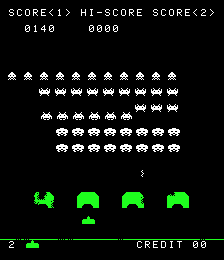
\includegraphics[width=9cm]{figures/space-invaders.png}
  \caption{A screenshot from the game \textit{Space Invaders}. The top line has reached the left side of the screen, so all enemy ships are in the midst of advancing forward \cite{spaceinvaders78}.}
  \label{fig:SpaceInvaders}
\end{figure}

In Space Invaders, enemies move in horizontal lines and occasionally shoot at the player, as shown in Figure \ref{fig:SpaceInvaders}. The player can move horizontally, to dodge projectiles and hide behind shields, and shoot back at the enemy. When a line of enemies hits a wall, the ships advance toward the player. As more enemy ships are destroyed, the lines become faster and faster, making them harder to hit. If a ship advances all the way to the player, the game ends and the player loses. Although the game becomes more difficult as the game progresses - ships become faster and shields become damaged - this difficulty has little to do with decisions made by the enemy ships; they just continue moving across the screen and shooting wildly.\\

\begin{figure}[H]
  \centering
  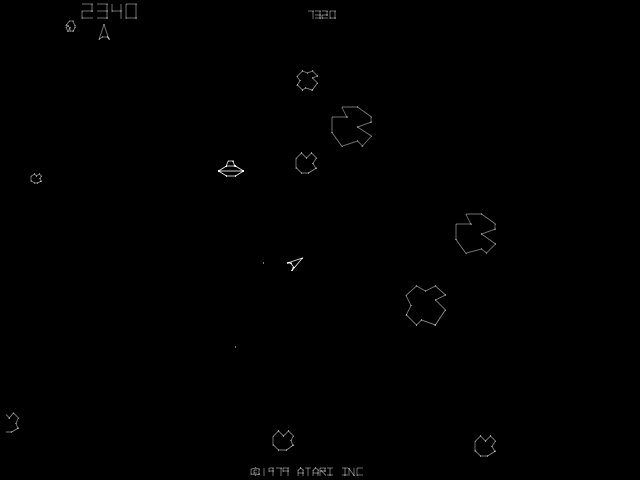
\includegraphics[width=9cm]{figures/Asteroids.png}
  \caption{A screenshot from the game \textit{Asteroids}. The player controls the triangular ship, and the flying saucer shoots in random directions. Another type of saucer exists in the game which fires directly at the player \cite{asteroids79}.}
  \label{fig:Asteroids}
\end{figure}

In Asteroids, the player's ship is freely movable in space. The ship must avoid or destroy asteroids and two different types of flying saucers. One saucer, the larger of the two, fires shots randomly. The other, smaller saucer targets the player directly and fires at them. In addition, the asteroids break into smaller asteroids as the player shoots them. Again, the difficulty of the game increases as asteroids break into smaller, faster pieces, but this does not reflect any choices made by the asteroids. The asteroids themselves simply move as inertia would dictate. Only the second saucer, which directly targets the player, has a semblance of intelligence. We infer from the nature of the gameplay that the saucer wants to destroy the player. By shooting right at the player, this enemy takes steps to achieve this goal. In contrast, the saucer which shoots randomly will sometimes try to achieve their goal (when the randomly-fired projectile moves in the general direction of the player) and sometimes will not (when the projectile moves in the complete opposite direction).\\

As time progressed, the intelligence of these enemies was improved with more intricate patterns (as in the space shooter Galaga (1981)) or in more heavily-scripted responses to inputs (as in the first-person shooter Half-Life (1998)) \cite{schw04}.
v
\begin{figure}[H]
  \centering
  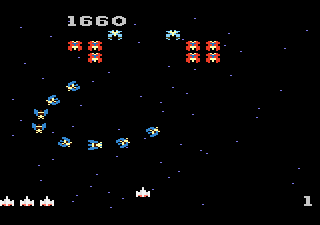
\includegraphics[width=8cm]{figures/ExampleGalaga.png}
  \caption{Four screenshots from the game \textit{Galaga}, showcasing (from 1 to 4) the movement of enemy ships \cite{galaga81}.}
  \label{fig:Galaga}
\end{figure}
Galaga, for example, uses curves and loops in the flight paths of enemy spaceships, as can be seen in Figure \ref{fig:Galaga}. Compared to the straight lines of \textit{Space Invaders}, the spaceships became more challenging to hit. Furthermore, the spaceships were programmed to fire when the player was directly below them, while \textit {Space Invaders} had enemies shooting seemingly at random \cite{schw04}.\\

In more recent titles, AI systems begin to show more intelligence. Some of this comes from more complex routines, as seen in the final boss of the game \textit{Final Fantasy IX}.

\lstset{caption={Section of AI script for Necron, an enemy in the game \textit{Final Fantasy IX} \protect\cite{ff9necron}.}, language=ff9code, label={lst:ff9Necron}}
\begin{lstlisting}
  set selectedattack = RandomAttack( attacklist )
  if ( selectedattack == Flare )
  set SV_Target = RandomInTeam( NotMatching(SV_PlayerTeam[STATUS_CURRENT], PETRIFY | DEATH | ZOMBIE | REFLECT) & NotMatching(SV_PlayerTeam[STATUS_AUTO], REFLECT) )
  elseif ( selectedattack == Holy )
  set SV_Target = RandomInTeam( NotMatching(SV_PlayerTeam[STATUS_CURRENT], PETRIFY | DEATH | ZOMBIE | REFLECT) & NotMatching(SV_PlayerTeam[STATUS_AUTO], REFLECT) )
  elseif ( selectedattack == Meteor )
  set SV_Target = SV_PlayerTeam
\end{lstlisting}

The boss, named Necron, has a variety of possible actions, three of which are shown in Listing \ref{lst:ff9Necron}. A random attack is selected from the list in line 1. For two of these attacks, a random character in the player's team is selected, provided that they do not have one of the listed special statuses, in lines 3 and 5. Two of these statuses (PETRIFY and DEATH) refer to when a character controlled by the player can no longer perform actions of their own \cite{ffIX00}. In this case, Necron targets a random character in the player's party who is not petrified or dead. The REFLECT status, on the other hand, prevents a player character from being affected by magic spells; the spells are reflected back at the opponent instead \cite{ffIX00}. For instance, if Necron did not exclude characters with the REFLECT status and tried to cast its Holy or Flare spell on a character with REFLECT, the spell would not damage said character. Instead, Holy or Flare would be reflected and deal damage to Necron, effectively causing the boss to damage itself. Thus, by excluding characters with REFLECT from the list of possible targets, Necron avoids making costly mistakes in battle. These checks improve the perceived ``intelligence'' of the boss; the AI does not waste actions attacking incapacitated players or causing itself harm from reflected magic.\\

While the \textit{Final Fantasy IX} example employs predetermined choices (apart from some random selection), other forms of intelligence come from more open-ended coding. For example, stealth games feature guards who must react to a variety of situations. One technique for such AI is to use fuzzy logic \cite{schw04}. Fuzzy logic deals with sets where membership is on a continuum \cite{zade65}. In this case, a guard in a stealth game would use this type of logic to transition from a calm state to a suspicious state to an alerted state as the player's presence is detected \cite{schw04}. Fuzzy logic is essential in this case to account for distance; if a player makes noise two rooms away, the guard shouldn't have as strong a reaction as when a player makes noise directly behind a guard. But, since a player may intentionally create distractions to exploit this suspicion, the AI for that guard cannot be too strongly scripted; what one player may do as a distraction another player may do accidentally, and the AI must account for these differences in play.\\

In many role-playing games (RPGs) like \textit{Final Fantasy IX}, the heroes live in fantastical worlds and often have the ability to heal themselves of their wounds with a quick potion or magic spell. While the player-controlled characters have these abilities, their AI-controlled opponents frequently do not. In rare cases where these enemies can heal themselves, this ability is often relegated to one-time uses determined by the game designers. For instance, an enemy may heal itself when it is close to death, but only the first time. This thesis concerns itself with designing an AI that can decide when it will use a healing ability, and is able to use game theory to analyze the resulting game.
% !TEX root = ../IS.tex
\chapter{Extensive Form Games}
\section{Basics of Game Theory}
Frequently used, and originally explored in economic contexts, game theory is the study of interactions between decision-makers. Antoine Cournot attempted to explain the decisions of duopolies (markets with only two sellers producing a product) in 1838 using the concept of strategic behavior \cite{webs14}. In this case, strategic behavior refers to scenarios where one person's decisions both affect and are affected by the decisions of other persons. Cournot later influenced Joseph Bertrand's 1883 work, which examined strategic decisions in product pricing. These early efforts were limited by standard economic methodologies; it wasn't until John von Neumann's 1928 proof of the minimax theorem and his later collaboration with economist Oskar Morgenstern that the modern field of game theory began \cite{webs14}. The strategies involved with game theory are used to explain collusion and subsequent breakdown of oligopolies like OPEC, and the symbiosis between sharks and pilot fish.\\

As we begin our study of game theory, it is important to precisely define what games are. A game is defined as an interaction constraining the actions a player can perform and the interests of players; Game theory involves the techniques used to analyze and determine solutions and outcomes of various games \cite{osbo94}. It is assumed that players in these games are both rational (they pursue well-defined objectives, generally in their own self-interest) and strategic (they take the knowledge and behavior of other decision-makers into account)\cite{osbo94}.\\

The goals of these players are represented using a utility function. In game theory, utility is the quantitative measure of a choice's value; this could be a monetary value or it could be expressed in terms of the happiness a player gains from that outcome, depending on the structure of the ``game''. A highly desired outcome for a player will have a higher utility than an undesirable outcome. Utility is the core of ``zero-sum games.'' In these games, one player's increase in utility corresponds to another player's equal loss in utility. For example, a player might earn \$5 in a zero-sum game by directly taking those \$5 from another player.

\section{Normal Form Games}
In the vast majority of human choices, a person will attempt to maximize their utility function; they will perform actions that benefit themselves. When there are two or more agents trying to maximize their utility, the interactions and choices between these agents, or players, become more and more complex. These interactions can be studied with game theory using the normal or strategic form.
\begin{define}
  A finite normal-form game is a tuple $(N, A, u)$ where:
  \begin{itemize}
  \item $N$ is a finite set of $n$ players, indexed by $i$
  \item $A=A_1\times\cdots\times A_n$, where $A_i$ is a finite set of actions available to player $i$. Each vector $a=(a_1,\cdots ,a_n)\in A$ is called an action profile.
    \item $u=(u_1,\cdots ,u_n)$ where $u_i : A \mapsto\mathbb{R}$ is a real-valued utility function for player $i$. \cite{shoh09}
\end{itemize}
\end{define}

In an arbitrary normal-form game, there are $n$ different players contained in the set $N$, where $n$ is a positive integer. For each of these players, there is also a finite set of actions that they can take. Player $N_i$ will have the action set $A_i$. The complete action set $A$ is determined by the Cartesian product of the action sets of each player. Within $A$, a vector $a$ is the action profile; an action profile, or outcome, represents the choice that each player makes \cite{osbo94}. The collection of mappings $u$ gives each action profile a particular value; these values determine which outcome is preferred by a player. In normal-form games, players are utility-maximizing agents; they will gravitate towards action profiles that give them higher utility.\\

An example of a normal-form game can be seen in the quintessential ``Prisoner's Dilemma'' example. This game is expressed in a 2x2 matrix, with one player's choices represented in the columns and the other player's choices represented in the rows of said matrix.

\begin{figure}[H]
  \centering
  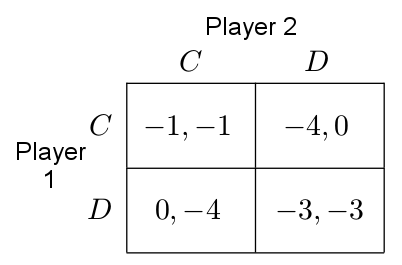
\includegraphics[width=7cm]{figures/ExampleGrid.png}
  \caption{The Prisoner's Dilemma, represented in a normal form matrix \cite{shoh09}.}
  \label{fig:prisoner}
\end{figure}

In Figure \ref{fig:prisoner}, the column labeled \textit{C} represents prisoner 2 cooperating with their partner, while the column labeled \textit{D} represents prisoner 2 defecting, telling the police that their partner is guilty. The rows \textit{C} and \textit{D} represent the same choices for prisoner 1. For this game, $A_i$ would be the set $\{C, D\}$, as those are the two choices that each prisoner can make. Thus, $A=A_1\times A_2 = \{(C, C), (C, D), (D, C), (D, D)\}$, or all four possible outcomes for this game. An action profile $a$ in this game would then be any of the ordered pairs in $A$; $(C,D)$, for instance, is an action profile. The ordered pairs of the matrix represent the values of each player's respective utility function in that outcome. In this case, their utility is the number of years in jail to which a player is sentenced. The mapping functions in $u$ correspond to the leniency of the courts; unfortunately, the quantitative functions in $u$ that the courts use in this example are unknown, and only the values at these specific points are known. When both prisoners cooperate, they both get one year in prison; their sentence is lighter without their confession. If only one prisoner confesses, that player gets off with not prison, while the other player gets four years in jail. If both prisoners rat out their partner for committing the crime, both prisoners get three years in prison.\\

From the perspective of an individual player, they must consider their options before proceeding. The best strategy of a player would be trivial if that player also knew which strategies the other player(s) were adopting \cite{shoh09}. This would be a \textit{pure strategy} option, where the player selects a single action and always that action. However, in the prisoner's dilemma, the two are being interrogated separately, and one player does not know the other player's choice. Thus, the prisoners must create a \textit{mixed strategy} by introducing probability to their decisions.

\begin{define}
  Let $(N,A,u)$ be a normal-form game, and for any set $X$ let $\Pi(X)$ be the set of all probability distributions over $X$. The set of mixed strategies for player $i$ is $S_i = \Pi(A_i)$, and the probability an action $a_i\in A_i$ will be played is denoted $s_i(a_i)$. A mixed-strategy profile is the Cartesian product of individual strategy sets $S_1\times\cdots\times S_n$ \cite{shoh09}.
\end{define}

For example of both pure and mixed strategies, consider a game where one player offers the other a choice of two different toys. The choosing player wants one of the toys, but not the other. Suppose that the identities of these toys are not hidden. In this case, the selecting player would use pure strategy and choose whichever toy gives them the most utility. Suppose instead that the toys are inside gift boxes. Since the choosing player does not know which box contains their desired toy, they have a 50-50 chance of picking the toy they want. Thus, they must use a mixed strategy. A pure strategy is a special case of mixed strategy, where the probability $s_i(a_i)$ is 1. With the mixed strategies determined, the players can find their best response to a mixed-strategy profile.

\begin{define}
  Let $S$ be the mixed-strategy profile for a normal-form game, and $s_{-i}$ be the set of strategy profiles disjoint from player $i$'s strategy profile $s_i$. Player $i$'s best response to $s_{-i}$ is a mixed strategy $s_i^*\in S_i$, such that $u_i(s_i^*,s_{-i}) \ge u_i(s_i, s_{-i})$ for all strategies $s_i\in S_i$ \cite{shoh09}.
\end{define}

For the toy choosing game, the mixed-strategy profile is the Cartesian product of player 1 and player 2's strategy sets. Player 1, the player offering the gifts, chooses to put the desired toy in box a or b. Player 2, the selecting player, chooses either box a or box b. The mixed-strategy profile would therefore be $(a, a), (a, b), (b, a), (b, b)$. Without knowing the strategy of other players, the most an agent can do is choose a strategy that is better than other strategies in all possible scenarios. This is known as the Nash equilibrium.

\begin{define}
  A strategy profile $s=(s_1,\dots ,s_n)$ is a Nash equilibrium if, for all agents i, $s_i$ is a best response to $s_{-i}$ \cite{shoh09}.
\end{define}

To find the Nash equilibrium for a player in this example, the action of the other player is assumed to be constant. For example, while determining player 1's Nash equilibrium, it is assumed that player 2 always confesses. This assumption limits player 1's decision to a single column in the normal form.
\begin{figure}[H]
  \centering
  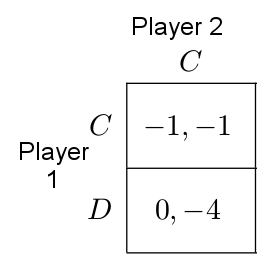
\includegraphics[width=5cm]{figures/ExamplePartialGrid1.png}
  \caption{Player 1's best response in the Prisoner's Dilemma, assuming Player 2 cooperates with Player 1}
  \label{fig:NashCol1}
\end{figure}

In Figure \ref{fig:NashCol1}, it is trivial to find the utility-maximizing strategy. In this case, the best response to player 2's cooperation is for player 1 to defect and accuse their partner: 1 year in prison or no time in prison. These steps are repeated for each of player 2's possible strategies.
\begin{figure}[H]
  \centering
  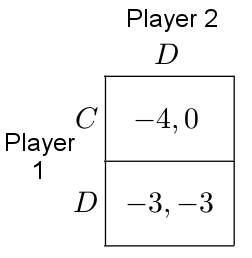
\includegraphics[width=5cm]{figures/ExamplePartialGrid2.png}
  \caption{Player 1's best response in the Prisoner's Dilemma, assuming Player 2 will defect against Player 1}
  \label{fig:NashCol2}
\end{figure}
So, assuming player 2 will defect to the police, player 1's best response is to defect as well: 3 years in prison or 4 years in prison. Since the best response is the same for all of player 2's strategies, this player will always choose this option. Using the same process for player 2 returns the same best response.

Thus, the Nash equilibrium is that both prisoners will defect, and both will get 3 years in prison. 

\begin{proof}
  Let $G=(N, A, u)$ be a normal-form game. $N = \{n_1, n_2\}$ is the set of players in the game. $A=A_1\times A_2$ is the set of actions in the game, where $A_1=\{c_1, d_1\}$ is the set of actions available to player 1, and $A_2=\{c_2, d_2\}$ is the set of actions available to player 2. Therefore, $A=\{(c_1, c_2), (c_1, d_2), (d_1, c_2), (d_1, d_2)\}$. The utility function $u=(u_1, u_2)$. $u_1=(c_1, c_2)\mapsto -1, (c_1, d_2)\mapsto -4, (d_1, c_2)\mapsto 0, (d_1, d_2)\mapsto -3$, and $u_2=(c_1, c_2)\mapsto -1, (c_1, d_2)\mapsto 0, (d_1, c_2)\mapsto -4, (d_1, d_2)\mapsto -3$.\\

  Let $s^*_1$ be a mixed strategy for $n_1$ where $n_1$ chooses action $d_1$. Since there are only two other players, the set of strategy profiles disjoint from $s_1$ is the same as $s_2$, the set of strategy profiles for $n_2$. Thus, $n_1$ has $s^*_1$ as a best response to $s_2$ if $u_1(s^*_1, s_2)\ge u_1(s_i, s_2)$ for all possible actions $s_i\in A_1$ and all strategies in $s_2$.\\
  
  $u_1(d_1, c_2)\ge u_1(c_1, c_2) \Rightarrow 0\ge -1$\\
  
  $u_1(d_1, c_2)\ge u_1(d_1, c_2) \Rightarrow 0\ge 0$\\

  $u_1(d_1, d_2)\ge u_1(c_1, d_2) \Rightarrow -3\ge -4$\\

  $u_1(d_1, d_2)\ge u_1(d_1, d_2) \Rightarrow -3\ge -3$\\

  $s^*_1$ is greater than or equal to all possible actions in $A_1$ and for all strategies in $s_2$. Thus, $s^*_1=d_1$ is the best response for player $n_1$.\\

  Let $s^*_2$ be a mixed strategy for $n_2$ where $n_2$ chooses action $d_2$. Since there are only two other players, the set of strategy profiles disjoint from $s_2$ is the same as $s_1$, the set of strategy profiles for $n_1$. Thus, $n_2$ has $s^*_2$ as a best response to $s_1$ if $u_2(s^*_2, s_1)\ge u_2(s_i, s_1)$ for all possible actions $s_i\in A_2$ and all strategies in $s_1$.\\
  
  $u_1(c_1, d_2)\ge u_1(c_1, c_2) \Rightarrow 0\ge -1$\\

  $u_1(c_1, d_2)\ge u_1(c_1, d_2) \Rightarrow 0\ge 0$\\

  $u_1(d_1, d_2)\ge u_1(d_1, c_2) \Rightarrow -3\ge -4$\\

  $u_1(d_1, d_2)\ge u_1(d_1, d_2) \Rightarrow -3\ge -3$\\

  $s^*_2$ is greater than or equal to all possible actions in $A_2$ and for all strategies in $s_1$. Thus, $s^*_2=d_2$ is the best response for player $n_1$. A strategy set $(s_1,\dots ,s_n)$ is a Nash equilibrium if $s_i$ is the best response for all players $i$. Therefore, the strategy profile $(d_1, d_2)$ is a Nash equilibrium for game $G$.
\end{proof}

Not all games have a Nash equilibrium; take the normal-form representation of rock-paper-scissors, for instance. Assume that the utility function award players 1 point for winning the game, -1 point for losing the game, and 0 points for a draw. We will position Player 1 be on the left side of the matrix, and Player 2 be on the top of the matrix.
\begin{figure}[H]
  \centering
  \begin{tabular}{r r | c | c | c |}
    &\multicolumn{1}{c}{}&\multicolumn{1}{c}{}&\multicolumn{1}{c}{Player 2}&\multicolumn{1}{c}{}\\
    Rock-Paper-Scissors &\multicolumn{1}{c}{}&\multicolumn{1}{c}{Rock}&\multicolumn{1}{c}{Paper}&\multicolumn{1}{c}{Scissors} \\ \cline{3-5}
    & Rock & (0, 0) & (-1, 1) & (1, -1) \\ \cline{3-5}
    Player 1 & Paper & (1, -1) & (0, 0) & (-1, 1) \\ \cline{3-5}
    & Scissors & (-1, 1) & (1, -1) & (0, 0) \\ \cline{3-5}
  \end{tabular}
  \caption{The normal-form representation of the game Rock-Paper-Scissors}
  \label{fig:RPS}
\end{figure}

Every row and every column in this Figure \ref{fig:RPS} has the same three results, and none of the choices is a winning strategy for more than one situation. Rock may beat Scissors, but it loses to Paper. If the Nash equilibrium of Player 1 is investigated, each possible action by Player 2 results in a different best response for Player 1. Thus, there can be no equilibrium.

\subsection{Non-Simultaneous Games}

It is important to recognize in these two examples that both players are making their choice simultaneously. Games without simultaneous actions are not so easily expressed in normal form. For example, take a game of tic-tac-toe. For simplicity, assume that the game is played with a 2x2 board instead of a 3x3 board. Assume the utility function award players 1 point for winning the game, -1 point for losing the game, and 0 points for a draw. Let UL be a piece in the upper left square, UR the upper right square, LL the lower left square, and LR the lower right square. We position Player 1 be on the left side of the matrix, and Player 2 be on the top of the matrix. Assume Player 1 has the first turn.\\
\begin{figure}[H]
  \centering
  \begin{tabular}{r r | c | c | c | c |}
    &\multicolumn{1}{c}{}&\multicolumn{1}{c}{}&\multicolumn{1}{c}{Player 2}&\multicolumn{1}{c}{}\\
    \multicolumn{1}{c}{2x2 tic-tac-toe}&\multicolumn{1}{c}{}&\multicolumn{1}{c}{UL}&
    \multicolumn{1}{c}{UR}&\multicolumn{1}{c}{LL}&\multicolumn{1}{c}{LR}\\ \cline{3-6}
    & UL & x & (0, 0) & (0, 0) & (0, 0) \\ \cline{3-6}
    Player 1 & UR & (0, 0) & x & (0, 0) & (0, 0) \\ \cline{3-6}
    & LL & (0, 0) & (0, 0) & x & (0, 0) \\ \cline{3-6}
    & LR & (0, 0) & (0, 0) & (0, 0) & x \\ \cline{3-6}
  \end{tabular}
  \caption{The first two moves of a tic-tac-toe variant using a 2x2 game board.}
  \label{fig:2x2TTT}
\end{figure}

Figure \ref{fig:2x2TTT} shows the normal form for the first two moves of this game. Since each player has only placed a single piece, neither one has won yet; thus, the utility for each space is (0,0). There are four spaces in the matrix marked with an 'x'. These spaces are infeasible; it is against the rules for someone to play on the same square as someone else. Both players have made their first move, and it is Player 1's turn once again.\\
\begin{figure}[H]
  \centering
  \begin{tabular}{r r | c | c | c | c |}
    &\multicolumn{1}{c}{}&\multicolumn{1}{c}{}&\multicolumn{1}{c}{Player 2}&\multicolumn{1}{c}{}\\
    \multicolumn{1}{c}{2x2 tic-tac-toe}&\multicolumn{1}{c}{}&\multicolumn{1}{c}{UL}&
    \multicolumn{1}{c}{UR}&\multicolumn{1}{c}{LL}&\multicolumn{1}{c}{LR}\\ \cline{3-6}
    & (UL, UR) & x & x & (1, -1) & (1, -1) \\ \cline{3-6}
    & (UL, LL) & x & (1, -1) & x & (1, -1) \\ \cline{3-6}
    & (UL, LR) & x & (1, -1) & (1, -1) & x \\ \cline{3-6}
    & (UR, UL) & x & x & (1, -1) & (1, -1) \\ \cline{3-6}
    & (UR, LL) & (1, -1) & x & x & (1, -1) \\ \cline{3-6}
    Player 1 & (UR, LR) & (1, -1) & x & (1, -1) & x \\ \cline{3-6}
    & (LL, UL) & x & (1, -1) & x & (1, -1) \\ \cline{3-6}
    & (LL, UR) & (1, -1) & x & x & (1, -1) \\ \cline{3-6}
    & (LL, LR) & (1, -1) & (1, -1) & x & x \\ \cline{3-6}
    & (LR, UL) & x & (1, -1) & (1, -1) & x \\ \cline{3-6}
    & (LR, UR) & (1, -1) & x & (1, -1) & x \\ \cline{3-6}
    & (LR, LL) & (1, -1) & (1, -1) & x & x \\ \cline{3-6}
  \end{tabular}
  \caption{The full normal form representation of a 2x2 tic-tac-toe variant}
  \label{fig:full2x2TTT}
\end{figure}

Since the game board was shrunk for this example, the game ends with Player 1 always winning on their second turn. But even in this simplified game, the normal form in Figure \ref{fig:full2x2TTT} quickly becomes convoluted and cluttered. While the infeasible actions are fairly self-evident in Figure \ref{fig:2x2TTT}, illegal moves are less obvious in Figure \ref{fig:full2x2TTT}.
\begin{figure}[H]
  \centering
  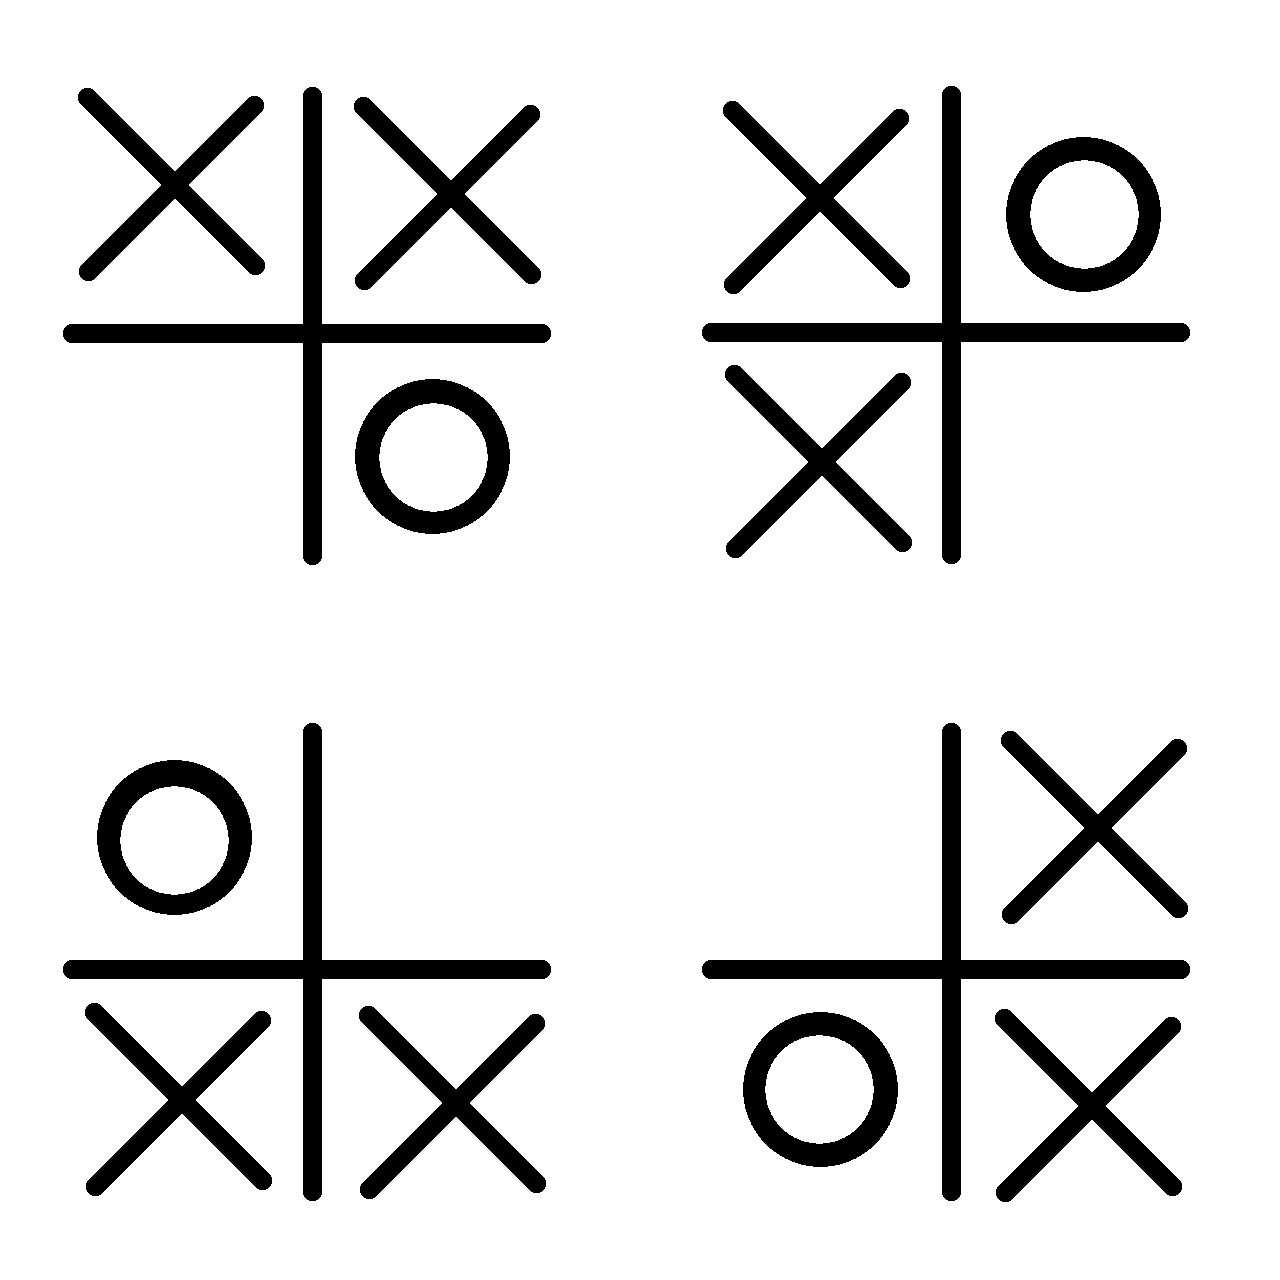
\includegraphics[width=6cm]{figures/TTTRotation.png}
  \caption{Rotational symmetry in a 2x2 tic-tac-toe game}
  \label{fig:2x2TTTRotation}
\end{figure}
There are also repeated game configurations: the outcome \{(UL, UR), (LR)\} is rotationally symmetrical to \{(LL, UL), (UR)\}, \{(LR, LL), (UL)\}, and \{(UR, LR), (LL)\}, as is evident in Figure \ref{fig:2x2TTTRotation}. Furthermore, the game \{(UL, UR), (LR)\} is identical to \{(UR, UL), (LR)\}. With so many extraneous spaces in the normal-form representation, it is no longer sufficient to represent player choices for games with sequential actions. Instead, these games are better represented in extensive-form trees.\\

\section{Extensive Form Trees}
In a turn-based, or extensive-form game, players do not make simultaneous actions. This leads to larger variety in gameplay. A simultaneous game like Rock-Paper-Scissors relies on chance; tic-tac-toe relies on players anticipating the future choices their opponents will make. There are two types of extensive-form games: perfect-information and imperfect-information. In perfect-information games, all players know which turn of the game they are at, while imperfect-information games have turns that are indistinguishable from others based on information available to the player. We will be dealing with perfect-information games.\\

\begin{define}
  A finite perfect information game in extensive form is a tuple $G = (N, A, H, Z, \chi, \rho, \sigma, u)$ where:
  \begin{itemize}
  \item $N$ is a set of n players;
  \item $A$ is a single set of actions;
  \item $H$ is a set of non-terminal, choice nodes;
  \item $Z$ is a set of terminal nodes, disjoint from $H$;
  \item $\chi: H\mapsto 2^A$ is the action function, mapping a set of possible actions to each choice node;
  \item $\rho: H\mapsto N$ is the player function, mapping to each non-terminal node a player who makes an action at said node;
  \item $\sigma: H\times A\mapsto H\bigcup Z$ is the successor function, mapping a choice node and an action to a new choice or terminal node. $\forall h_1, h_2\in H$ and $a_1, a_2\in A$, if $\sigma(h_1, a_1)=\sigma(h_2, a_2)$, then $h_1=h_2$ and $a_1=a_2$;
  \item $u=(u_1,...,u_n)$, where $u_i:Z\mapsto \mathbb{R}$ is a real-valued utility function for each player $i$ on a terminal node $Z$ \cite{shoh09}.
  \end{itemize}
\end{define}

As in the normal-form definition, there are $n$ players in the game, contained in the set $N$. $A$ is the set of all actions that could be performed in the course of the game. The set $H$ contains any and all choices or turns that do not end the game, while $Z$ contains all choices or turns that do end the game. The mapping function $\chi$ allocates the choices in $H$ a subset of possible actions from the set $A$, and the mapping function $\rho$ assigns these choices to the players who make them. $\sigma$ takes the actions assigned with $\chi$ and uses them to connect various nodes in $H$ and $Z$ together, creating the sequence of events in the game. Finally, $u$ contains utility functions for each player that determines their individual utility at each of the terminal nodes in $Z$.\\

\begin{figure}[H]
  \centering
  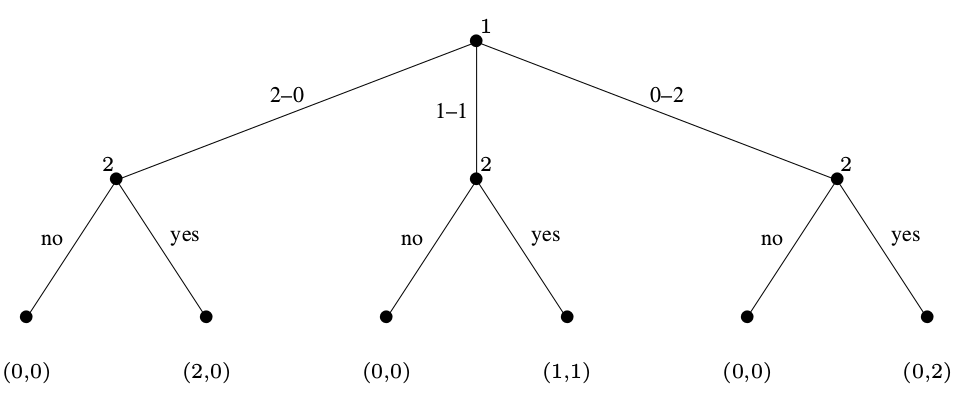
\includegraphics[width=10cm]{figures/ExampleTree.png}
  \caption{An extensive-form tree for The Sharing Game \cite{shoh09}}
  \label{fig:sharingTree}
\end{figure}

An example of the extensive-form tree can be seen in Figure \ref{fig:sharingTree}. The six leaf nodes of this tree are the elements of the set $Z$, while the other nodes are contained in $H$. The $H$ nodes are labeled either 1 or 2, denoting from the $\rho$ function which player is making the choice at that node. The $Z$ nodes each have a pair, denoting the utility each player will gain if the game ends in that particular way. The actions $A$ are denoted in the lines connecting the nodes together. In this game, the three actions from the root node are the methods of sharing 2 presents between 2 people. The second player, once the first player has distributed the presents in a particular way, chooses whether to accept the distribution or not.\\

To explore this definition, return to the game of tic-tac-toe. Let $N={N_1, N_2}$ be the set of players in the game. In this game, $A$ is the set of playing on one of the open spaces on the board; for the first move of the game, $A$ is the set of 9 open spaces on the board, for the second move, $A$ is the set of the remaining 8 spaces. For a game of tic-tac-toe, $H$ contains configuration of the board where neither player has three in a row and there are still open squares on the board. $Z$, on the other hand, contains the board configurations where one player has three in a row or all spaces have been claimed. For tic-tac-toe, the $\chi$ function removes illegal actions from a node, which in tic-tac-toe would be playing on an occupied square. Thus, the $\chi$ function leaves the choice nodes at each successive turn with fewer and fewer available actions. Since there are only two players, the $\rho$ function alternates between players after each action.

\begin{figure}[H]
  \centering
  
\includegraphics[width=16cm]{figures/TTTExtTree.png}
  \caption{The extensive-form representation of a 2x2 tic-tac-toe game}
  \label{fig:2x2TTTExtForm}
\end{figure}

Figure \ref{fig:2x2TTTExtForm} shows the extensive-form version of the 2x2 tic-tac-toe variant in Figure \ref{fig:full2x2TTT}. In comparison to the normal-form representation, the extensive-form tree can convey the sequence and flow of the game more clearly. Since the $\chi$ function of an extensive-form game only maps possible actions, the tree does not have the same infeasible nodes as the normal-form representation. This tree has the same issues of rotational symmetry as in the normal form, but in this particular example, the four subtrees connected to the root are all rotationally symmetrical to each other.

\subsection{Equilibria in Extensive-Form}
Nash equilibria can be found in extensive-form games as well, and are defined the same as in normal-form games. However, a pure strategy in an extensive-form game requires the player's strategy to contain the decision at every choice node, even if that node is unreachable by other choices in said strategy.\\
\begin{define}
  Let $G = (N, A, H, Z, \chi, \rho, \sigma, u)$ be a perfect-information extensive-form game. The pure strategies of player $i$ consist of the Cartesian product $\Pi_{h\in H, \rho(h)=i}\chi(h)$ \cite{shoh09}.
\end{define}
Given a perfect-information game, a player's pure strategy is the set of choices mapped by $\chi$ from each of that player's choice nodes $h$. It is a complete specification of the choices that a player determines they should make \cite{shoh09}. Since the actions of all other players are known in an extensive-form game, it is not necessary to introduce probabilities to determine a Nash equilibrium. Instead, Nash equilibria can be found using backwards induction.
%\begin{algorithm}
%  \caption{Backwards Induction \cite{shoh09}}
%  \begin{algorithmic}[1]
%    \Procedure {BackwardInduction}{node $h$}
%    \If{$h\in Z$}
%    \State Return $u(h)$
%    \Comment If $h$ is a leaf node, return the utility of that outcome
%    \EndIf
%    \For{$a\in\chi(h)$}
%    \State $util\_at\_child \gets BackwardInduction(\sigma(h, a))$
%    \Comment Recursively check each child of $h$
%    \If{$util\_at\_child_{\rho(h)}>best\_util_{\rho(h)}$}
%    \State $best\_util\gets util\_at\_child$\\
%    \Comment $best\_util$ holds the utility which is maximized for the player $\rho(h)$
%    \EndIf
%    \EndFor
%    \State Return $best\_util$
%    \EndProcedure
%  \end{algorithmic}
%\end{algorithm}

\lstset{language=pseudocode, label={lst:BackwInd}, caption={The Backward Induction algorithm for extensive-form game trees \cite{shoh09}.}}
\begin{lstlisting}[language=pseudocode]
  Procedure BackwardInduction(node h)
  if(h in Z)
      return u(h)
      //If h is a leaf node, return the utility of that outcome
  end if
  for(a in %*$\chi$*(h))
      util_at_child = BackwardInduction(%*$\sigma(h, a)$*)
      //Recursively check each child of h
      if(util_at_child%*$_{\rho(h)}$* > best_util%*$_{\rho(h)}$*)
          best_util = util_at_child
          //best_util holds the node which maximizes the utility of player %*$\rho$*(h)
      end if
  end for
  return best_util
  end Procedure
\end{lstlisting}

Backwards induction determines a dominant strategy for a particular game. The algorithm's base case is at line 2, where $h$ is in the set of terminal nodes in $Z$, or the leaves of the extensive-form tree. At these leaves the game is over, and the utility of that outcome is returned by the algorithm. When the node in question is not a terminal node, the algorithm checks the utility of each of that node's children at line 5. Since the child nodes may have their own children, line 6 recursively checks each child and gets the utility of that node. In lines 7 and 8, the backwards induction algorithm determines which node provides the player at node $h$ (as determined by the mapping function $\rho$) the maximum amount of utility. This node is returned in line 12.\\

\begin{figure}[H]
  \centering
  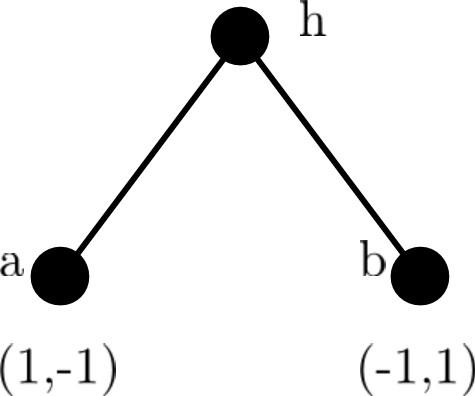
\includegraphics[width=4cm]{figures/ExampleBackwardInduction.png}
  \caption{A small extensive-form tree. The outcome is dependant on the player mapped by $\rho(h)$.}
  \label{fig:BackwardInduction}
\end{figure}
For example, examine the extensive-form tree for a two-player game in Figure \ref{fig:BackwardInduction}. with a root and two child, terminal nodes. At the leaf node $a$, player 1 has positive utility while player 2 has negative utility; at leaf node $b$, player 2 has positive utility and player 1 has negative utility. Since both players are utility-maximizing agents, the choice of the outcome is determined by whichever player happens to be making the decision, as mapped by $\rho(h)$. Suppose that Figure \ref{fig:BackwardInduction} is a subtree in a larger game. Further suppose that, in this larger game, the subtree in Figure \ref{fig:BackwardInduction} always has player 1 making the choice at node $h$. Given this scenario, player 1 will always perform the action that gets them to node $a$. Thus, node $h$ can be replaced by $a$, with $b$ being removed from the tree entirely, and the rest of the game will be unchanged. If the entire tree for a game is mapped out, then this process can be repeated all the way up to a root node; at that point, .
% !TEX root = ../IS.tex
\chapter{Machine Learning}
\section{Decision Trees}
The goal of a machine learning problem is, of course, to learn; given a task with a particular performance measure, the performance can be improved through some kind of training or experience. Often, this involves evaluating a general case for the task from a set of specific examples \cite{mitc97}. One of the more common machine learning techniques is the decision tree. It can approximate discrete-valued functions \cite{mitc97} and automatically classify data \cite{sega07}. Generally, decision trees focus on problems with attribute-value pairs; an attribute \textit{Temperature} may have the possible values \textit{Hot, Cold, Warm, Cool} \cite{mitc97}.\\

When creating a decision tree, one must begin with example data to analyze. This may be historical data, looking at the same problem from previous years, or a set of example problems. In order to form an effective tree, these data are split into two groups: a training set, and a testing set. The training set is used to create the tree, while the testing set is used to find the approximate error of the tree. It is important that these two sets are disjoint; the error of a tree cannot be accurately determined if it isn't analyzing new data in the testing phase.

\subsection{ID3 Algorithm}
The ID3 algorithm for decision trees, like most decision tree algorithms, uses a top-down greedy search \cite{mitc97}. The algorithm begins by evaluating the input data by individual attributes in the training set. For each attribute, the algorithm attempts to classify the entire data set using only that attribute. Whichever attribute was the most successful on its own becomes the root of the tree. Then, for each possible value of that root attribute, a descendant node is created and the training set is split accordingly. Then, for each descendant node and its respective subset of training data, the process is repeated.\\

To find the best attribute at each node of the tree, the ID3 algorithm uses the statistical property information gain. Information gain utilizes entropy, or the relative impurity of a data collection.
\begin{define}
  For a set of training data $S$ with $n$ different target values, Entropy(S)$\equiv\sum_{i=1}^n-p_i$log$_2p_i$, where $p_i$ is the proportion of S with a target value of $i$.
\end{define}
Entropy calculations define 0log(0) as 0. The logarithm can have any base value, but two is often used; a base of 2 conveys the expected encoding length in bits \cite{mitc97}. Assuming the base value is 2, an entropy value of 0 occurs when all data set elements have the same target value $i$, and a  set with a 50/50 split between two target values will have an entropy value of 1. Ideally, a decision tree classifies data into sets with low entropy, as this indicates an accurate tree structure.\\

In order to minimize entropy in the classified data, the information gain of each attribute is calculated. Information gain is defined as the expected reduction in entropy caused by splitting the training data by a particular attribute.
\begin{define}
  For an attribute $A$ and a set of training data $S$, the Information Gain(S, A)$\equiv$ Entropy(S) $-\sum_{v\in Values(A)}\frac{||S_v||}{||S||}$ Entropy$(S_v)$, where $Values(A)$ is the set of possible values for the attribute $A$, and $S_v$ is the subset of $S$ where $A$ has value $v$.
\end{define}
Each attribute $A$ for a given node is tested, with each of its possible values used in the summation. For these values, the entropy of each subset $S_v$ is calculated, then scaled by the size of $S_v$ compared to $S$.\\

\begin{figure}[H]
  \centering
  \begin{tabular}{| c | c | c |}
    Month & Tickets & Weekend \\ \hline
    3 & 25 & 0 \\ \hline
    8 & 45 & 1 \\ \hline
    8 & 25 & 0 \\ \hline
  \end{tabular}
  \caption{A sample data set with three attributes and three entries}
  \label{fig:ExampleEntropy}
\end{figure}

For example, consider the data set in Figure \ref{fig:ExampleEntropy}. The \textit{Month} attribute is the numeric value of the calendar month, \textit{Tickets} is the number of tickets sold to an event, and \textit{Weekend} is a Boolean value whether the event is on a weekend or not. Suppose that the target attribute of this set is \textit{Weekend}. The \textit{Weekend} attribute has two values represented in the set: 0 and 1. Of the data points in Figure \ref{fig:ExampleEntropy}, only one took place on a weekend. Thus, the $p_i$ for Weekend=True is $\frac{1}{3}$, which we round to $.33$. The $p_i$ for Weekend=False is therefore $\frac{2}{3}$ rounded to $.66$. Recall that the entropy formula is Entropy(S)$\equiv\sum_{i=1}^n-p_i$log$_2p_i$. Let $i=1$ be the attribute Weekend=True and $i=2$ be the attribute Weekend=False. The entropy for the target attribute \textit{Weekend} is therefore the sum $-.66$log$_2(0.66) + -.33$log$_2(.33)$, or approximately 0.9235. For this specific set, all attributes have two possible values, and will thus have a $\frac{1}{3}$ and $\frac{2}{3}$ split. In this example, the entropy will be the same for any target attribute.\\

To reduce this entropy, the ID3 algorithm finds the information gain for the two non-target attributes: \textit{Month} and \textit{Tickets}. Beginning with \textit{Month}, the information gain is $0.9235 - \frac{1}{3}$(Entropy(v=3)) $+ \frac{2}{3}$(Entropy(v=8)). At \textit{Month} 3, the entropy of the set is 0, as it contains a single element. The entropy of the subset at \textit{Month}=8 is 1, as the set has a 50/50 split along the target \textit{Weekend} attribute. Thus, the information gain for \textit{Month} is $0.9235 - \frac{2}{3}$, or 0.2568. Separating the data set along the \textit{Month} attribute does help in classifying the events by weekend, but the August events are now split 50/50.\\

The \textit{Tickets} attribute has an information gain of $0.9235 - \frac{2}{3}$(Entropy(v=25)) $+ \frac{1}{3}$(Entropy(v=45)). Since all elements in the subset of $S$ where \textit{Tickets}=25 have a target values of 0, the entropy is 0. The same is true of the subset where \textit{Tickets}=45. Thus, the information gain from this attribute is 0.9235. This does not indicate that no information was gained, this indicates that all entropy was removed from the set. All subsets are homogeneous when separating subsets by \textit{Tickets}.

Once the maximum information gain for a set has been determined, the ID3 algorithm uses the resulting subsets and recursively creates new subtrees for the subsets. This process continues until the entropy for the entire tree is 0. Once a tree has been created with the algorithm, it is simple to classify new data. Starting at the root of the tree, each target attribute is tested recursively, moving from one node to another down the tree \cite{sega07}.\\

\lstset{language=pseudocode, label=lst:ID3, caption={The ID3 Decision Tree algorithm \cite{mitc97}.}}
\begin{lstlisting}
Procedure ID3(TrainingSet S, TargetAttribute t, AttributeSet A)
create node Root
TestEntropy = True, TestAttributeValue = S[0]
for(i in S)  //Check whether the TrainingSet is uniform on t
  if(TargetAttribute[i]!=TestAttributeValue) TestEntropy=False
  //One of the elements has a different value for t
  end if
end for
if(TestEntropy is True) return root with label value of t
//This is a single-node tree; all elements in S have the same t value
else if(A is EmptySet) return Root with mode(t)
//There are no more attributes to check, return most common t value
else
//Determine optimal split for S
  OptimalInformationGain = 0
  for(attr in A)
    InformationGain = Entropy(S)
    EntropySum = 0
    for(val in attr)
      S_v = {S:Value(attribute)=val} //S_v contains the elements of S which have val for attr
      EntropySum = EntropySum + size(S_v)/size(S) * Entropy(S_v)  //Add entropy for each possible val for attr
    end for
    InformationGain = InformationGain - EntropySum
    //This is the information gain from splitting S on attr
    if(InformationGain > OptimalInformationGain)
      OptimalInformationGain = InformationGain
      //The maximum InformationGain value is stored
    end if
  end for
  //The optimal information gain has been found on attr
  Root.Label = attr
  for(val in attr)
    create Branch(val_i)
    NewTrainingData = {s in S:Value(attr)=val_i}
    if(NewTrainingData is EmptySet)
      create Leaf with mode(t) on S
    else
      add ID3(NewTrainingData, t, A-attr) as subtree
    end if
  end for
end if
return Root
end Procedure
\end{lstlisting}

In line 2 of the algorithm in Listing \ref{lst:ID3}, the root of the tree (or subtree) is created. The first base case to test is whether or not the TargetAttribute $t$ has the same value for every element in the TrainingSet $S$. This base case refers to a set $S$ with an entropy of 0, that requires no further classification, and begins at line 5. The second base case, starting on line 15, occurs when no non-target attributes remain in $A$. Without attributes, there is no way to further classify $S$, and the most common value for $t$ is used as the label for this node. This leaves the recursive case. The first step is to find the optimal information gain, and thus the next attribute used to split $S$. The loop at line 21 checks each attribute in $A$ for the largest reduction in entropy, and the attribute that created this reduction is saved as the label for the Root node on line 38. Line 39's loop prepares the data to be analyzed by the next levels of the decision tree. First, a new branch is created linking Root and the to-be-created subtree, with each branch labeled with a possible value of the attribute used in the split. Training data is split along this same value. If one of the new training data splits has no elements, a leaf node is labeled with the most common value of $t$ in $S$. This step is done to accommodate future data sets; while the training set may not have had any examples with that attribute value, other sets might and thus the tree assumes the most common value is correct. All other splits of $S$ are recursively passed to ID3() in line 45, along with $t$ and the AttributeSet $A$ (sans the attribute just used).\\

Suppose someone wanted to use the data set in Figure \ref{fig:ExampleEntropy} to predict ticket sales. We have the TargetAttribute \textit{Tickets}, an AttributeSet \{\textit{Month, Weekend}\}, and a TrainingSet = \{(3, 25, 0), (8, 45, 1), (8, 25, 0)\}. After creating a root node, we first check if all values of the TargetAttribute \textit{Tickets} are the same in the data set. This is not the case (two instances of 25 tickets sold, one instance of 45 tickets sold), so we continue through the algorithm. The second step is to check if AttributeSet is the empty set; this also is not the case. Thus, we enter the meat of the algorithm. We choose an attribute from AttributeSet and find the information gain of that attribute. Recall that the information gain of an attribute $A$ and set of examples $S$ is equal to Entropy$(S)-\sum_{v\in Values(A)}\frac{||S_v||}{||S||}$ Entropy$(S_v)$. As established previously, the entropy of our TrainingSet is approximately $0.9235$. With three entries, $||S||=3$. To start, let $A$ be the attribute \textit{Month}, which has possible values 3 and 8. For $v=3$, the subset $S_v$ has one entry, so $||S_v||=1$. In a set with only one entry, the entropy will necessarily be 0. For $v=8$, $S_v$ has two entries and $||S_v||=2$. The two August entries have different values for \textit{Tickets}, so the proportion $p_i$ will be $\frac{1}{2}$. Thus, the entropy of $S_v$ for $v=8$ will be $-.5 $log$_2(.5)$, which is $.5$. Thus, the information gain for attribute \textit{Month} is:
\begin{align*}
  .9235 - [(\frac{1}{3}*0) + (\frac{2}{3}*.5]\\
  .9235 - [0 + \frac{1}{3}]\\
  .5902
\end{align*}

Next, we repeat this formula for attribute \textit{Weekend}. This attribute also has two possible values, 1 and 0. For $v=1$, there is only one entry; $||S_v||$ will again be 1 and entropy will again be zero. For $v=0$, there are two entries, so $||S_v||=2$. Both of these entries have the same value for the target attribute \textit{Tickets}, so the entropy on $S_v$ for $v=0$ is also 0. Thus, the information gain for attribute \textit{Weekend} is:
\begin{align*}
  .9235 - [(\frac{1}{3}*0) + (\frac{2}{3}*0)]\\
  .9235 - [0 + 0]\\
  .9235
\end{align*}
We find that the \textit{Weekend} attribute has a higher information gain than the \textit{Month} attribute. So, the next step in the algorithm is to label the root node with \textit{Weekend}. 

\begin{figure}[H]
  \centering
  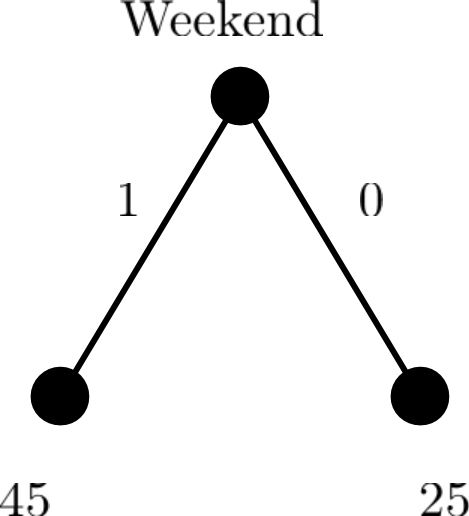
\includegraphics[width=4cm]{figures/ID3Example.png}
  \caption{A decision tree made with the ID3 algorithm, based on the training set in Figure \ref{fig:ExampleEntropy} with TargetAttribute \textit{Tickets}}
  \label{fig:ID3Example}
\end{figure}
Then, for the two possible values of \textit{Weekend}, the algorithm creates a new branch for that value. For the branch where $v=1$, the ID3 algorithm is called with TargetAttribute \textit{Tickets}, AttributeSet \{\textit{Month}\}, and TrainingSet = \{(8, 45, 1)\}. In this recursive call, the TargetAttribute \textit{Tickets} is uniform. Thus, the recursive call returns a node labeled with the value of \textit{Tickets}, 45. For the branch where $v=0$, the ID3 algorithm is called with TargetAttribute \textit{Tickets}, AttributeSet \{\textit{Month}\}, and TrainingSet = \{(3, 25, 0), (8, 25, 0)\}. Again, the TargetAttribute \textit{Tickets} is uniform, so a node labeled with the value of \textit{Tickets}, 25, is returned. Thus, the ID3 algorithm returns the tree in Figure \ref{fig:ID3Example}.\\

\subsection{Special Cases}
While the data in Figure\ref{fig:ExampleEntropy} use numeric data, the small sample set allows the ID3 algorithm to treat them as discrete values. However, decision trees must also be able to classify along continuous-valued attributes.
\begin{figure}[H]
  \centering
  \begin{tabular}{| c | c |}
    Temperature & PlayTennis \\ \hline
    40 & No \\ \hline
    48 & No \\ \hline
    60 & Yes \\ \hline
    72 & Yes \\ \hline
    80 & Yes \\ \hline
    90 & No \\ \hline
  \end{tabular}
  \caption{A sample data set containing the temperature in degrees Fahrenheit and whether or not tennis was played \cite{mitc97}.}
  \label{fig:rangedValue}
\end{figure}

\begin{exmp}
  Take for example the data set in Figure \ref{fig:rangedValue}. This data set is being analyzed to determine which temperatures are ideal for playing tennis. For six days, the temperature in degrees Fahrenheit and whether people played tennis was recorded.\\
\end{exmp}

Since only six temperatures were recorded, this training set cannot use these findings as discrete values. If it was classified discretely, then any temperature not explicitly in the training set (68 degrees, for instance) would not be accurately classified. Thus, the temperature must be treated as a continuous-valued attribute.\\

To deal with a continuous-valued attribute $A$, a new Boolean attribute $A_c$ is created where $A_c$ is true if $A<c$ and false otherwise \cite{mitc97}. For the dataset in Figure \ref{fig:rangedValue}, $c$ should be set to a value where the target attribute (in this example, whether people played tennis) changes. Thus, for this example, the thresholds between whether people do play tennis or when they dont happen between 48 and 60 degrees, and between 80 and 90 degrees. The simplest method is to take the average of the two temperatures, so $A_{c1}=\frac{48+60}{2}=54$ and $A_{c2}=\frac{80+90}{2}=85$. Therefore, based on the training data, a decision tree classifying tennis by outdoor temperature would predict ``No'' when temperature is below 54 degrees or above 85 degrees, and ``Yes'' when the temperature is between 54 and 85 degrees.\\

Another hurdle with decision trees comes when a data set has missing values for particular attributes $A$. There are two strategies for dealing with these cases: assign the element the most common value of $A$ in the rest of the data set, or assign probabilities for each possible value of $A$ \cite{mitc97}. 

\subsection{Optimizing the Tree}
Decision trees are susceptible to overfitting, where decisions at each node are too closely tied to the training set. Overfitting is caused by an algorithm creating superfluous branches that slightly decrease entropy for the set, but are in fact arbitrary decisions \cite{sega07}. For example, a decision tree could be created to classify students to their fields of study. An overfitted tree might contain choice nodes checking the names of the students. The tree is able to reach 0 entropy on the training set, knowing that ``John Smith'' is an English major and ``Jane Doe'' is a Chemistry major, but this tree is not able to correctly classify a ``John Doe'' or ``Jane Smith.''\\

There are two common methods to prevent overfitting. The first method is to require a minimum reduction in entropy at each split. Once the minimum is not reached, the tree stops creating additional branches. While commonly used, this method is insufficient in cases where early splits do not reduce entropy, but later splits greatly reduce the entropy of the set \cite{sega07}. The second method is to build the tree, then prune any extraneous nodes. Working from the bottom-up, the tree examines two leaf nodes with the same parent and determines whether merging these nodes does not increase entropy more than a specified threshold. If the nodes pass this test, they are combined and their parent becomes a new leaf node.\\


% !TEX root = ../IS.tex
\chapter{Description of Software}
\section{AI Model}
\subsection{Simulation Model}
For this thesis, a 2D, turn-based role-playing game (RPG) was created, titled \textit{Cave Escape}. In an RPG, players are given a list of possible actions they may take on their turn. These actions consist of, but are not limited to: attacking (usually with a melee weapon), using magical spells (of both offensive and defensive varieties), and using items (to either heal players or otherwise make them more powerful). These choices are tied to the character the player controls, along with their character stats. A thief character may be faster and more nimble, but may also be weaker and unable to use magical spells. A knight character could be stronger and better defended with their armor, but also slower and easier for opponents to hit. With regards to player actions and choices, the thief may be able to steal items, while the knight may be able to block attacks with a shield. This is the ``role-playing'' aspect of the game: the player chooses their actions based on the role of their in-game character.\\

\begin{figure}[H]
  \centering
  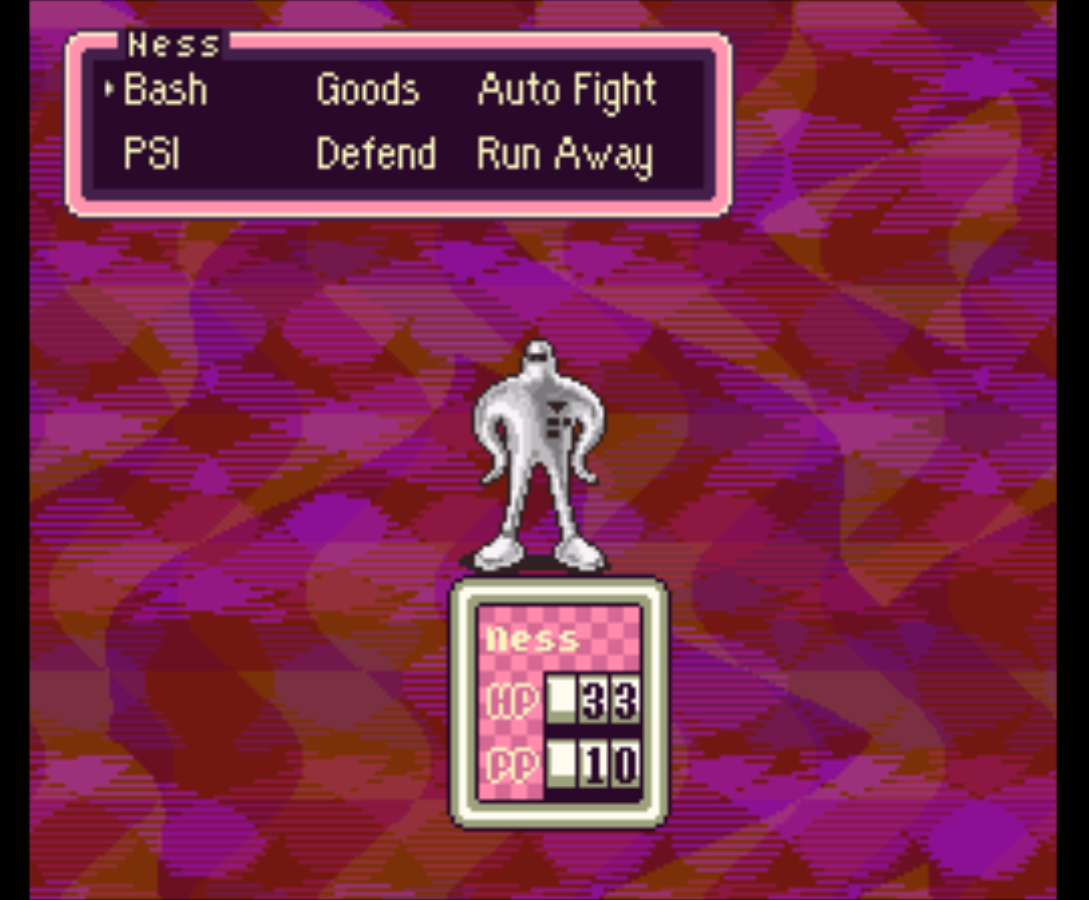
\includegraphics[width=9cm]{figures/Earthbound.png}
  \caption{A screenshot of a battle from the turn-based role-playing game \textit{Earthbound} \cite{earthbound94}.}
  \label{fig:Earthbound}
\end{figure}

For instance, observe the battle shown in Figure \ref{fig:Earthbound} from the game \textit{Earthbound}. The computer opponent is shown in the center of the screen. At the top, the actions available to the player are listed. Players have the choice of making a melee attack (Bash), casting a magical spell (PSI), using an item (Goods), or reducing damage taken (Defend). Players can also select Auto Fight to have the computer make all the choices for them, or they can Run Away and escape from the battle. At the bottom, the hit points (HP) and psychic points (PP) of the character are shown - these correspond to the character's health and their magical abilities.

Specific to turn-based RPGs, the player has as much time as they want to decide on their strategy. This is in contrast to an action RPG, where combat takes place in real-time. Generally, action RPGs use 3D environments to better accommodate the real-time battles, but this is not always the case. In the game created for this thesis, a turn-based approach is better suited because it emphasizes player strategy. Action RPGs may have similar lists of commands and actions, but these actions frequently have a corresponding skill component.\\

Take for example a basic attack. In a turn-based RPG, this action requires little from the player: they select that choice from a list, and their in-game character attacks the opposing player. Depending on the game, this attack may or may not be successful - the opponent could dodge or block the hit - but the success or failure is determined by the game through the stats of both players - if for instance a character has a high enough agility to dodge, or a high enough defensive to block the strike; the role-playing aspect of turn-based RPGs often boils down to how players build these stats. An action RPG, on the other hand, determines whether an attack misses or hits through hit-boxes. A hit-box is a hidden area tied to some in-game object; when hit-boxes intersect, something happens depending on the types of objects. For this example, an attack would be successful if the hit-box of the character's attack (their sword, fist, magic spell, etc.) intersects with the hit-box of their opponent's body. The attack would fail if these hit-boxes do not intersect. Thus, the overall success of a character in an action RPG is dependent on a player's skill in making hit-boxes collide. This type of gameplay does not lend itself well to game theory analysis, as a player could make all the right decisions but still lose from lack of skill.\\

\begin{figure}[H]
  \centering
  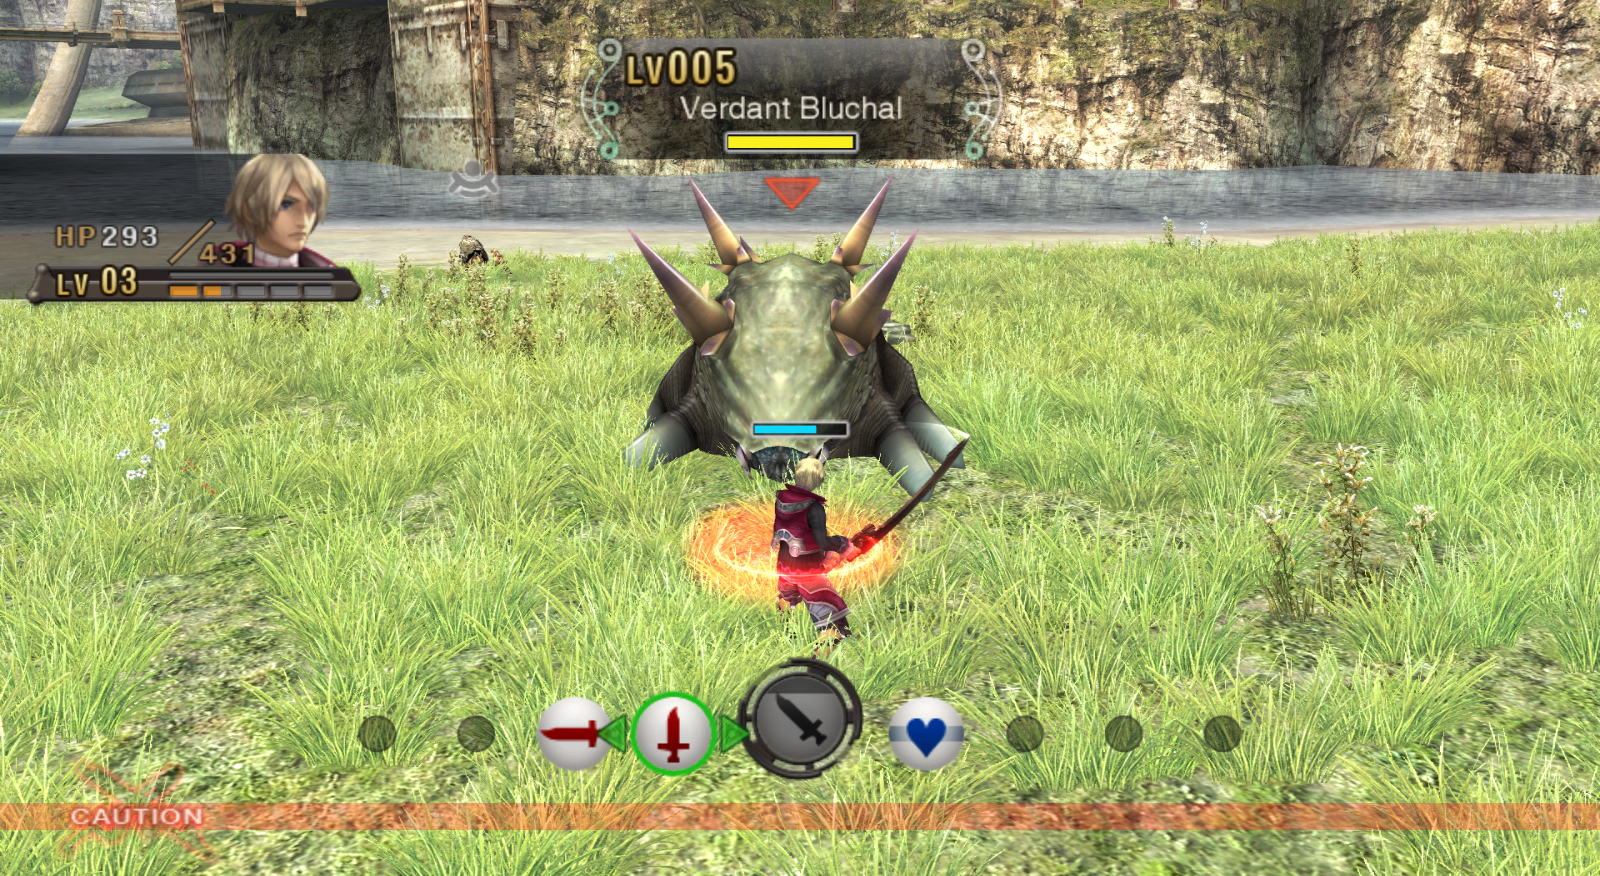
\includegraphics[width=9cm]{figures/Xenoblade.png}
  \caption{A screenshot of a battle from the action role-playing game \textit{Xenoblade Chronicles} \cite{xenoblade10}.}
  \label{fig:Xenoblade}
\end{figure}

For a more concrete example, regard a battle from the action RPG \textit{Xenoblade Chronicles}, as shown in Figure \ref{fig:Xenoblade}. In this game, the player can move freely in 3D space. The character shown has four abilities, represented as icons along the bottom of the screen. The two red-tinted abilities are attacks, as is the shaded center ability. The blue ability on the right is a healing spell. The skill component of this game comes with the two red abilities; these abilities do more damage and cause additional affects when performed at certain angles. For instance, the leftmost ability does more damage when used on an opponent's side, while the second red ability does more damage when used from an opponent's back. Thus, two players could use the same series of abilities but have different outcomes based on how their attacks were positioned.\\

Similarly, the game presented in this thesis is a two-dimensional game. With a turn-based RPG, since the gameplay involves choosing actions from a list, the only difference between a 2D and a 3D turn-based RPG is the graphical quality. A 2D game uses sprites, while 3D games use polygonal models. A two-dimensional game was chosen to simplify development.\\

To begin building an AI model, we first create a simulation of the \textit{Cave Escape}. The simulation has two players, each with 25 health points (HP). In this first simulation, both players have two possible actions per turn which are randomly selected: attack the other player, reducing their opponents HP by 5 points, or heal themselves, increasing their HP by 4 points. Players can not heal above their starting value of 25 HP; any extra health points are discarded. Each action has a 50\% chance of occurring. The game runs until one player's HP is reduced to 0. The total number of turns and the sequence of actions are recorded into a CSV file. After running 4500 simulations, the data is imported into MATLAB. A subset of the games are used as a training set for a decision tree, which predicts the player that wins the game.\\

\begin{figure}[H]
  \centering
  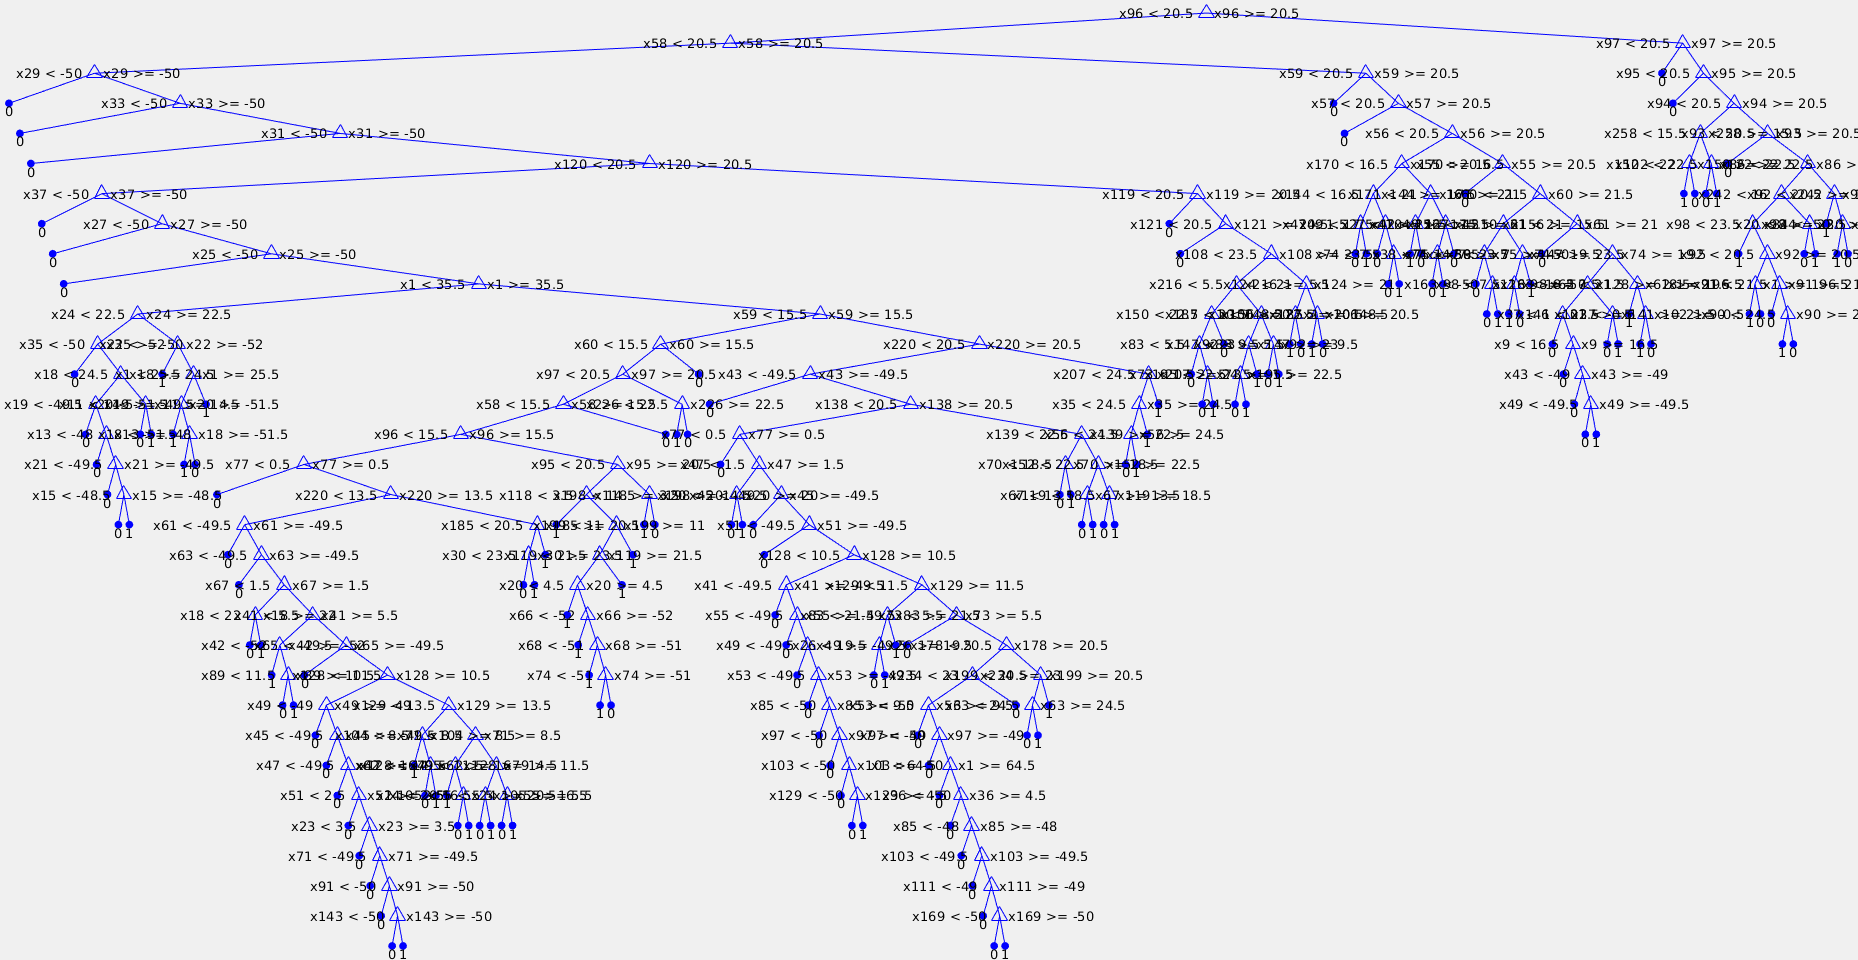
\includegraphics[width=13cm]{figures/firstDecisionTree.png}
  \caption{The decision tree generated from 4000 simulations of the game. The predicted attribute is a Boolean value of 0 when player 1 wins and 1 when player 2 wins.}
  \label{fig:decisionTree1}
\end{figure}

However, this method is inconclusive, for a number of reasons. Firstly, the decision tree includes a  large number of branches, as seen in Figure \ref{fig:decisionTree1}. Secondly, the actual criteria evaluated at each branch of the tree is different for each game. Aside from the first column, which contains the total number of turns in the game, and the second column, which contains the starting HP of player 1, the values in any particular column differ from game to game. For instance, the root node uses the value in column 96 as its classifier. In one game, column 96 may contain a HP value for player 2. In another, longer game, that column may contain a HP value for player 1. Thirdly, the individual games contain numerous streaks: a longer game is not the result of better strategy, but is instead caused by streaks where both players choose to heal on their turns. Players in these streaks reach HP levels near the 25 HP cap, effectively resetting the game.

The lack of consistency along columns is most likely the largest detriment to this model. Decision trees work best when classifying problems on specific attributes; if the attribute is different at column 96 from one game to another, the information gain at that column is meaningless. This is likely behind the sprawling nature of the decision tree itself. Without clear attributes to test, each split only has minuscule amounts of information gain.

\subsection{Extensive Tree Model}
A game theoretic angle is used on the second attempt. The HP of both players is reduced to 10, and two restrictions are added on healing: a player can not heal when they have full health, and a player can only heal themselves twice. As in the first attempt, players can only attack or heal. With these new rules in place, we create an extensive-form tree for the new game.\\

\begin{figure}[H]
  \centering
  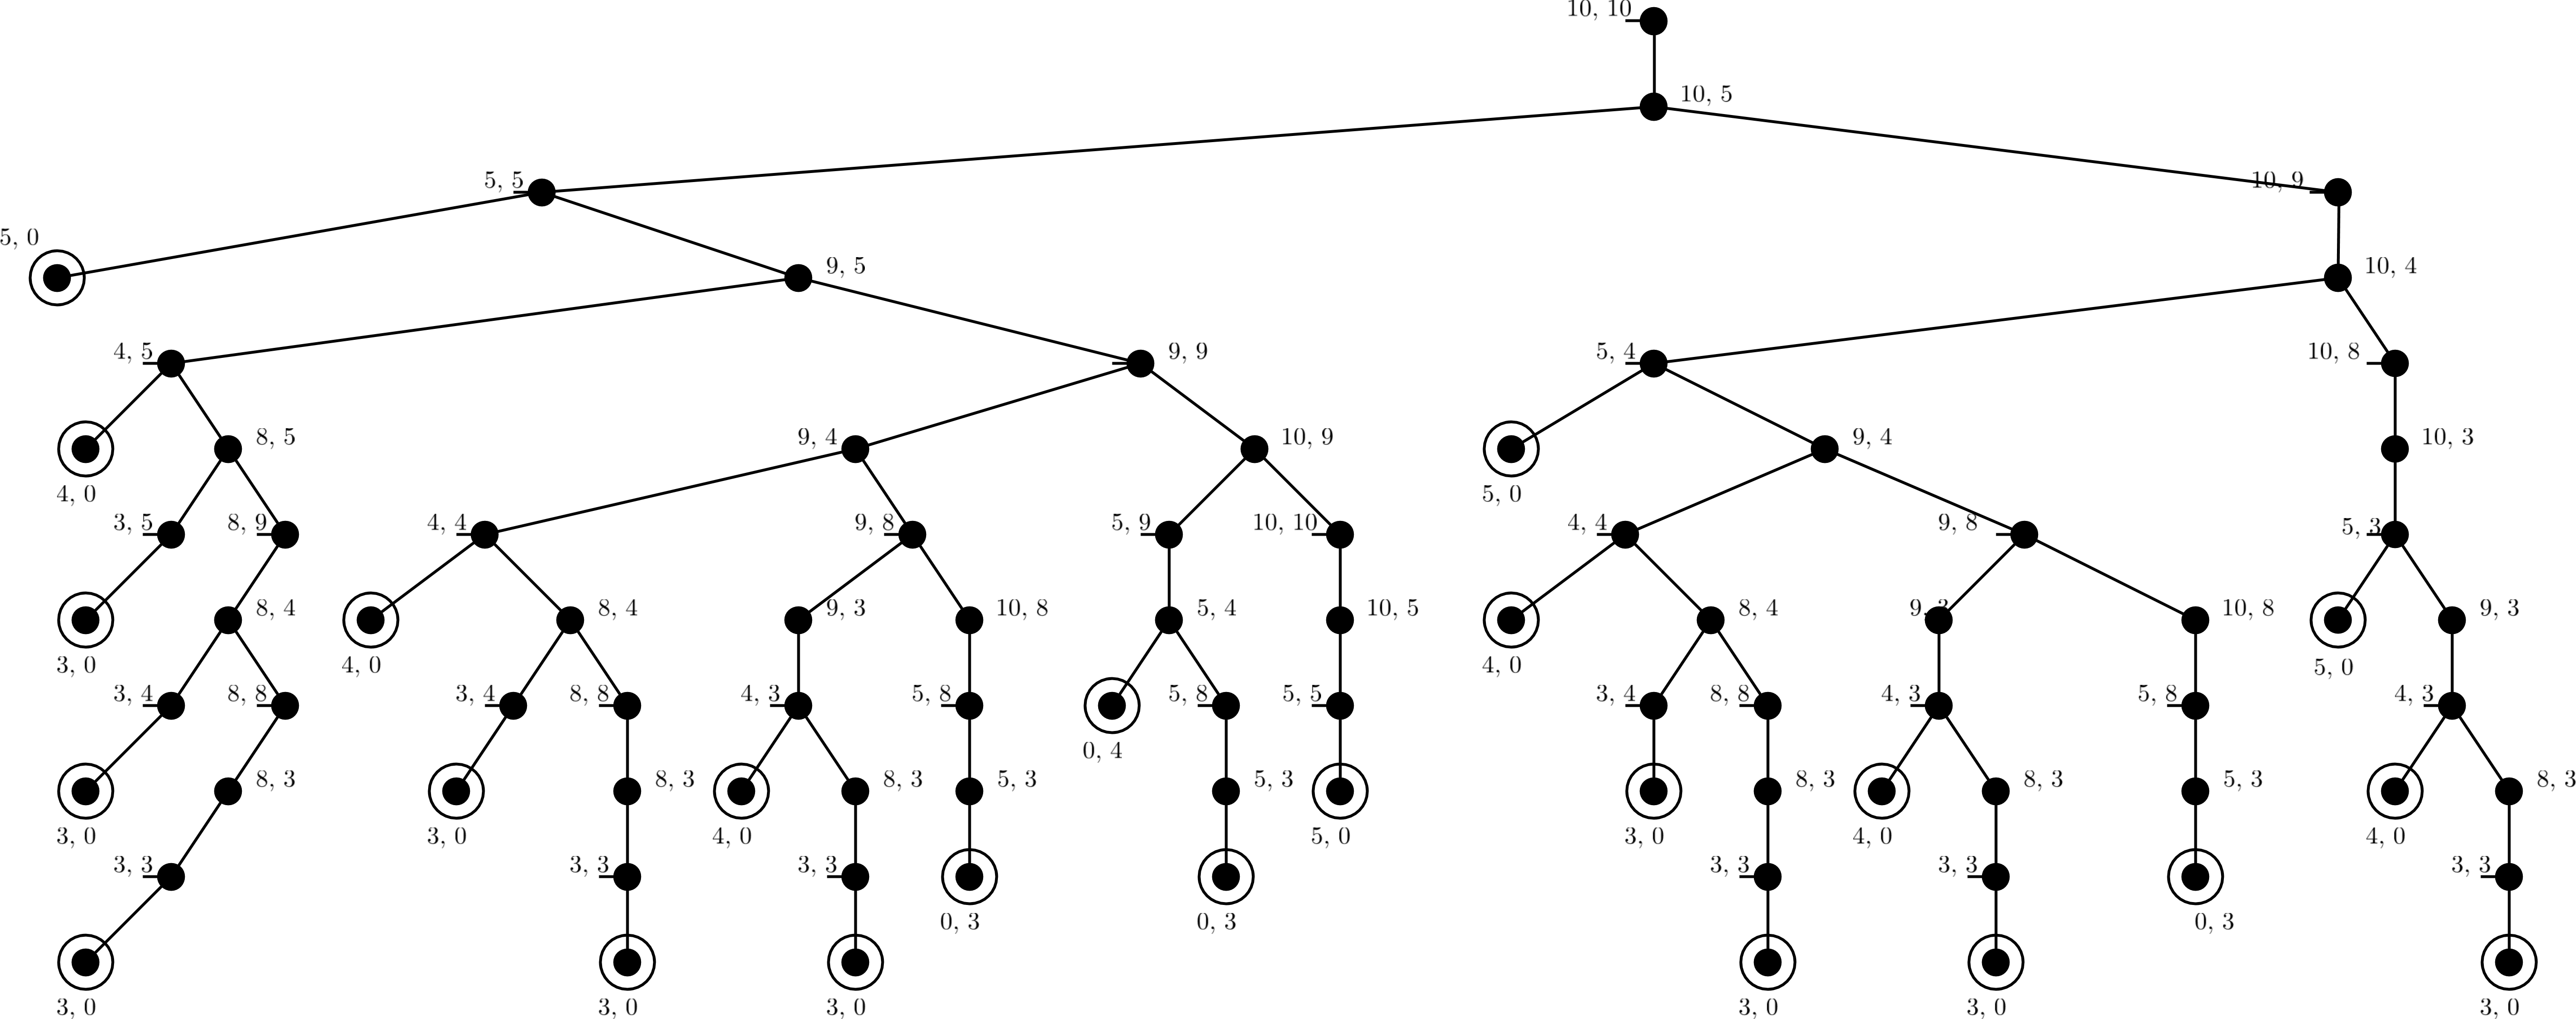
\includegraphics[width=15cm]{figures/GameTree.png}
  \caption{The extensive-form tree for a simplified game. Each player starts with 10 hit points (HP). At each node, a player can choose to heal themselves or attack their opponent. Attacking reduces the opponent's HP by 5 points. Healing increases the decision maker's HP by 4 points; they can only heal themselves twice per game.}
  \label{fig:gameTree}
\end{figure}

In Figure \ref{fig:gameTree}, player 1's nodes are denoted by a small dash to the left of the node. The HP values of both players are recorded at each node. Leaf nodes where player 1 wins are enclosed in a circle, and leaf nodes where player 2 wins are enclosed in a diamond. There are 24 outcomes for this game; of these, only 4 of them result in a win for player 2, while the other 20 result in wins for player 1. In fact, with optimal play, player 1 always wins in this game.\\

\begin{figure}[H]
  \centering
  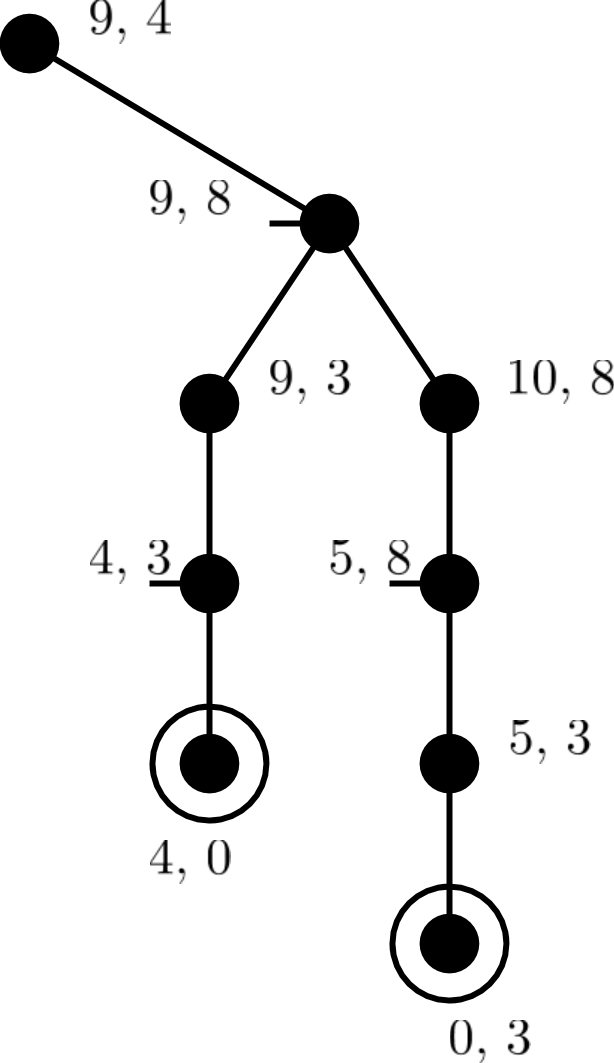
\includegraphics[width=4cm]{figures/GameSubtree.png}
  \caption{A subtree of the extensive-form representation in Figure \ref{fig:gameTree}. This subtree contains one of player 2's only winning outcomes.}
  \label{fig:gameSubtree}
\end{figure}

For example, in the subtree shown in Figure \ref{fig:gameSubtree}, both player 1 and 2 have a winning outcome. However, the critical decision is made by player 1. If player 1 chooses to heal, then player 2 will win in 3 more turns. If player 1 chooses to attack, then player 1 will eventually win. Thus, in any game which reaches this subtree, player 1 chooses to attack on their turn, since that choice leads to their victory.\\

\begin{figure}[H]
  \centering
  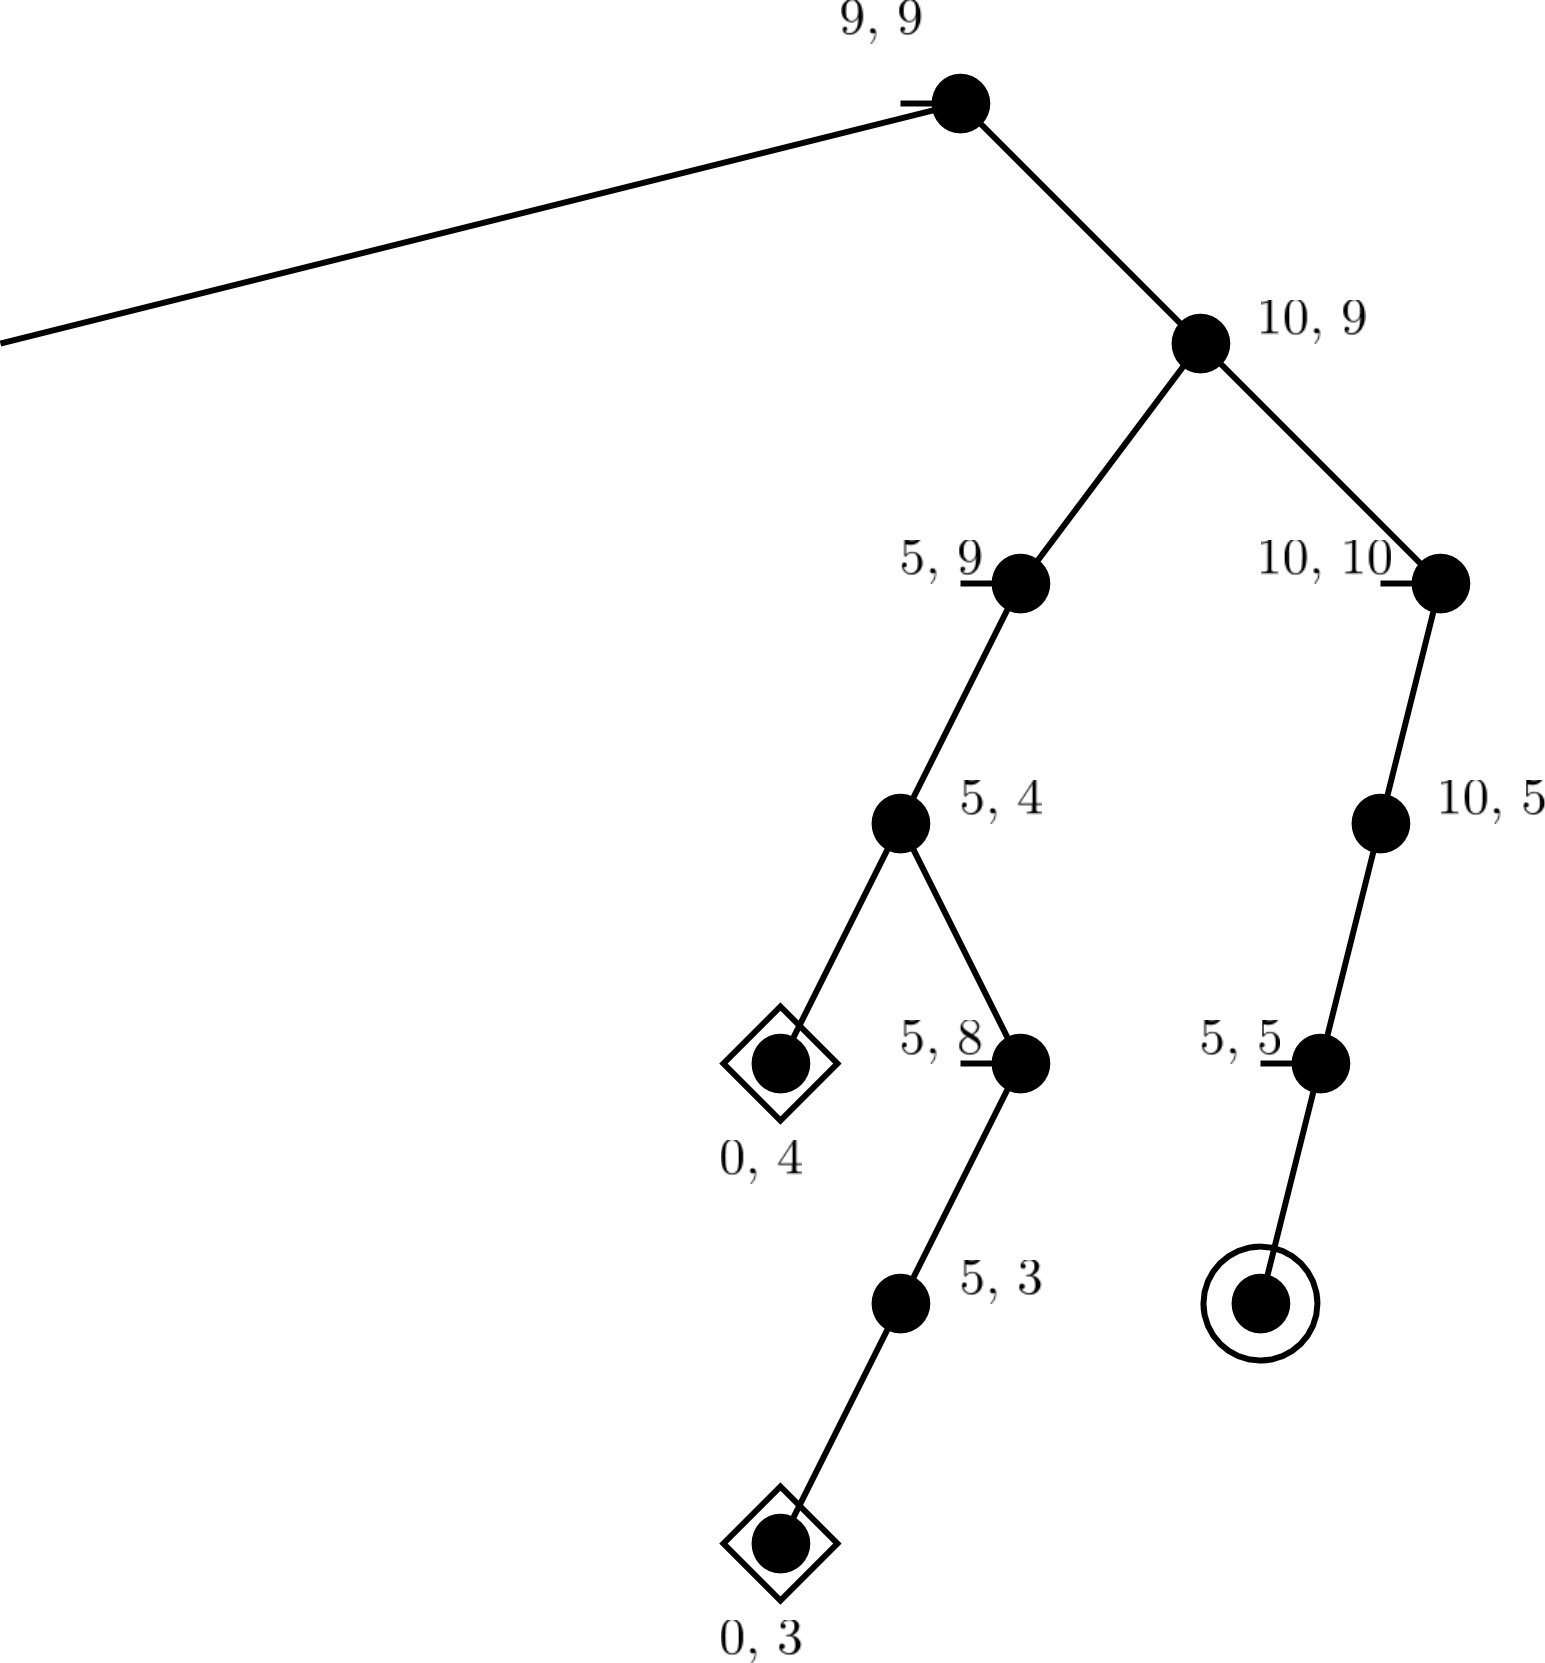
\includegraphics[width=8cm]{figures/GameSubtree2.png}
  \caption{A second subtree of the extensive-form representation in Figure \ref{fig:gameTree}. This subtree contains two more of player 2's winning outcomes.}
  \label{fig:gameSubtree2}
\end{figure}

Two more of player 2's winning outcomes can be seen in the subtree in Figure \ref{fig:gameSubtree2}. At the root node of this subtree, player 1 is making their choice. If they choose to heal, the game moves into the right child. Player 2's first choice on the right child's subtree either results in a win (if player 2 attacks) or a loss (if player 2 heals). Thus, an intelligent player 2 would always attack at this stage, since it is a guaranteed win. However, if player 1 knows that this is a guaranteed win for their opponent, player 1 can avoid this threat by attacking instead of healing at the root node.\\

If player 1 decides to avoid the subtree in Figure \ref{fig:gameSubtree2}, player 2 has the next choice. If player 2 decides to heal at this new node, then the resulting subtree is identical to the one found in Figure \ref{fig:gameSubtree}. This subtree contains player 2's final winning outcome, but once again player 1 can avoid this outcome with ease.\\

\subsubsection{Backwards Induction on Extensive Tree Model}
We can prove that player 1 will always win this game through the backwards induction algorithm discussed in Chapter 2. Recall that the algorithm travels through a game tree by recursion and, at each node, returns the child node which gives the player acting at the parent node the most utility.

\begin{figure}[H]
  \centering
  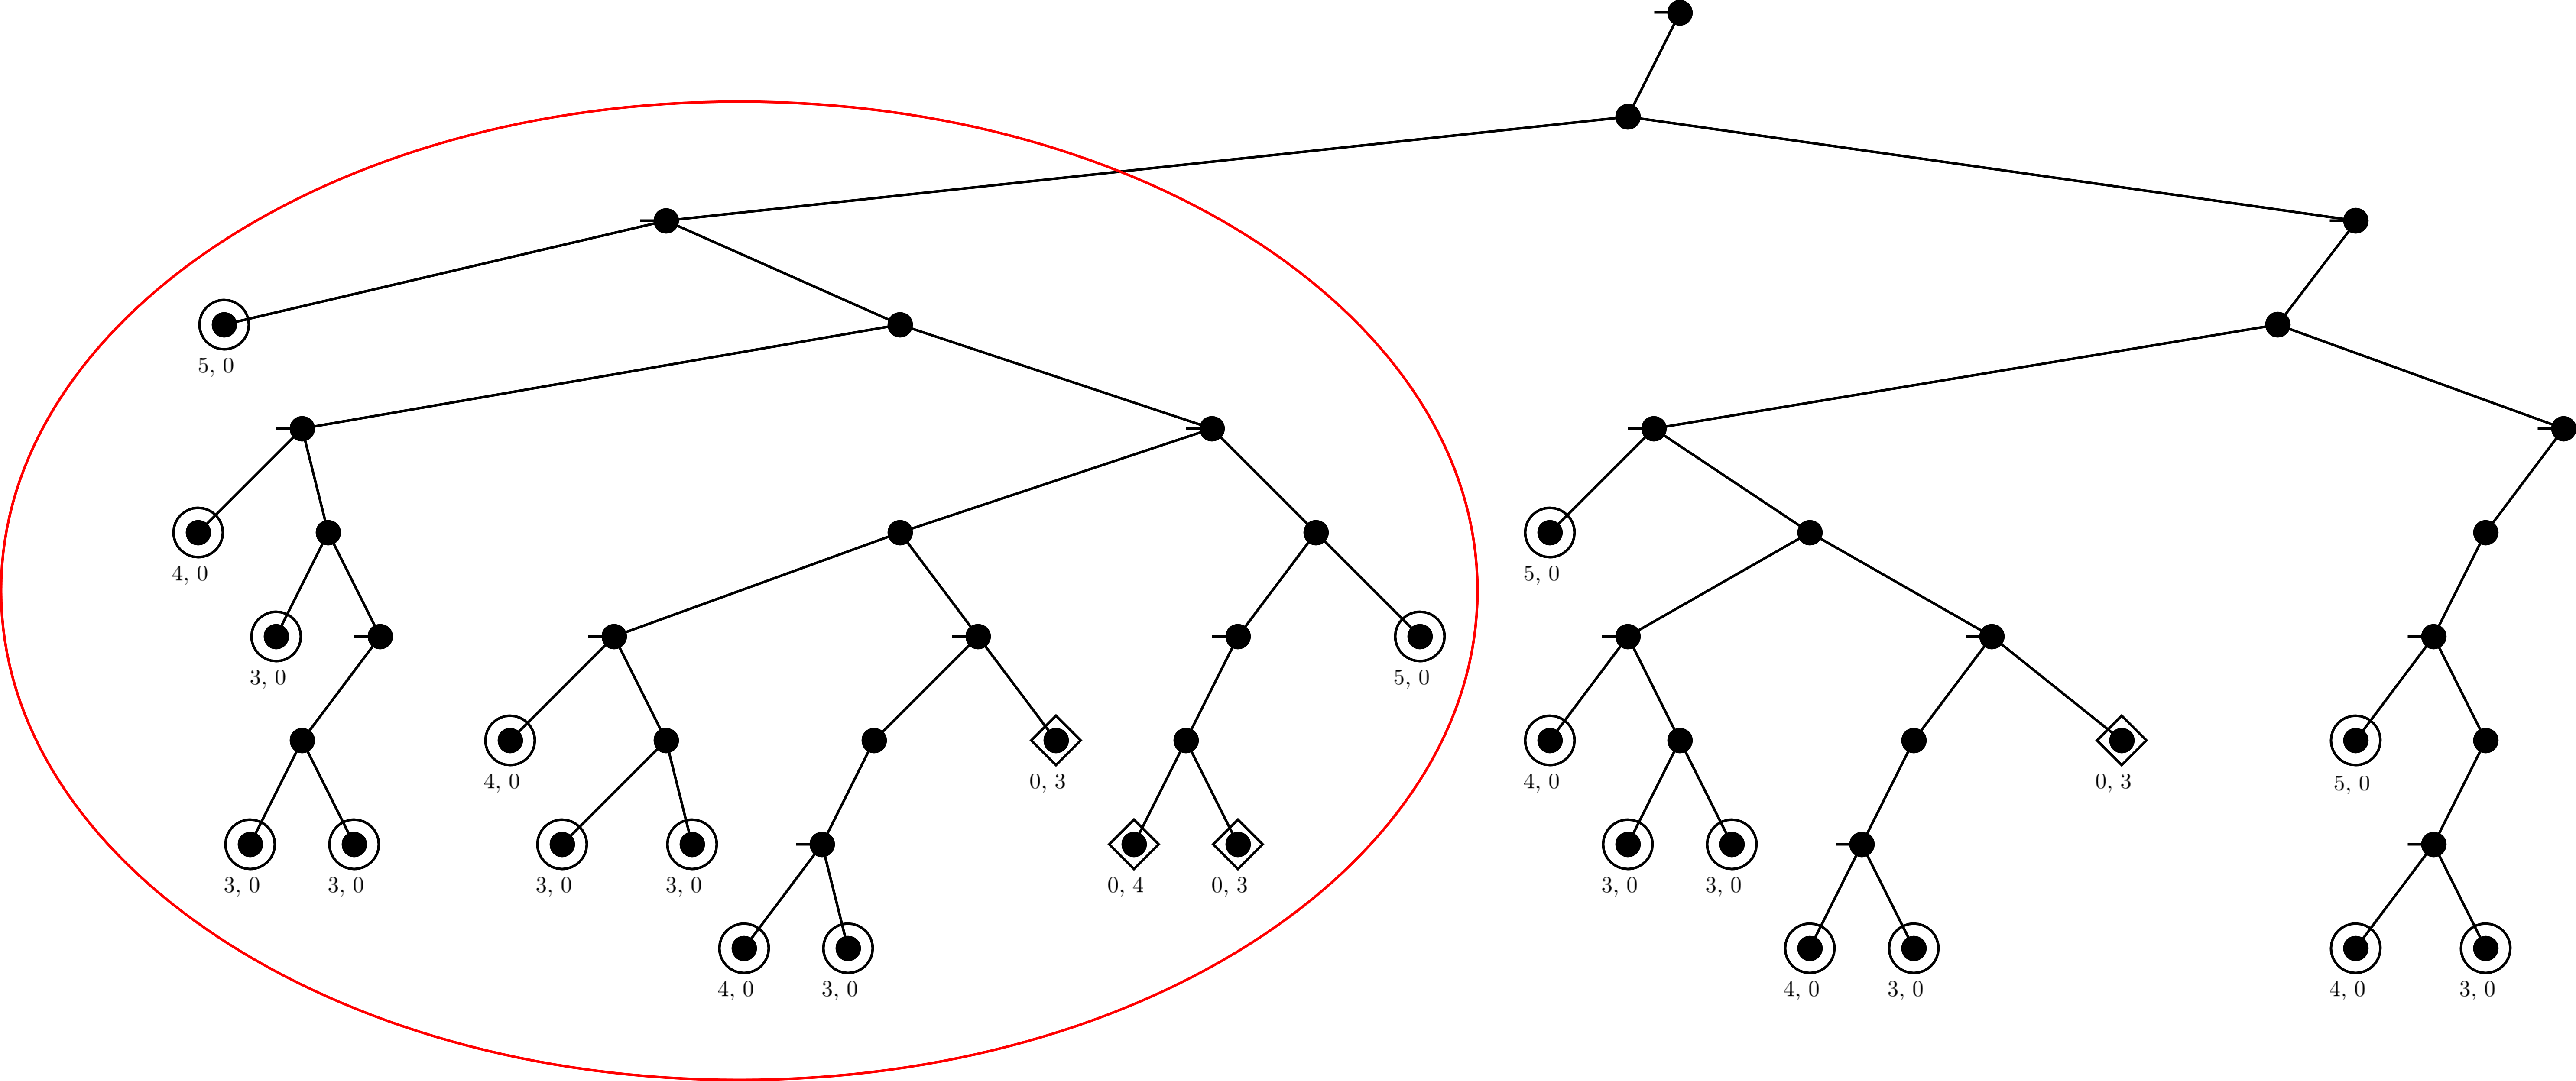
\includegraphics[width=15cm]{figures/Backwards0.png}
  \caption{The extensive-form tree for the simplified version of the game, but with extraneous nodes removed; a node is extraneous if the player making their decision has only one possible action. The circled subtree will be the first subtree examined on recursive calls of the backwards induction algorithm.}
  \label{fig:condensedTree}
\end{figure}

For the example in Figure \ref{fig:gameTree}, we can trivially condense branches where only one action is available, taking the utility values from the leaf nodes and copying them up the tree. This produces the tree seen in Figure \ref{fig:condensedTree}. We define the utility of a player in this game as their HP at the end of the game minus the HP of their opponent. Thus, for a game with the outcome (4, 0), player 1 will have a utility of 4 and player 2 will have a utility of -4.\\

The algorithm begins at the root node of the tree. Since the root is not a leaf node, the algorithm is called on the root's children, starting with the leftmost child. The root node only has one child, since players cannot heal when their HP is maxed out. So, the backwards induction algorithm is called on the next node, which does have more than one child. To find the utility of both children, the algorithm must be recursively called on both subtrees, starting with the subtree circled in red in Figure \ref{fig:condensedTree}.\\

\begin{figure}[H]
  \centering
  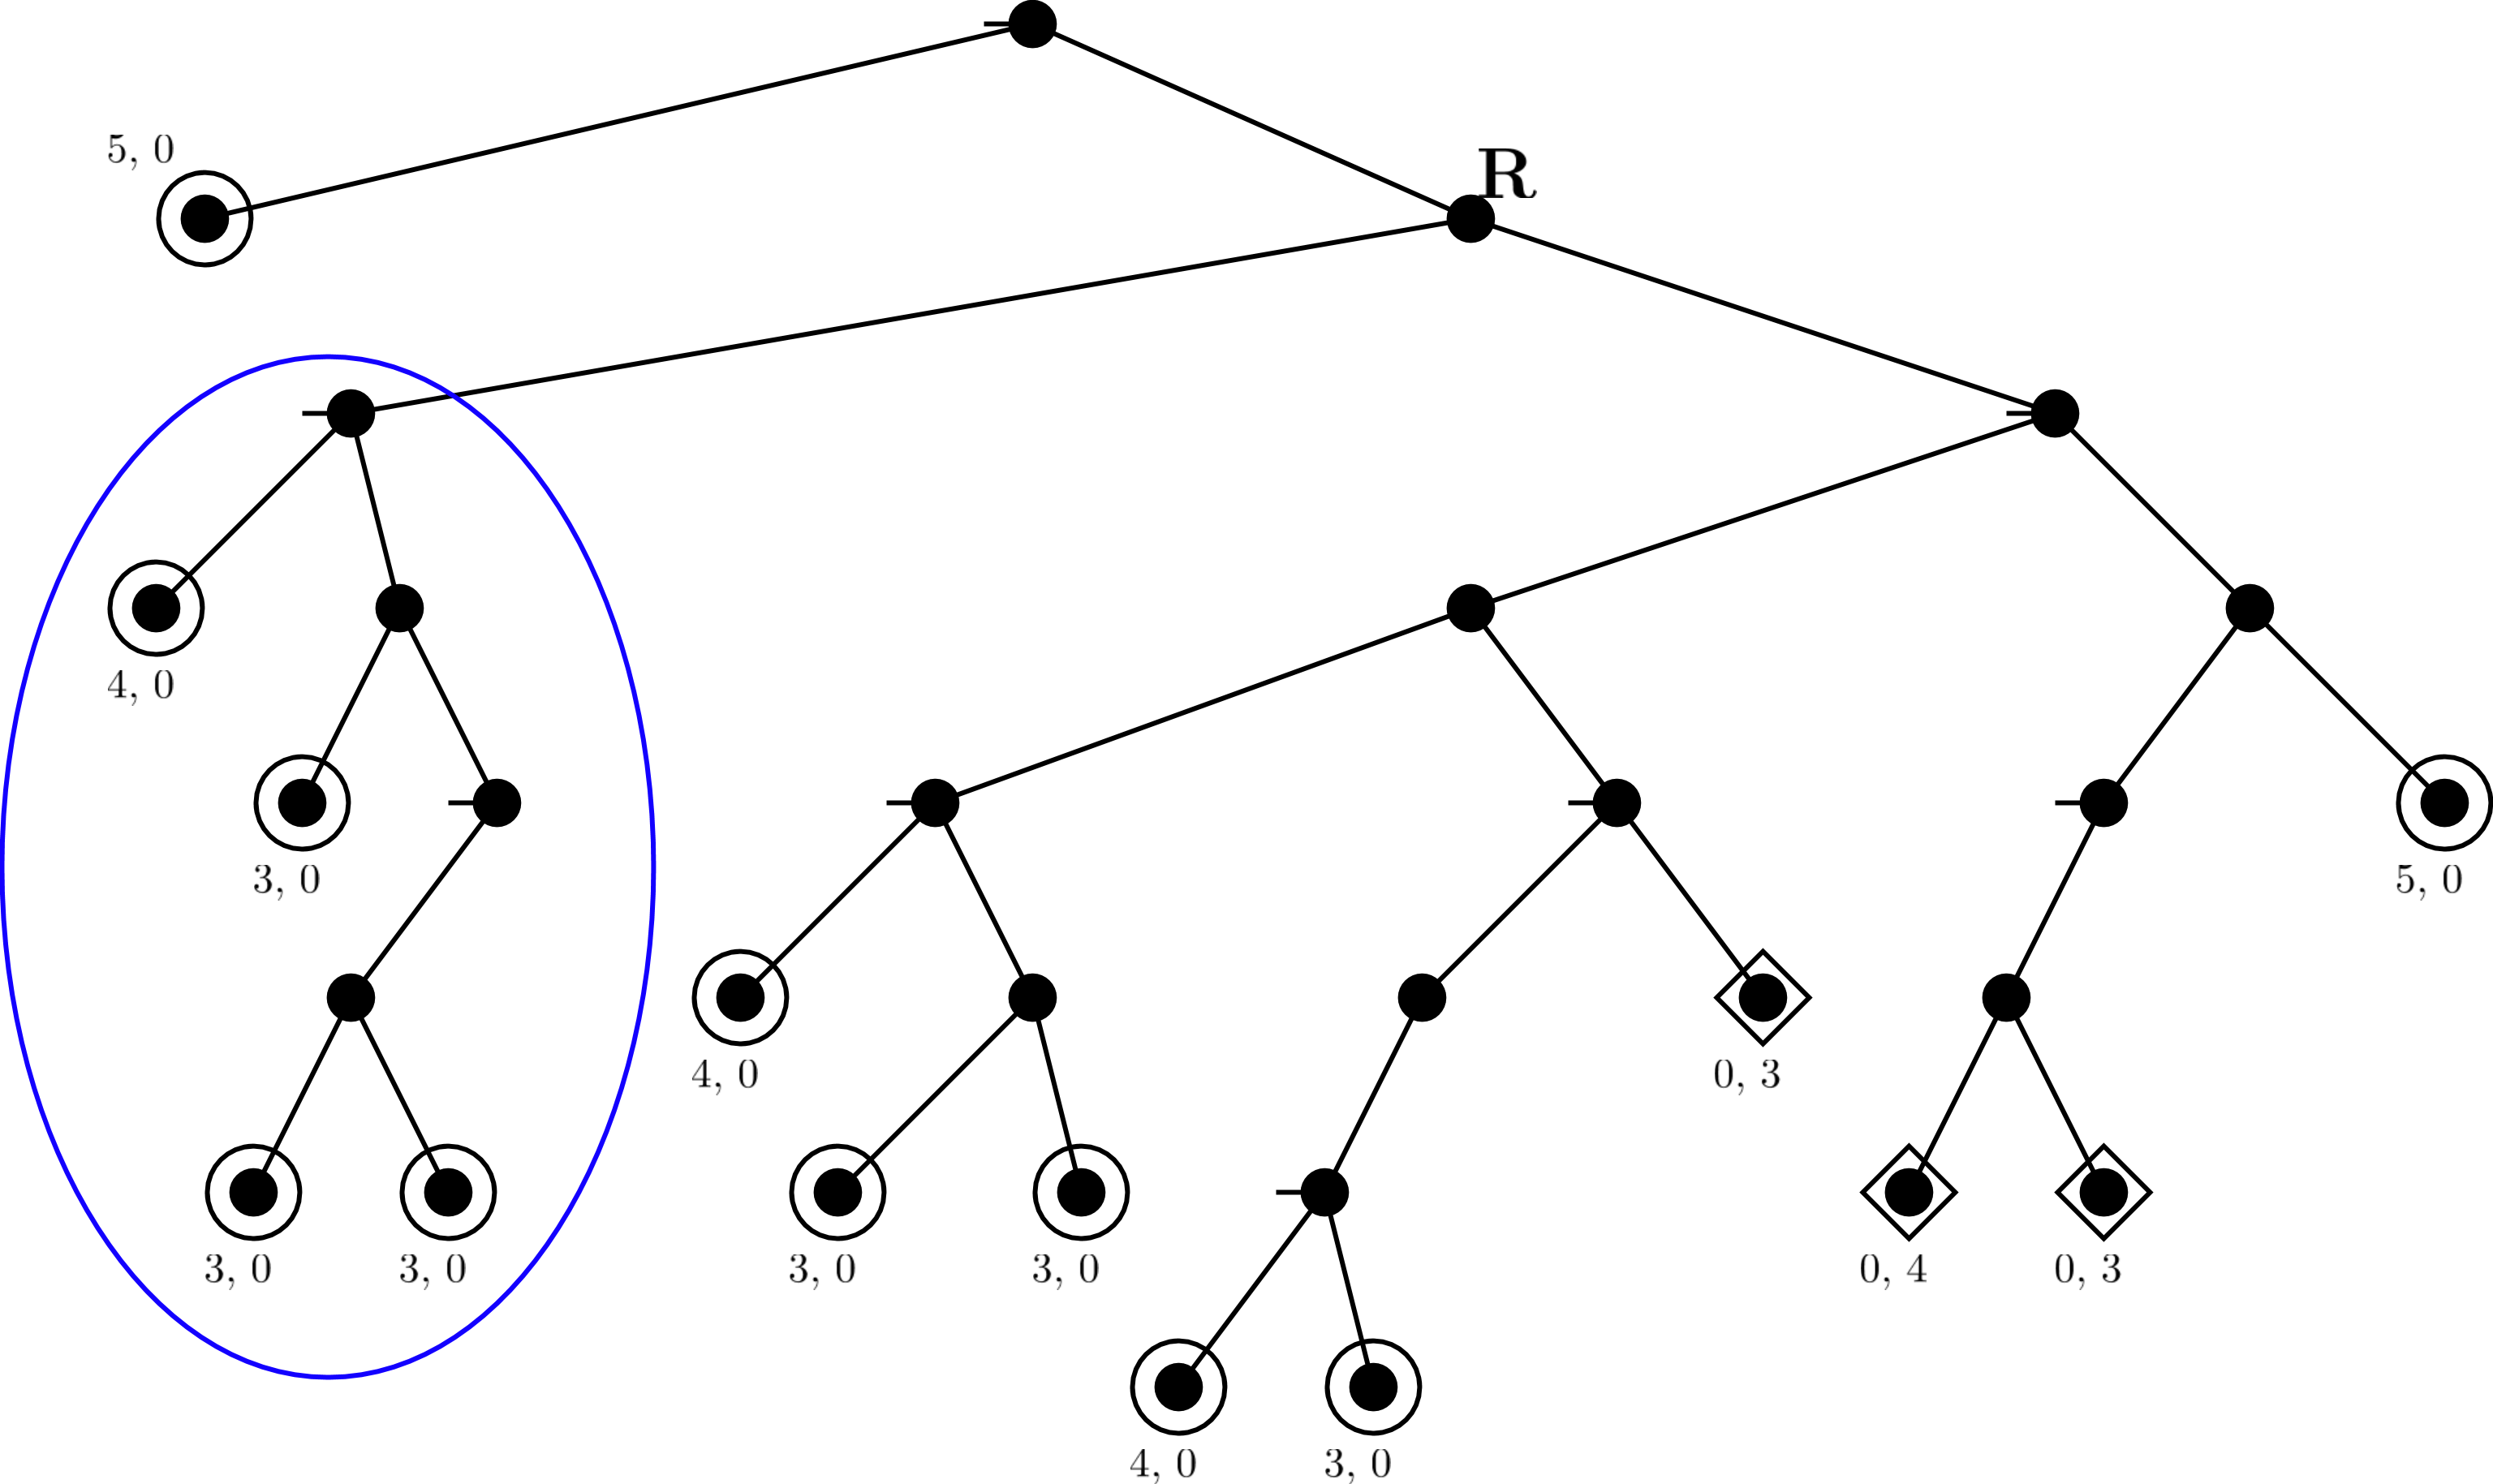
\includegraphics[width=11cm]{figures/Backwards1.png}
  \caption{The tree examined by the backwards induction algorithm after recursing to the red circled subtree in Figure \ref{fig:condensedTree}. The blue circled subtree is the next recursive step of the algorithm.}
  \label{fig:backwards1}
\end{figure}
Examining the root of the subtree in Figure \ref{fig:backwards1}, we find that the left child of the root is a leaf node. Thus, since the root is a decision node for player 1, the utility of this entire subtree will be the maximum utility for player 1 between the leaf node (5, 0) and the utility of the right child, which is its own subtree. Once again, the backwards induction algorithm is called recursively, this time on the subtree with root $R$. On the recursive call, the left child of $R$ is the subtree circled in blue.\\

\begin{figure}[H]
  \centering
  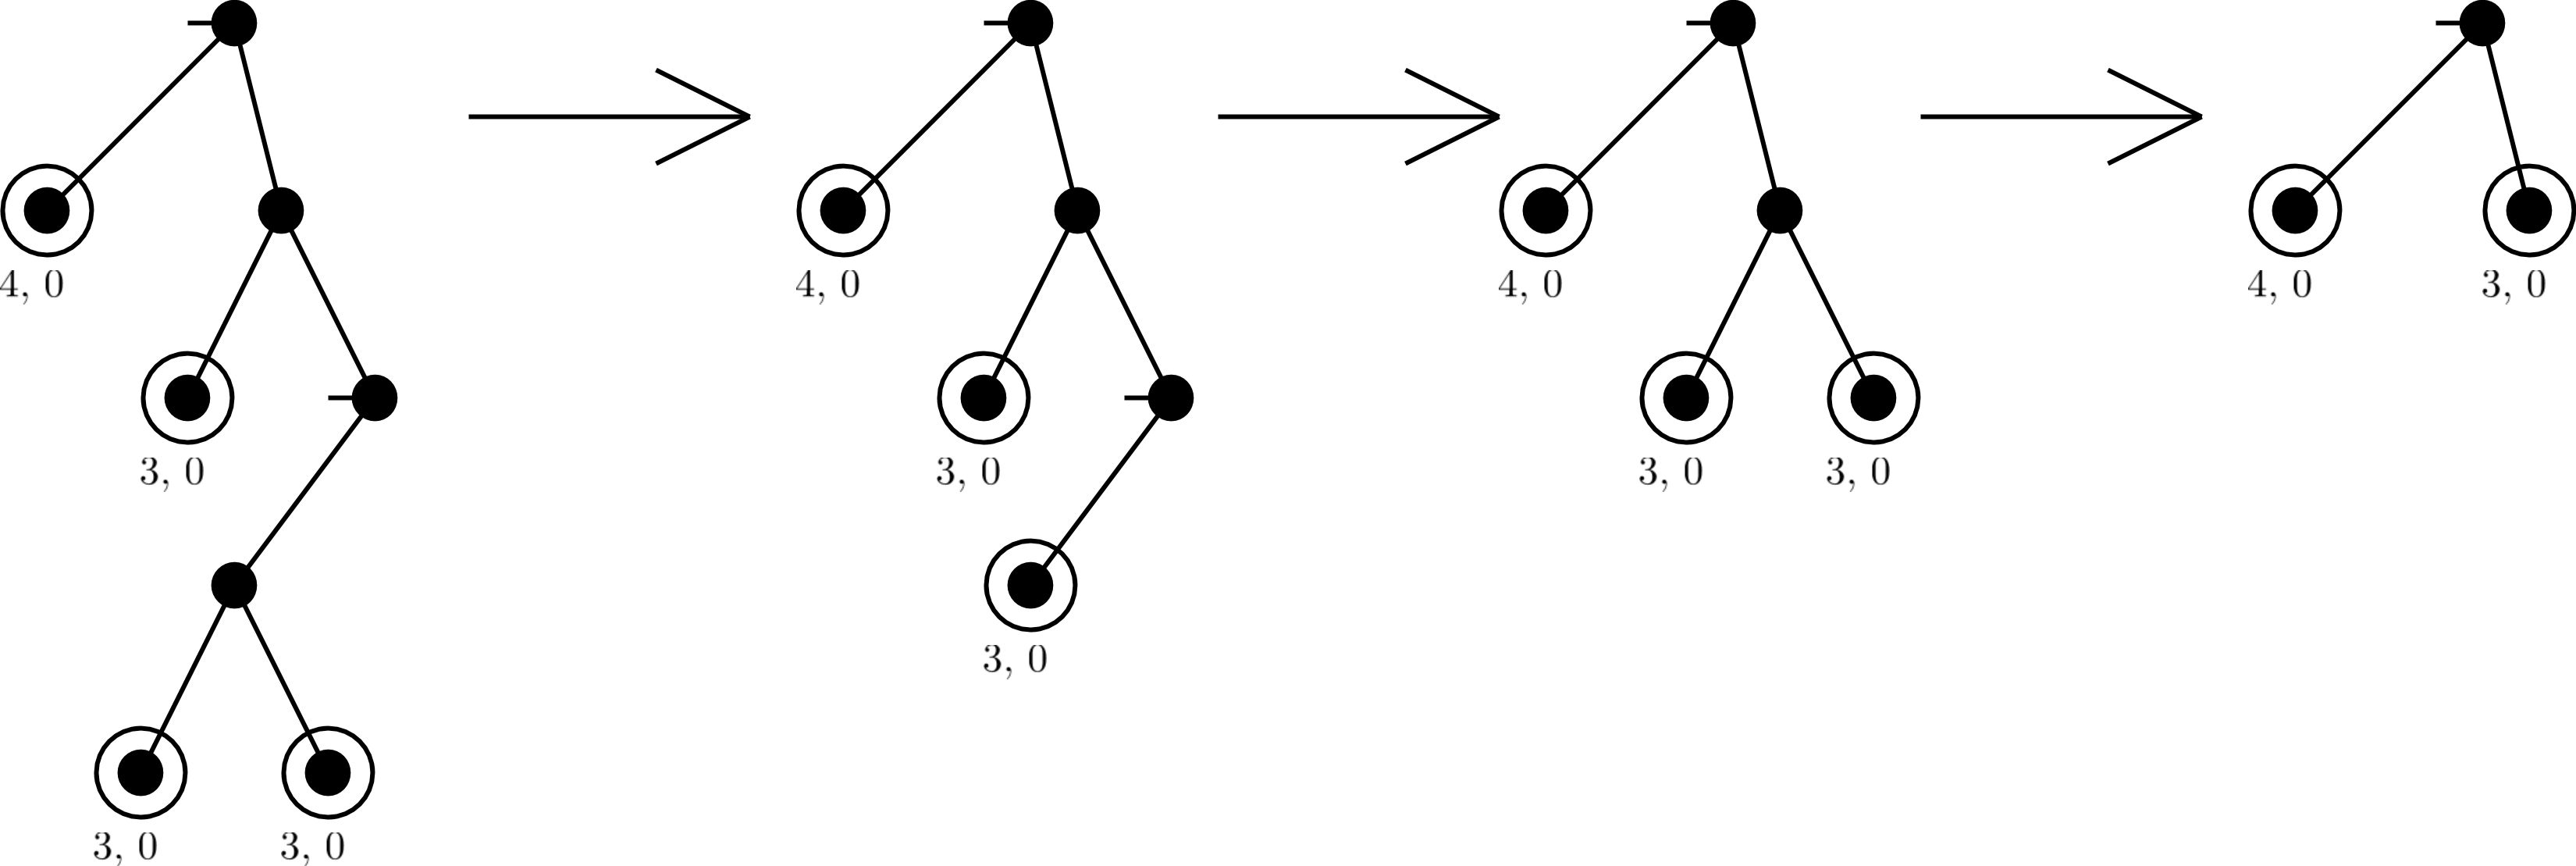
\includegraphics[width=12cm]{figures/Backwards2.png}
  \caption{The steps taken by the backwards induction algorithm after reaching the circled subtree in Figure \ref{fig:backwards1}.}
  \label{fig:backwards2}
\end{figure}
As the algorithm continues to recurse through the game tree, it will eventually reach the pair of leaf nodes at the bottom of the leftmost tree in Figure \ref{fig:backwards2}. The preceding decision node is a choice for player 2, so player 2 will make whichever choice gives them more utility. In this example, both leaf nodes provide player 2 with -3 utility, so the utility of the decision node is (3, 0). This utility value is moved up the tree to the next decision node, as shown in Figure \ref{fig:backwards2}. These steps continue up the subtree. The next decision node again has a tie between (3, 0) and (3, 0), but the root of the subtree has a choice between (3, 0) and (4, 0). Since the root of this subtree is a decision node for player 1, that player will prefer to attack and reach the (4, 0) leaf node for 4 utility. Thus, the utility of the circled subtree in Figure \ref{fig:backwards1} is (4, 0).\\

\begin{figure}[H]
  \centering
  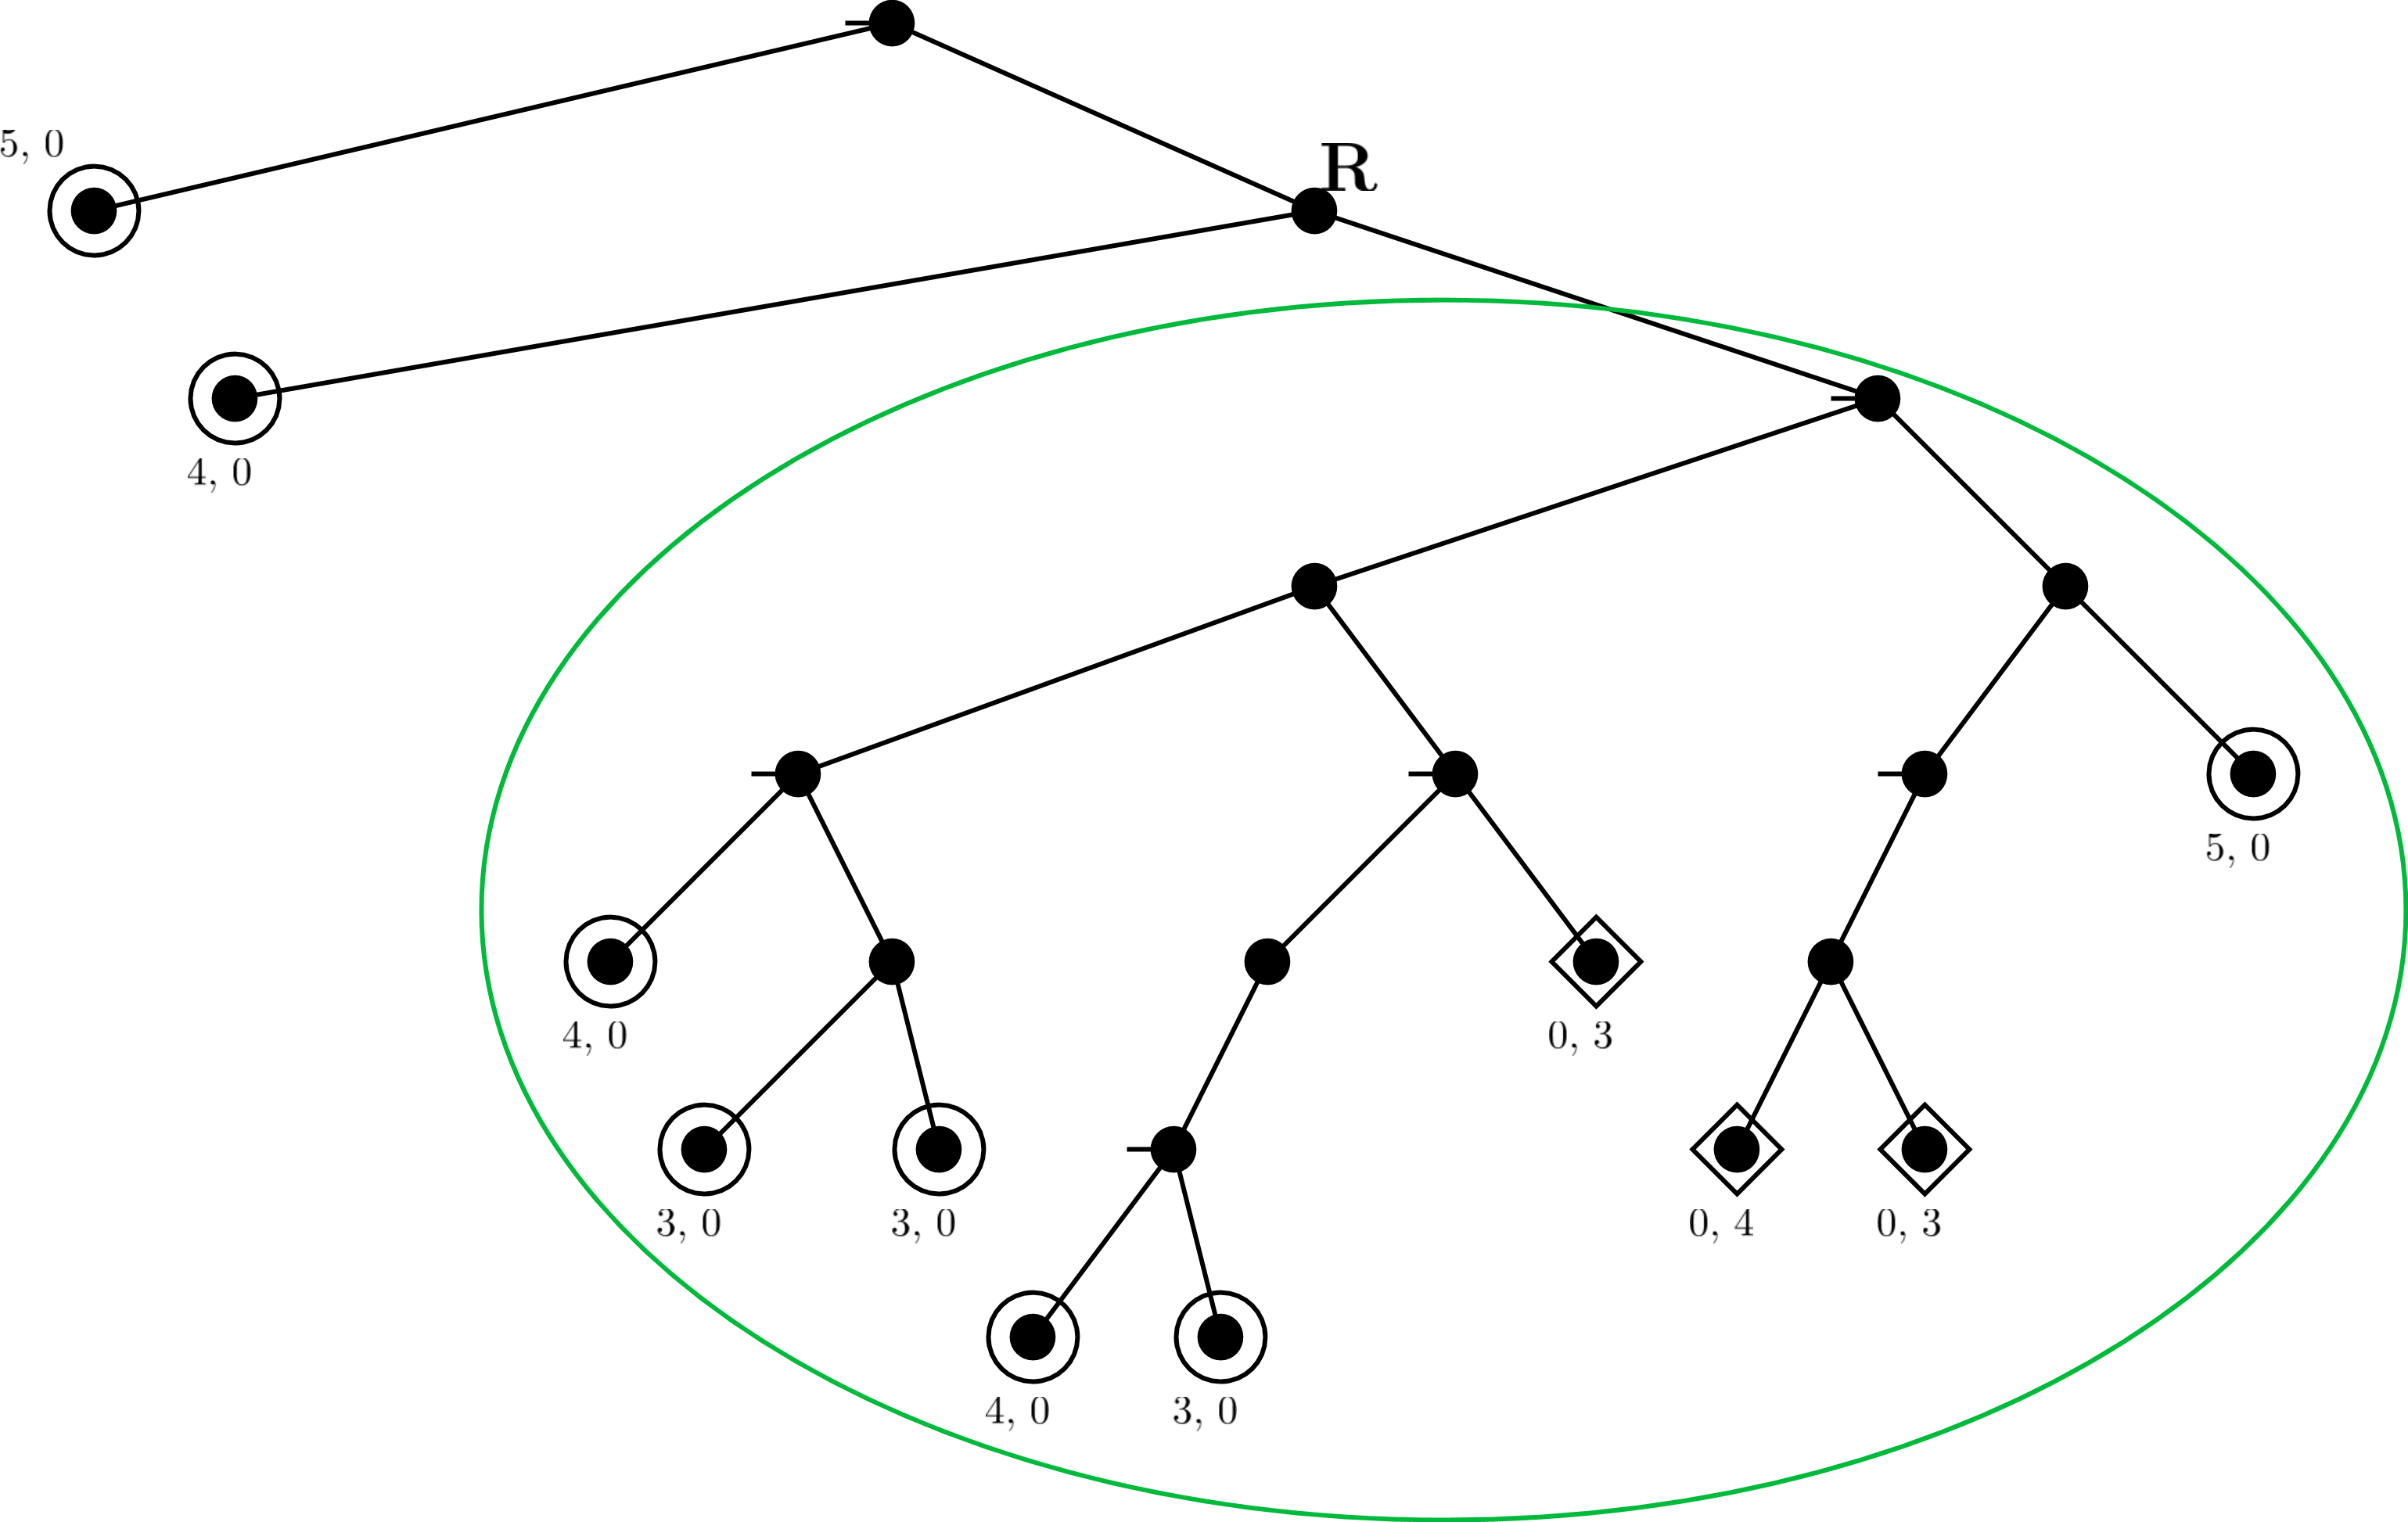
\includegraphics[width=11cm]{figures/Backwards3.png}
  \caption{The subtree in Figure \ref{fig:backwards1}, after the backwards induction steps performed in Figure \ref{fig:backwards2}.}
  \label{fig:backwards3}
\end{figure}

Thus, after exploring the subtree in Figure \ref{fig:backwards2}, the left child of node $R$ is changed from a subtree to a single leaf node, the leaf with utility (4, 0). Now that the left child of $R$ is a leaf node, the algorithm continues along the right subtree of $R$, circled in green.\\

\begin{figure}[H]
  \centering
  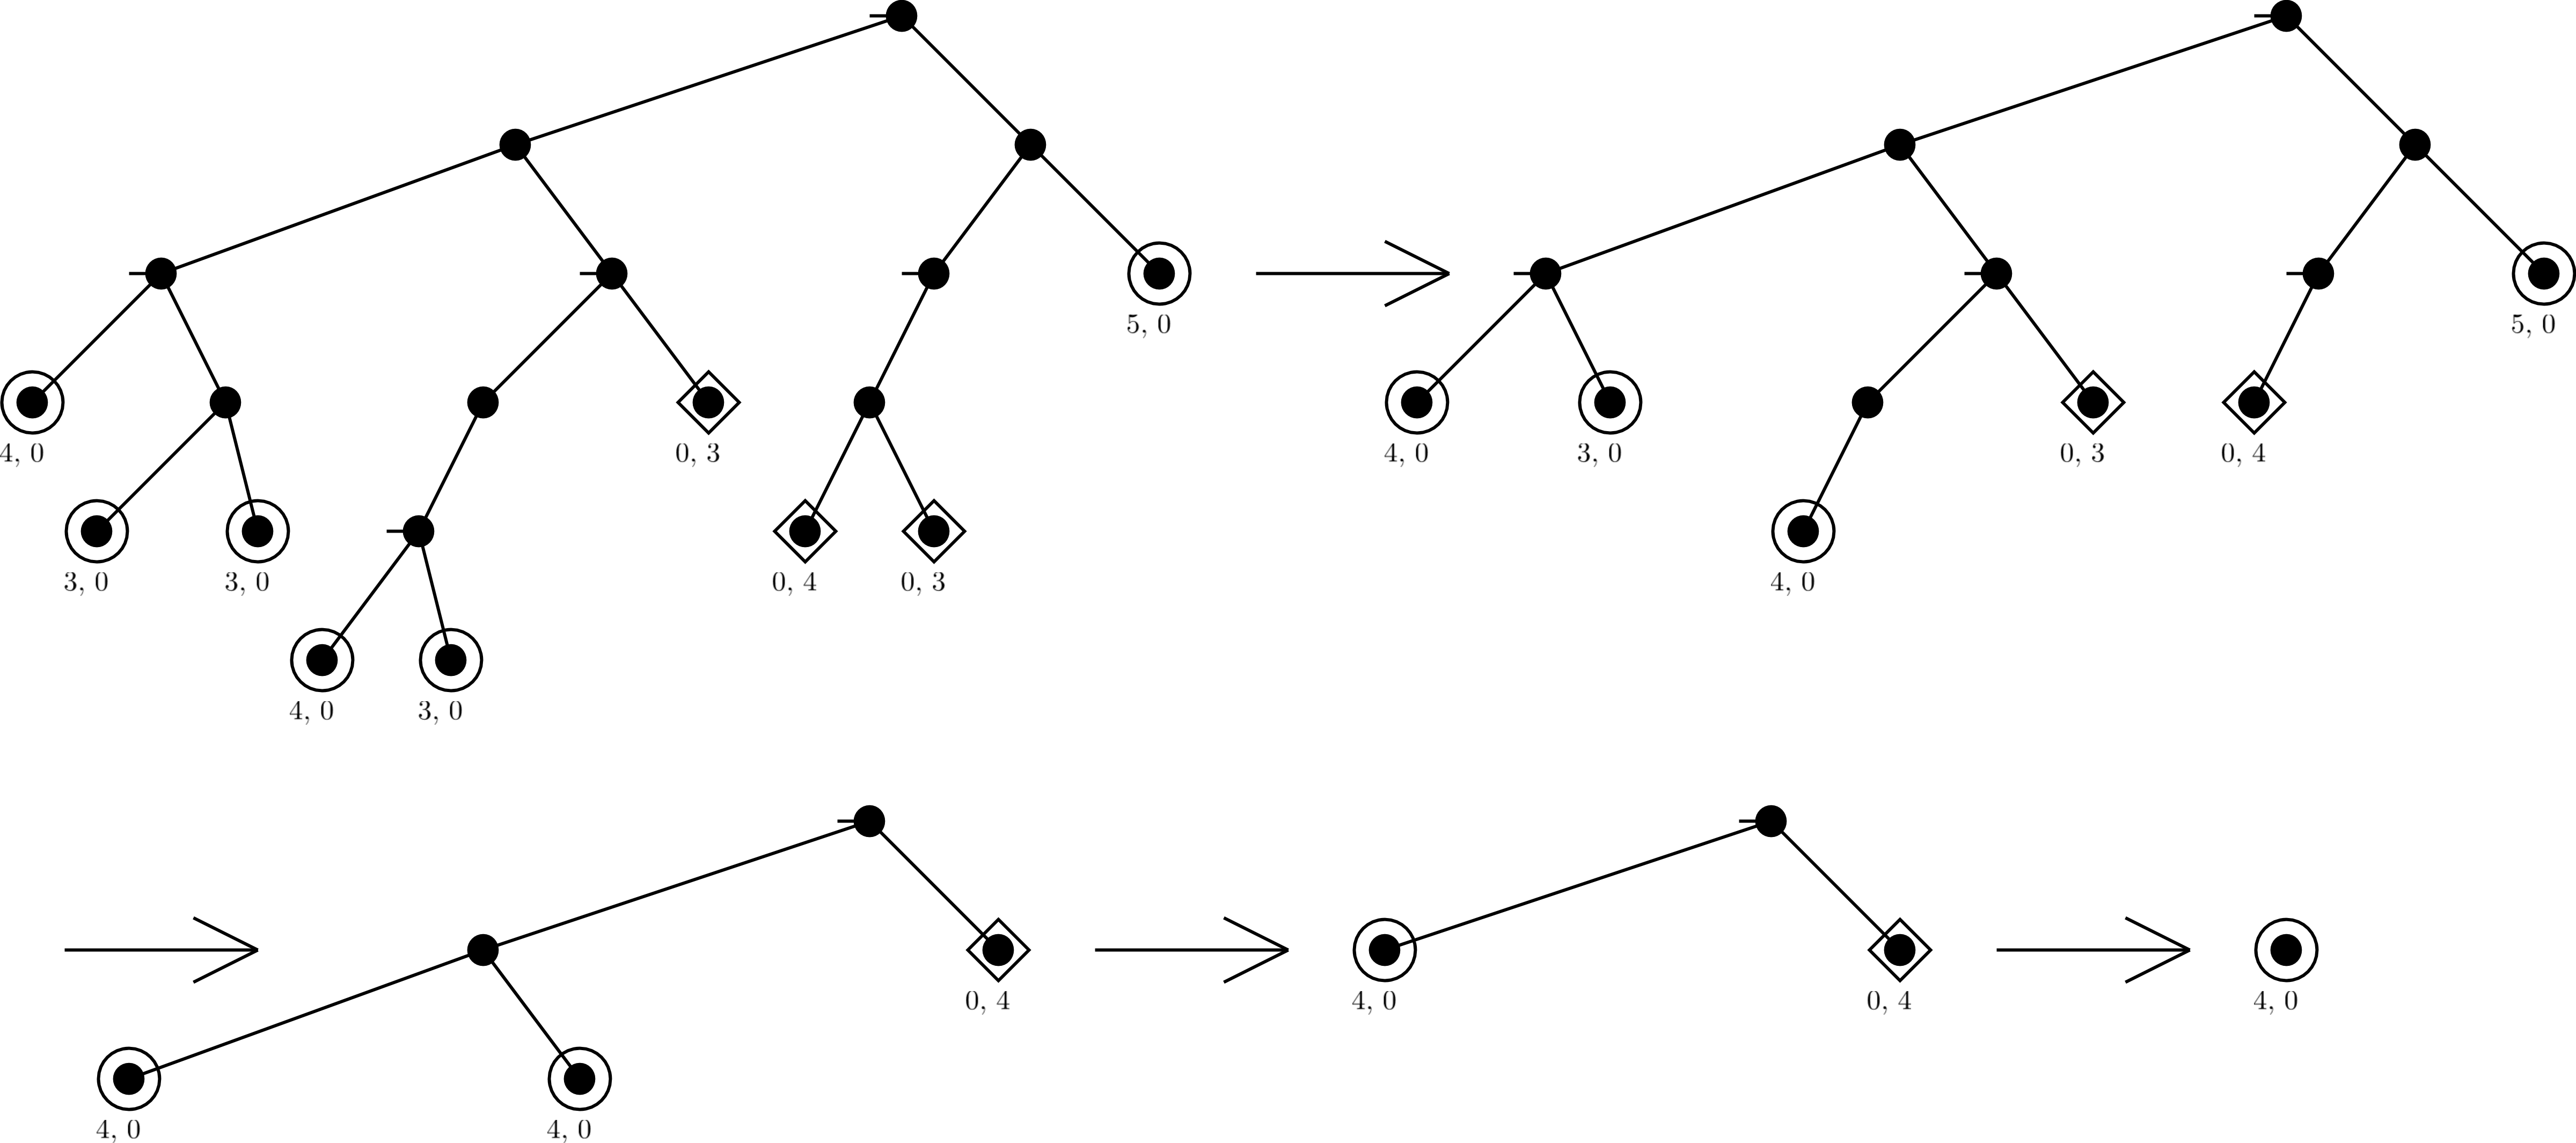
\includegraphics[width=14cm]{figures/Backwards4.png}
  \caption{The steps taken by the backwards induction algorithm after reaching the circled subtree in Figure \ref{fig:backwards3}.}
  \label{fig:backwards4}
\end{figure}

In the new subtree, the induction algorithm again determines which of the leaf nodes to bring up the tree. The parent of the leaf nodes decides which leaf provides the most utility for that player. In the first step, along the bottom of the tree and from the left, player 2 makes a choice between (3, 0) and (3, 0); player 1 makes a choice between (4,0) and (3, 0); player 2 makes a choice between (0, 4) and (0, 3). Respectively, the algorithm chooses (3, 0), (4, 0), and (0, 4). Each of these best leaf nodes are moved up the tree, resulting in the second tree in Figure \ref{fig:backwards4}. From here, extraneous branches are removed and three more decisions are made: player 1 chooses between (4, 0) and (3, 0); player 1 chooses between (4, 0) and (0, 3); player 2 chooses between (0, 4) and (5, 0). Respectively, the new utilities of the decision nodes are (4, 0), (4, 0), and (0, 4), creating the third tree in Figure \ref{fig:backwards4}. The next decision is made by Player 2, and is a tie between the two (4, 0) nodes. Then, in the fourth tree shown in Figure \ref{fig:backwards4}, Player 1 makes their choice between the (4, 0) and (0, 4) nodes. Since Player 1 wins on the (4, 0) node, this is the utility of the entire subtree.\\

\begin{figure}[H]
  \centering
  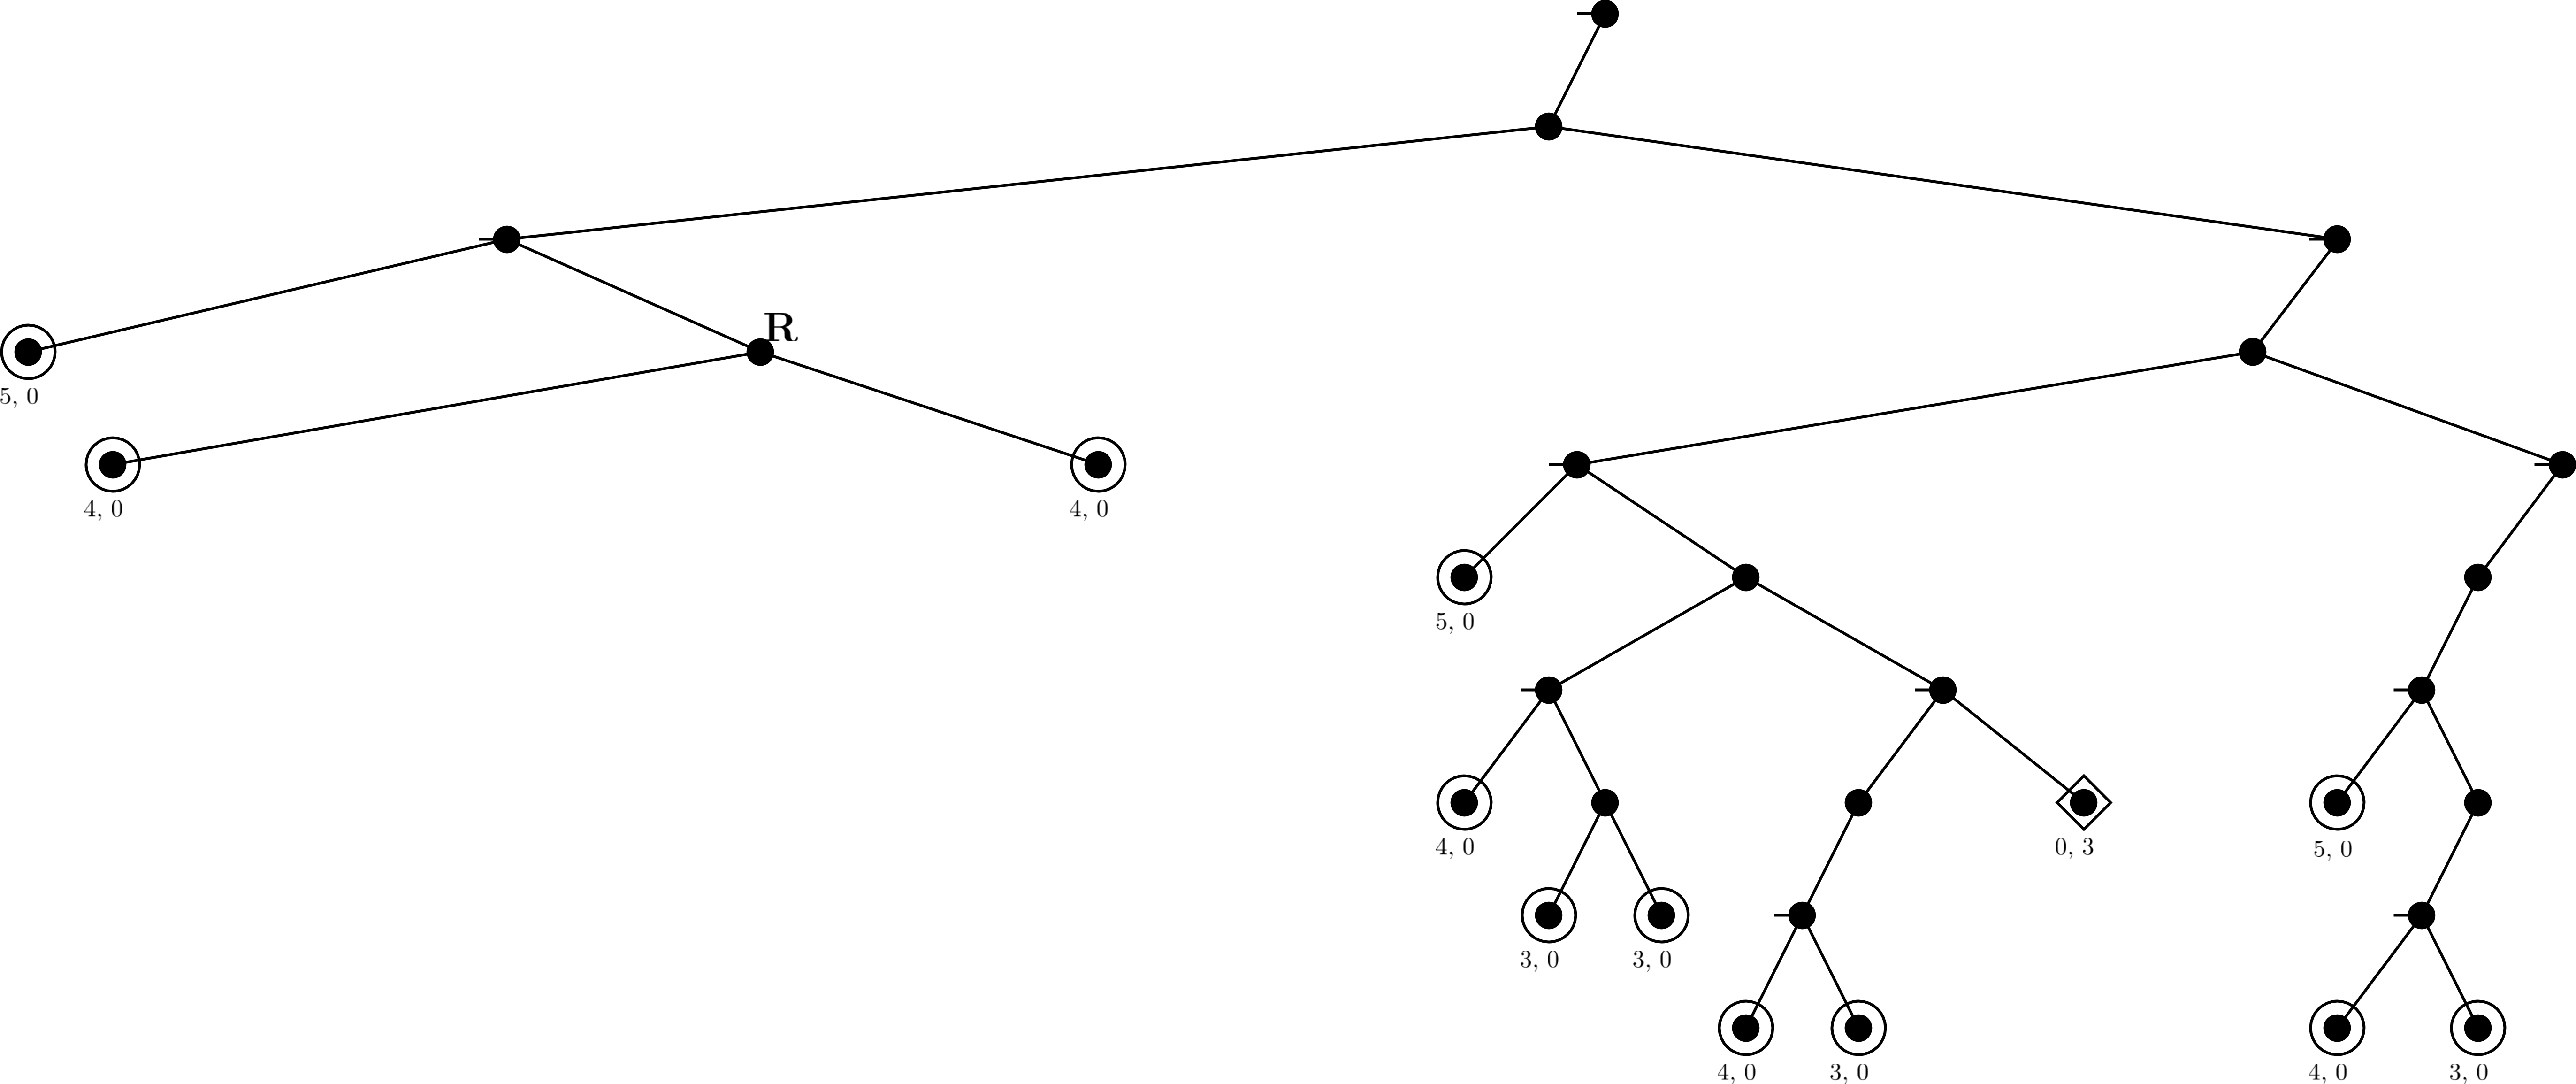
\includegraphics[width=15cm]{figures/Backwards5.png}
  \caption{The full game tree, after the backwards induction algorithm has recursed through half of the tree.}
  \label{fig:backwards5}
\end{figure}
  
Now that most of the left side of the tree has been explored by the backwards induction algorithm, we return to view the full tree in Figure \ref{fig:backwards5}. The node $R$, a decision node for Player 2, must choose between two identical leaf nodes, both with (4, 0) utility. Thus, $R$ given a utility value of (4, 0). For the final decision on the left subtree, Player 1 chooses between a (5, 0) leaf node and a (4, 0) leaf node, and will select the former. Next, the backwards induction algorithm will move to the right subtree of Figure \ref{fig:backwards5}.


\subsubsection{Analysis}
Player 1 has a huge advantage in this game by taking the first action. If both players only choose to attack, then Player 1 wins the game. The utility of this outcome is (5, 0). In fact, Player 1 can only lose by choosing to heal at certain points in the game.\\

In all four paths where player 2 won, there is a node where player 1 chose to heal from 9 HP to 10 HP. If Player 1 only attacks, then Player 2 has no chance of victory. Since the normal amount of HP recovered by healing is 4 HP, we can see that player 1 is wasting potential HP by using one of their turns to heal when their HP is already close to the HP cap. We may infer that, in games with larger HP caps, the same effects would appear. It is much more useful for a player to heal when their HP is closer to zero.\\

In this limited model, it is clear that healing is not a viable strategy. Since players can only attack or heal, one player's choice to heal will either have no effect on their utility or a negative effect on their utility. If Player 2 heals and Player 1 immediately attacks, then Player 2 has a net loss of 1 HP. The HP recovered by a player is not enough to offset the damage dealt by their opponent. If a player heals and their opponent also heals, then the difference in utility is zero. Situations where both players heal at the same time does not change the overall performance of the players. If Player 2 was losing to Player 1, and both players heal, then Player 2 will still be losing to Player 1. At the most, choosing to heal only delays the inevitable.\\

Now that some patterns in the game are identified, we expand the choices of the game and build a prototype using Python and the pygame library.

\section{Game Engine}
Python was chosen as the development language for this game. Python is an extremely portable language: anyone with Python installed can run the code. Python also has a robust library for two-dimensional games called pygame, which was essential in creating this game. Specifically, Python 3 was used for better compatibility with the pygame library and for the copy() function for arrays.

\subsection{The pygame Library}
The pygame library provides a number of Python functions that are useful in creating a two-dimensional video game. The library was originally created in 2001 to combine Python with SDL (Simple DirectMedia Layer), a library of multimedia controls written for C \cite{shinners}. pygame can utilize a variety of different graphics libraries, including OpenGL, DirectX, the Linux frame buffer, and an ASCII art backend \cite{shinners}. The pygame library is supported by numerous operating systems, and the core functions of pygame use highly optimized C or assembly code.\\

At the top level, pygame controls the initialization and exiting of its various modules, particularly the pygame.display module which renders the game. pygame features two functions to update a display window, pygame.display.flip() and pygame.display.update(). display.flip() works with two separate arrays, containing the pixel data for the window in which the game operates. One array is displayed on the screen, while the other array is used to record changes made to the on-screen image. Once all changes are made, display.flip() swaps these arrays, or ``buffers,'' by copying all the data from one array into the other. The buffer that recorded changes is now displayed on-screen, while the buffer that was displayed can now be used to record further changes. display.update() is an optimized version of flip() that takes as an argument a rectangle or a sequence of rectangles. These rectangles correspond to the areas of the display that need to be updated. For instance, passing the coordinates of a rectangle over a game's scoreboard only updates the scoreboard. With this function, large sections of the pixel array do not need to be copied from one buffer to another, speeding up the rendering process.\\

The two main objects in pygame are the Surface object and the sprite object. Surfaces can be changed with pygame to alter various attributes. For instance, the alpha value, or the transparency of the surface, can be changed with set\_alpha(). The individual color values can be converted to integers and vice versa with the map\_rgb() and unmap\_rgb() functions, respectively. This allows for pygame to store colors as a single number, rather than a tuple of integers. Surfaces are mostly used to load image files and to create backgrounds for the game. Sprites, on the other hand, are used for the actual in-game objects, such as enemies, player characters, and projectiles. Sprites can be stored in a Group object, that can be used to separate sprites by different purposes. Each sprite draws its image to a Surface, provided that it has a Surface.image and Surface.rect attribute.\\

Once a sprite or surface is created with an image, pygame can also perform graphical transformations on that image. The pygame.transform module has functions to flip, rotate, and scale an image. Another pygame feature is the ability to do collision detection on sprites and rectangles.\\

For the actual gameplay of a pygame program, there are also modules for joystick, mouse, and keyboard controls. A sound mixer module allows audio tracks to be played in the game, and the pygame.time module can be used to control the framerate of the game.

\subsection{Gameplay Design}
For the expanded version of the game, several things were changed from the game in Figure \ref{fig:gameTree}. Two additional choices were added: Parry and Strong Attack. With Parry, the player enters a guarded stance until their next turn; this player will be referred to as the defending player. If, before their next turn, their opponent attacks them, the defending player counter-attacks. The defending player loses no HP, and the player who attacked them loses 3 HP from the counter-attack. A Strong Attack does more damage than a regular attack (7 HP vs 5 HP), but has a chance to miss the opponent completely and do no damage. Additionally, a Strong Attack is unaffected by Parry; if a player is Parrying and their opponent uses a strong attack, the parry is unsuccessful and the defending player suffers 7 HP of damage.

The two players in the game begin with 25 HP each, and are able to heal twice per game. These values are stored in a PlayerAvatar class. This class also stores the type of AI used for the computer player. The class has a helper function, which is called from within the main game loop. This helper function checks which AI model is used, then calls that model's respective function.\\

Six different AI models were created. In all models, the AI checks to see if any healing turns remain; if not, the AI defaults to a normal attack. Three of the models rely on a random number generator.\\

\begin{figure}[H]
  \centering
  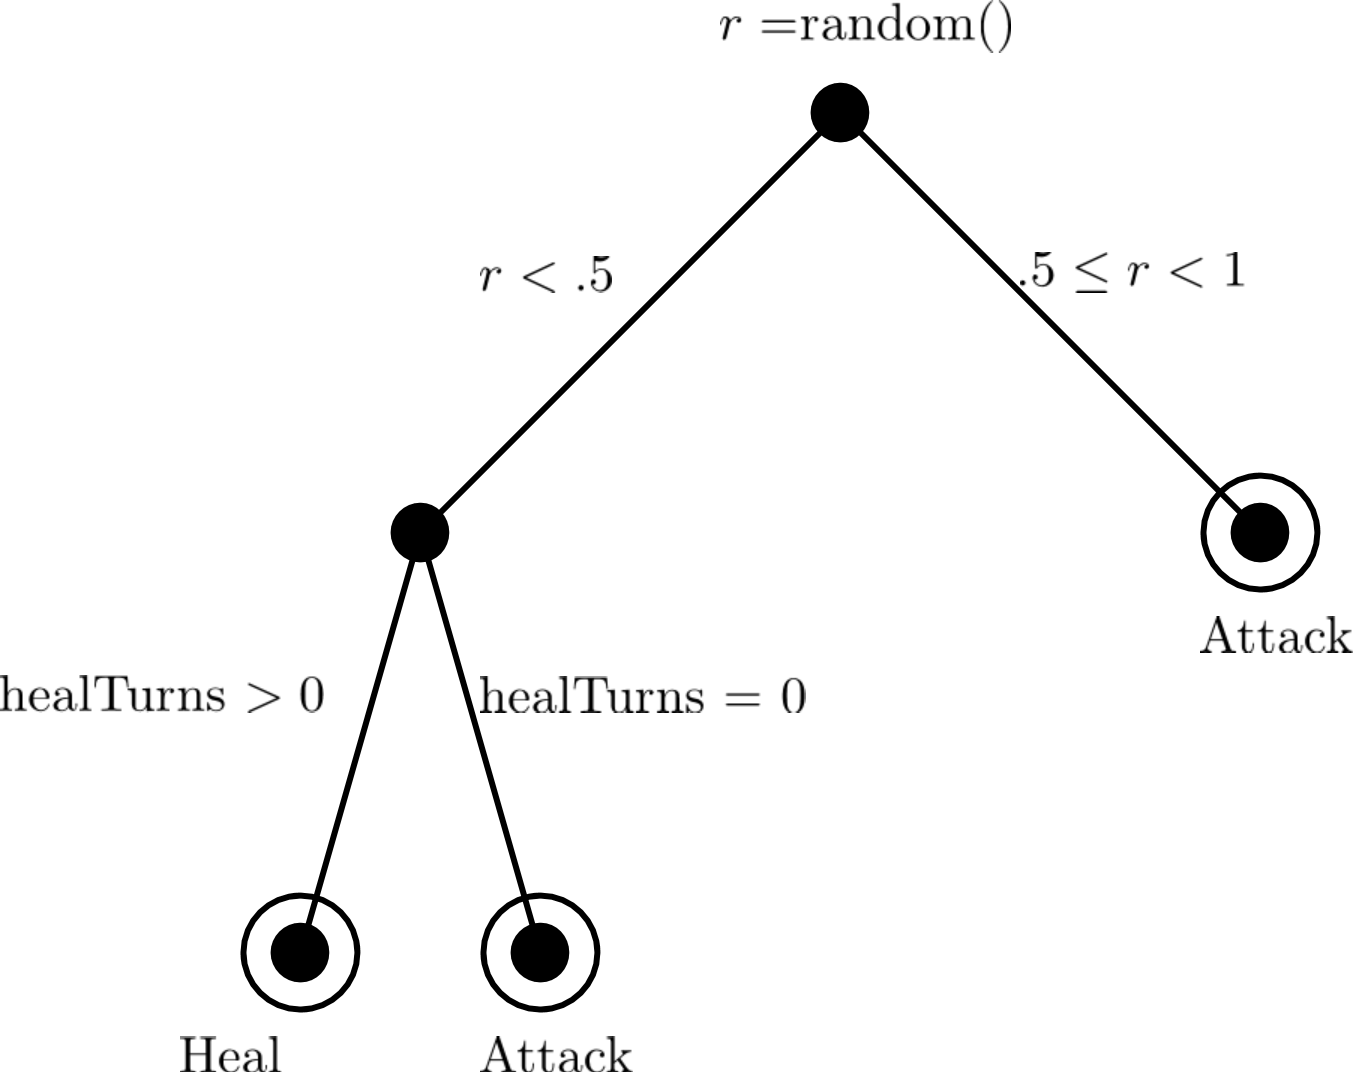
\includegraphics[width=7cm]{figures/AILimitedRandom.png}
  \caption{The decision tree for the limitedRandomAI() function.}
  \label{fig:AI1}
\end{figure}

The first AI model, the limitedRandomAI() function, chooses randomly to attack or heal with a 50/50 chance of either, but will attack instead if the AI has already healed itself twice. This is shown by the decision tree in Figure \ref{fig:AI1}. The variable $r$ is given a random value between 0 and 1, and the first decision in the tree is based on the value of $r$. After that, the tree has either reached a leaf node (for $r\ge .5$) or must make a second decision, this time based on the number of heal turns remaining. Given the limited success player 2 had in the original game tree in Figure \ref{fig:gameTree}, this model was not used in the final version of the game. Instead, a different model was used which could perform all four possible actions.\\

\begin{figure}[H]
  \centering
  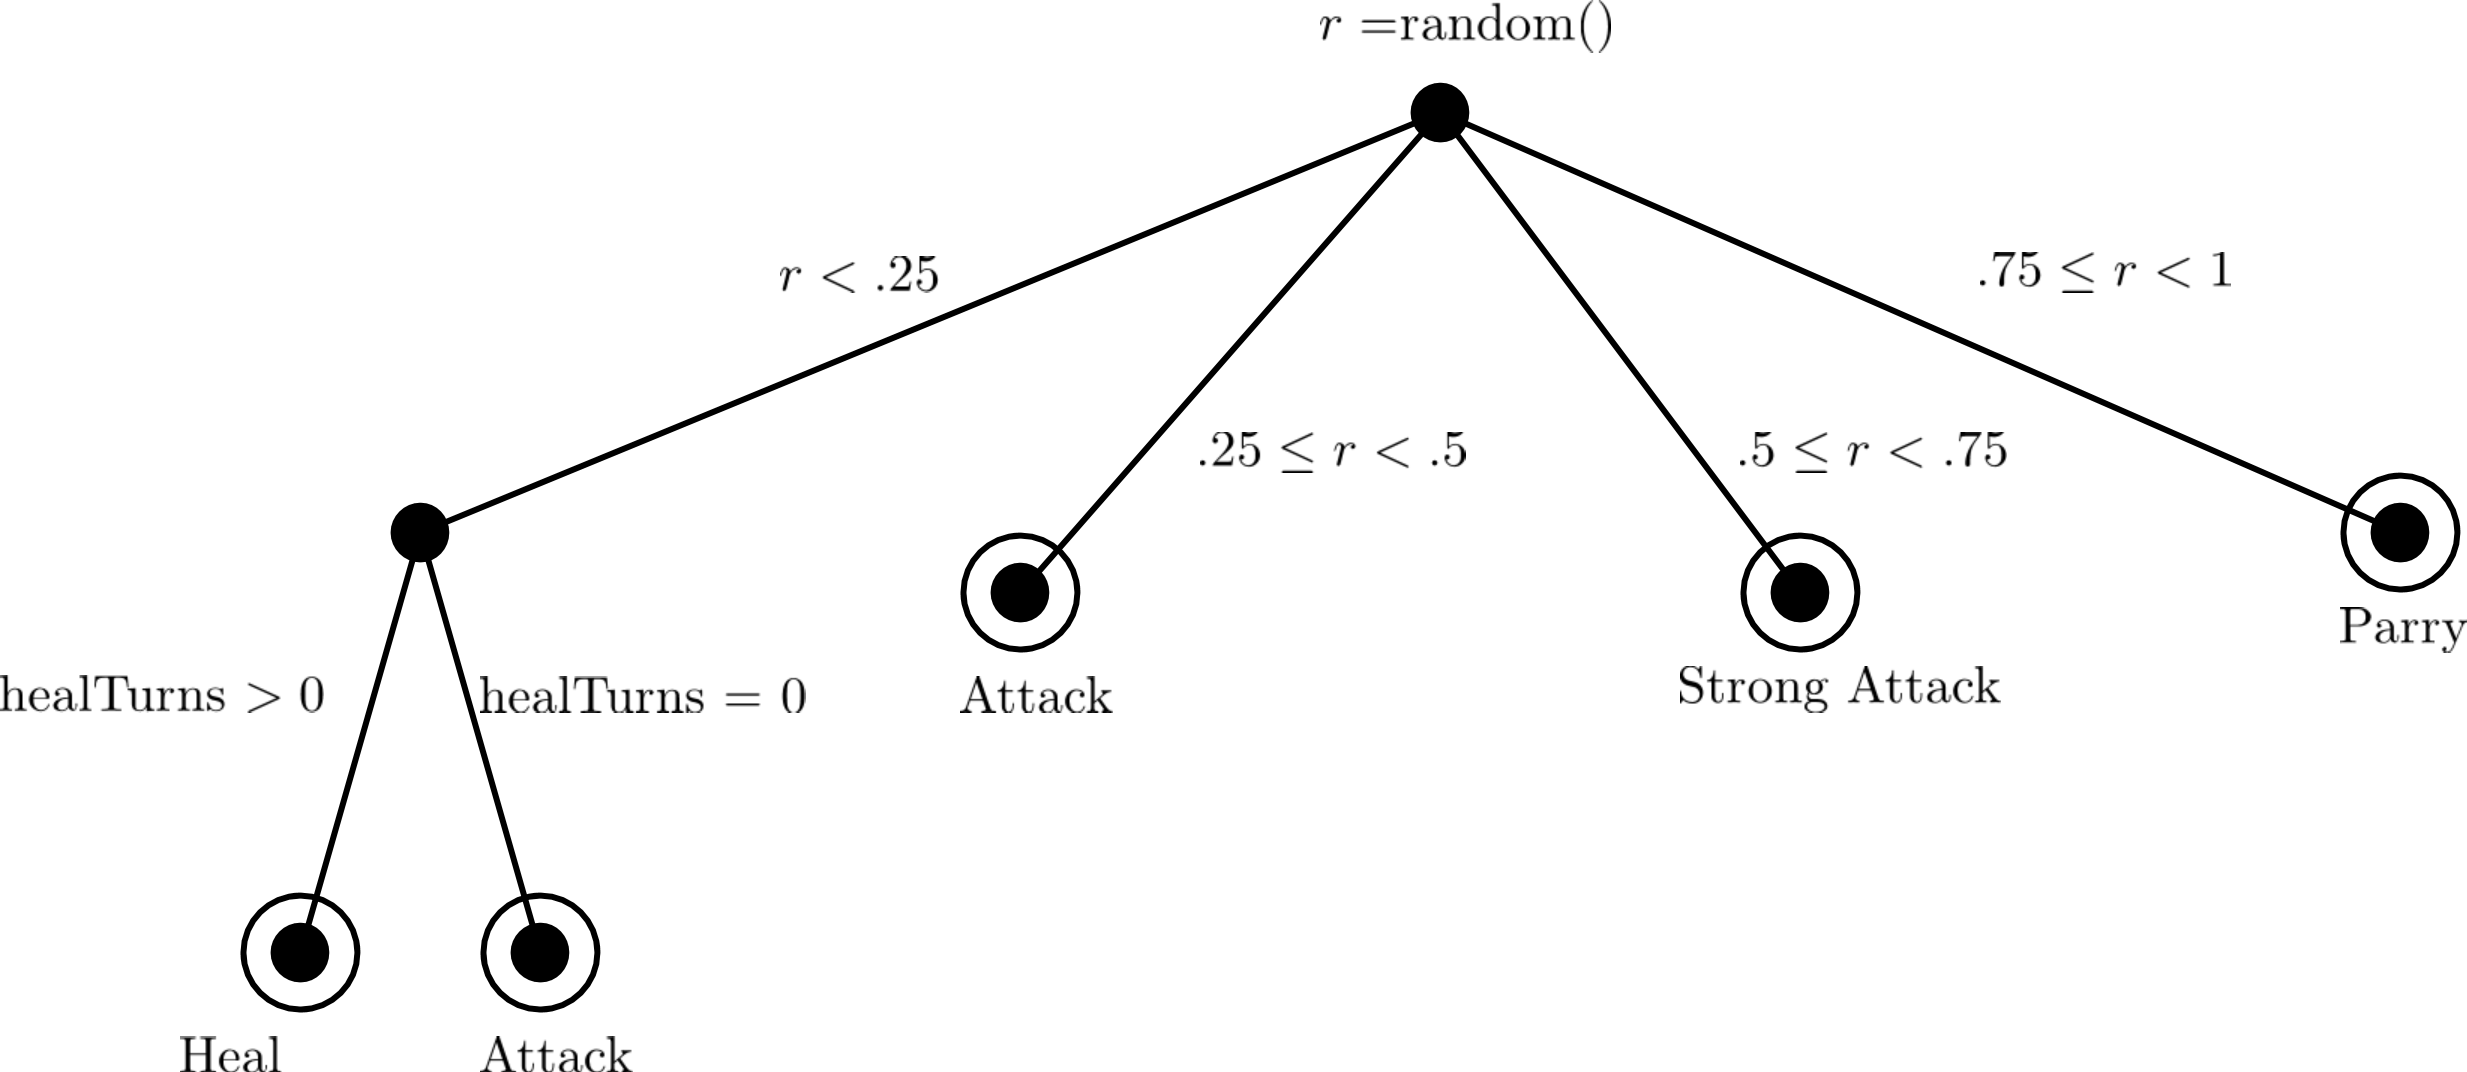
\includegraphics[width=11cm]{figures/AIRandom.png}
  \caption{The decision tree for the randomAI() function.}
  \label{fig:AI2}
\end{figure}
The second model, randomAI(), has a 25\% chance of attacking, healing, parrying, or using a strong attack. Again, Figure \ref{fig:AI2} shows that if the random number generator chooses to heal, but all healing turns have been used, the AI does a normal attack instead. This choice was made to effect a kind of desperation to fights: when an opponent no longer can heal themselves, they become more offensive to try and win the battle. This kind of behavior - where the AI changes their strategy after all healing turns have been spent - is incorporated into all the models.\\

\begin{figure}[H]
  \centering
  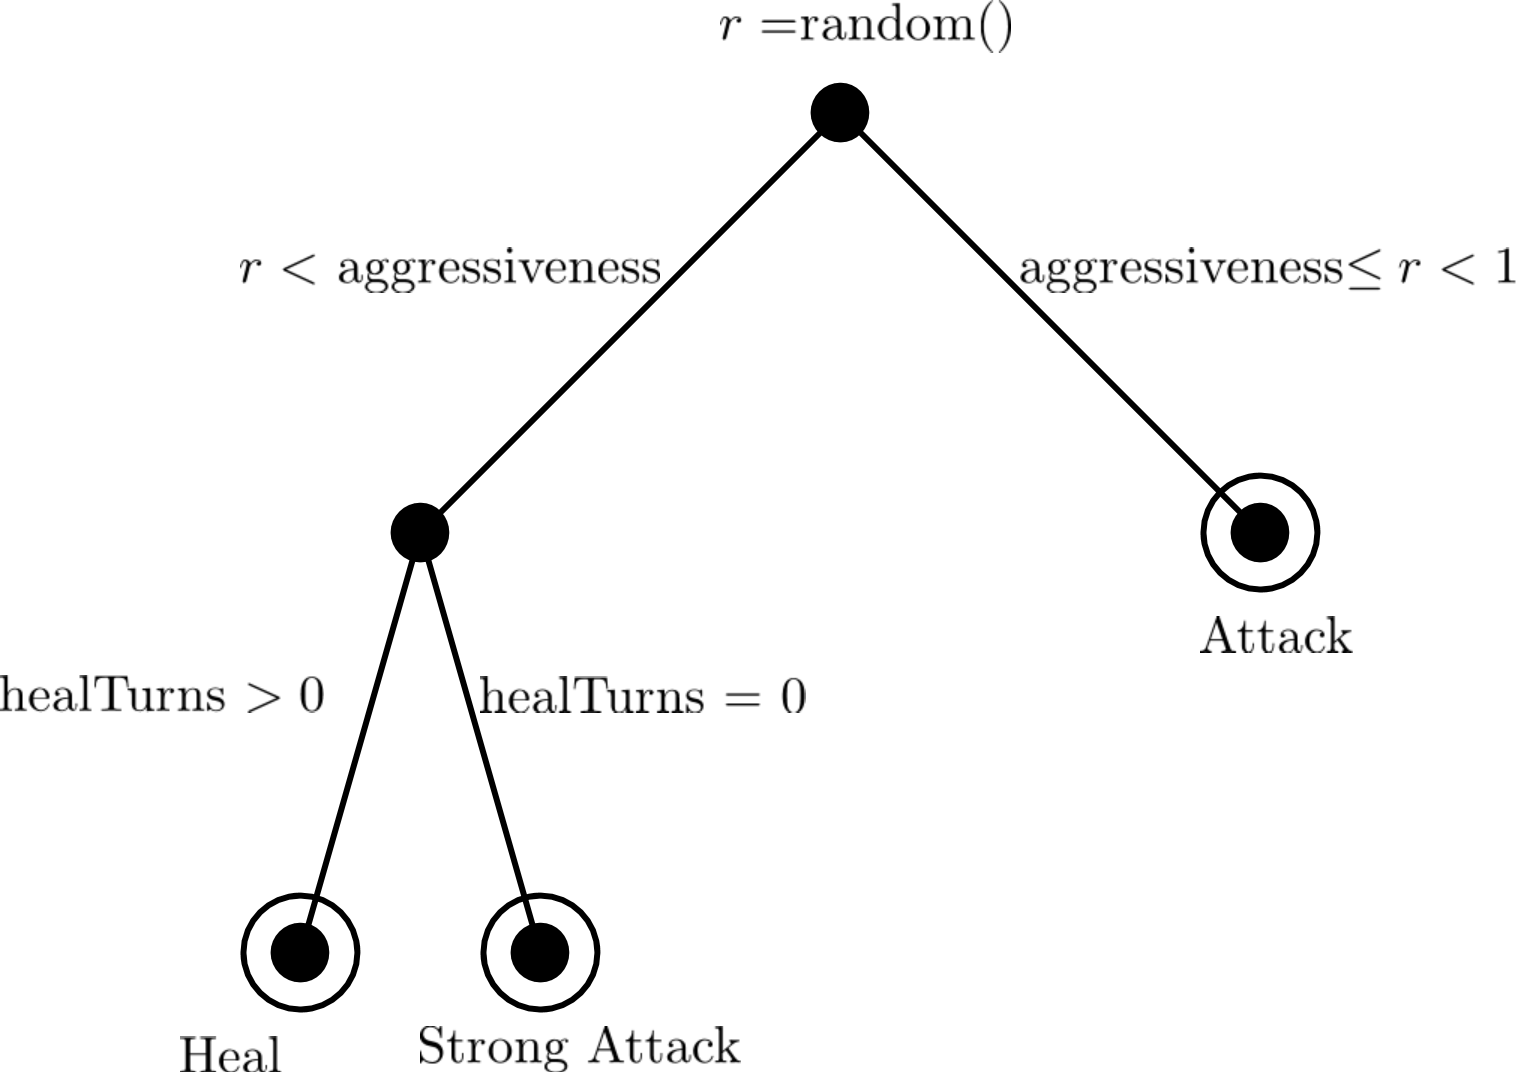
\includegraphics[width=9cm]{figures/AIAgressive.png}
  \caption{The decision tree for the aggressiveRandomAI() function.}
  \label{fig:AI3}
\end{figure}

The third model, aggressiveRandomAI(), is the final model which uses a random number generator. For this model, there is an additional variable given to the AI player, the aggressiveness stat. Rather than evenly splitting up actions 50-50, the choice between attacking and healing is split along this aggressiveness, which is a real number between 0 and 1. For this thesis, the aggressiveness was set to .25, leading to an AI which attacked 75\% of the time and healed 25\% of the time. As can be seen in the decision tree in Figure \ref{fig:AI3}, the AI uses strong attacks when the random number $r$ is below the aggressiveness stat and the two allotted heal turns are expended.

\begin{figure}[H]
  \centering
  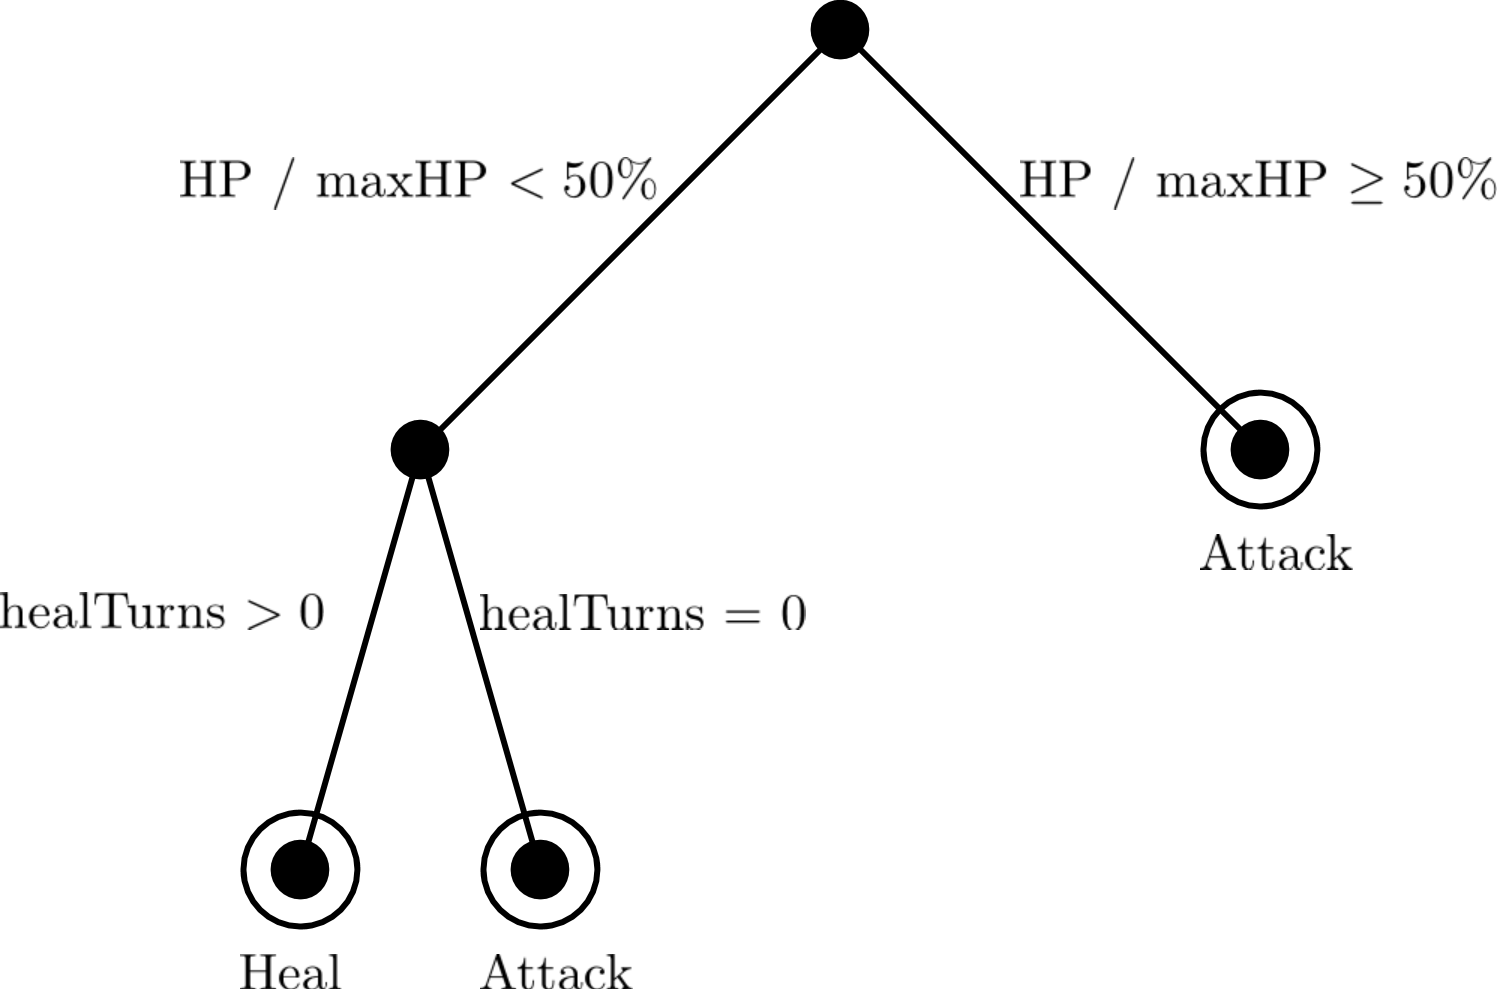
\includegraphics[width=9cm]{figures/AI50Percent.png}
  \caption{The decision tree for the fiftyPercentAI() function.}
  \label{fig:AI4}
\end{figure}

In the fourth model, fiftyPercentAI(), the AI only heals when its health falls below 50\% of its maximum. Thus, the AI only heals when it is close to death, as opposed to the random AI models which could potentially waste their heals at the start of a game. As shown in Figure \ref{fig:AI4}, this AI only uses normal attacks and heals; it does not do any parrying or strong attacks. Thus, it has the most in common with the limitedRandomAI() function with regards to possible actions. However, by saving heals until later in the game, this model has some semblance of intelligence, whereas the limitedRandomAI() does not.

\begin{figure}[H]
  \centering
  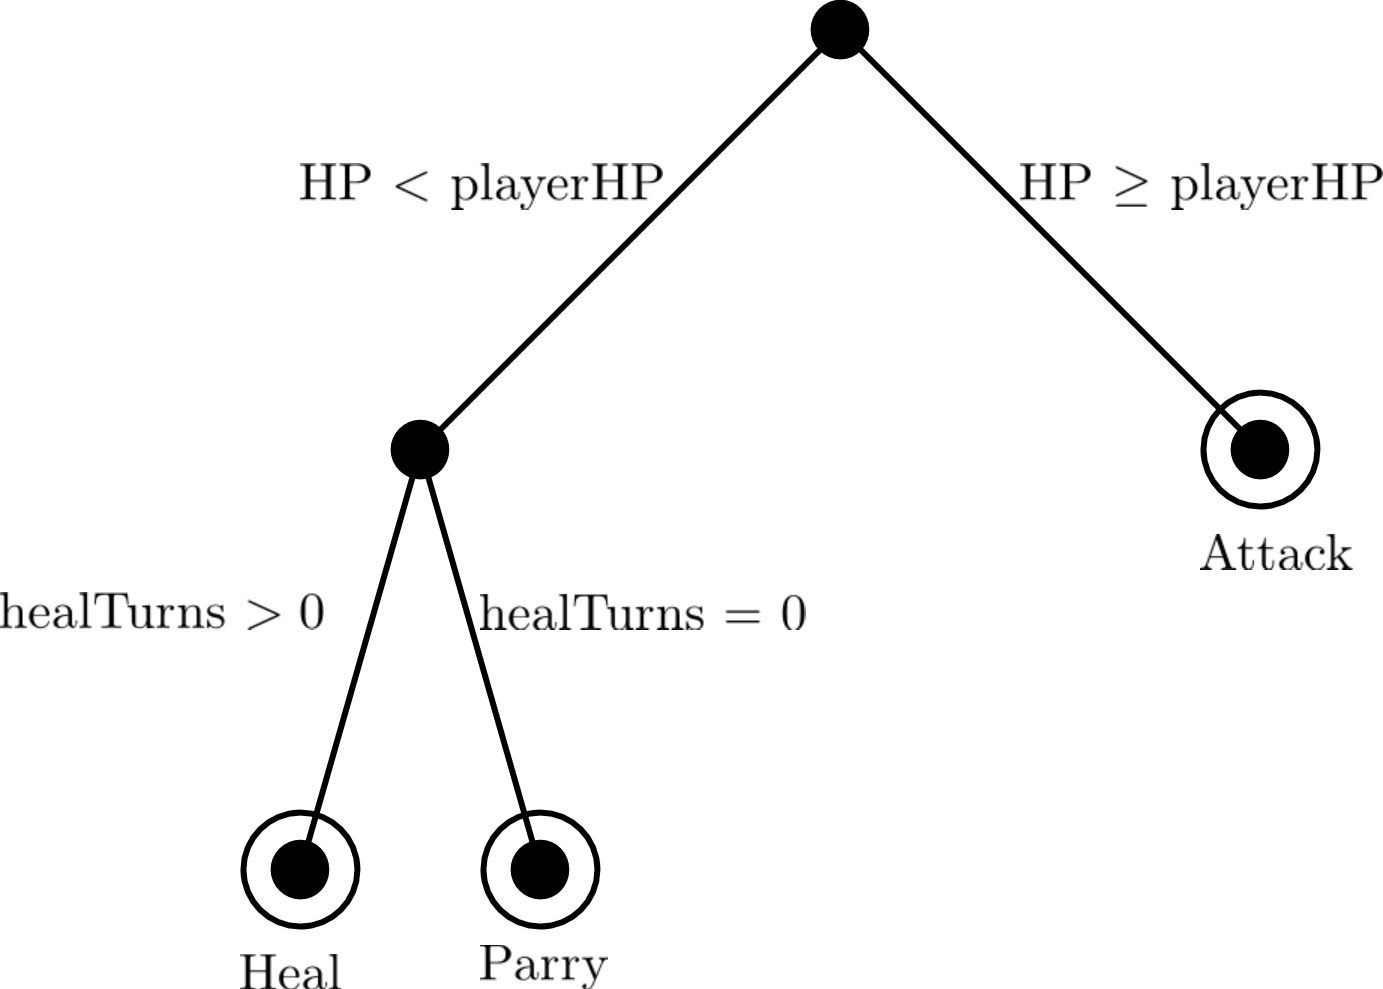
\includegraphics[width=8cm]{figures/AIComparative.png}
  \caption{The decision tree for the comparativeAI() function.}
  \label{fig:AI5}
\end{figure}

The fifth model uses similar tactics as fourth, but instead of using 50\% as the threshold, the AI heals whenever its HP drops below the player's HP, as seen in Figure \ref{fig:AI5}. Additionally, when the AI has expended all its healing turns and its HP falls below the player's HP, the AI uses a parry instead of an attack. Over the course of a game, the AI will defend itself, relying on counter-attacks to weaken the player before making attacks of its own.

\begin{figure}[H]
  \centering
  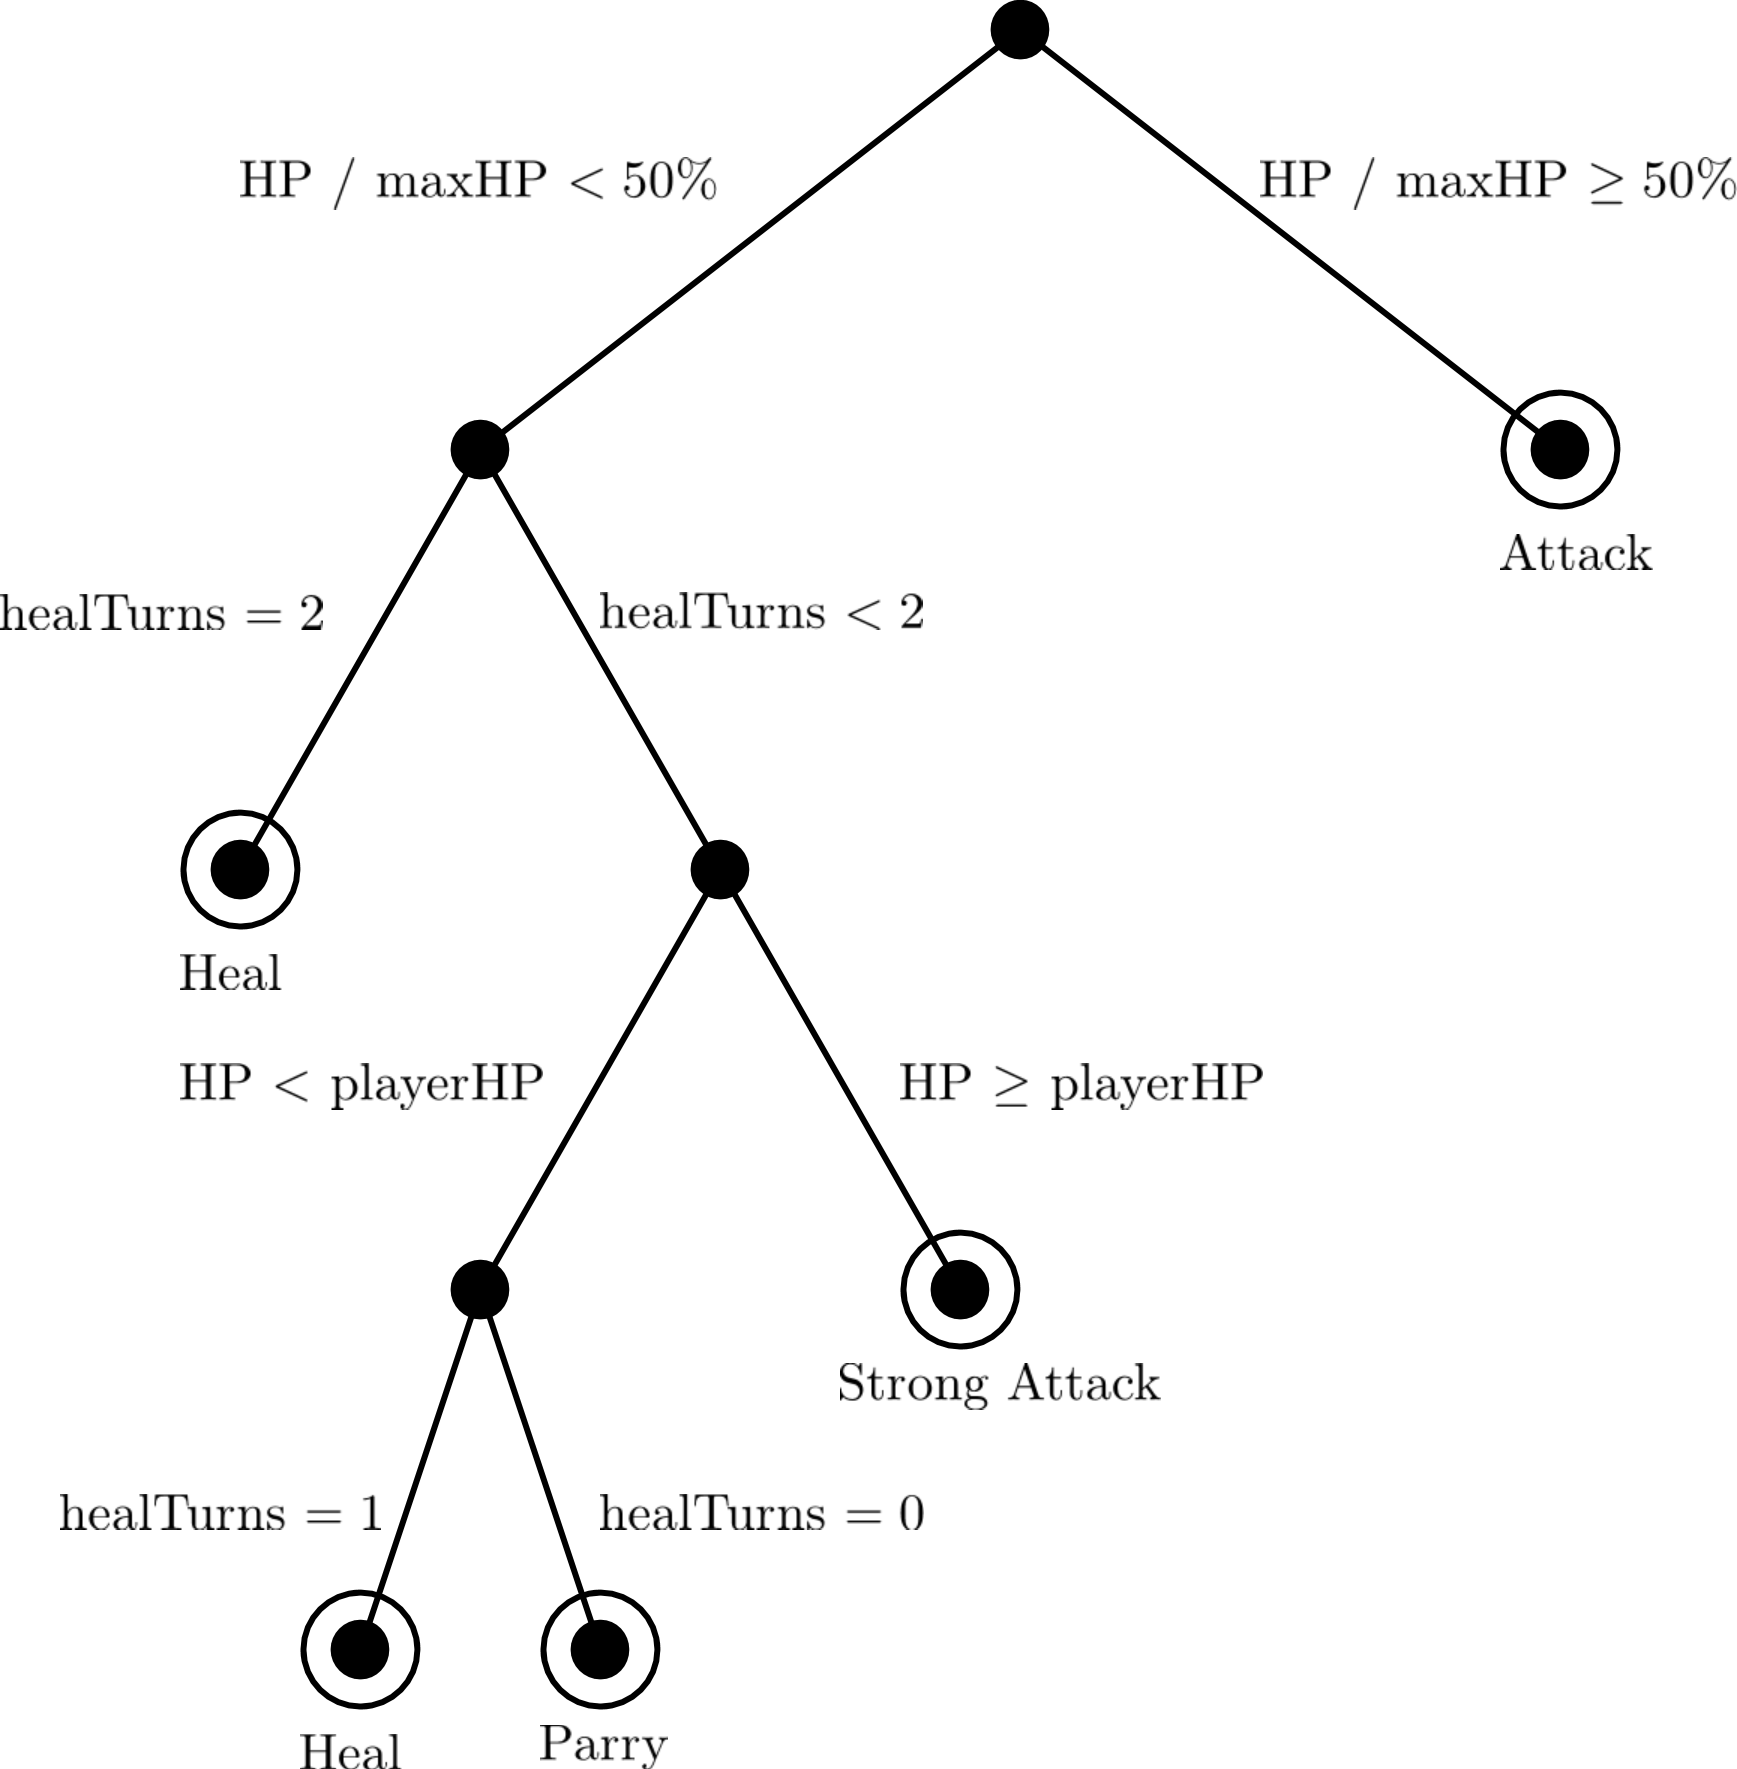
\includegraphics[width=10cm]{figures/AIScaling.png}
  \caption{The decision tree for the scalingDifficulty() function.}
  \label{fig:AI6}
\end{figure}

Finally, the scalingDifficulty() model in Figure \ref{fig:AI6} is a loose combination of the fiftyPercentAI() and comparativeAI() functions. As in \ref{fig:AI4}, the AI performs a normal attack whenever the AI's HP is above 50\% of its maximum. In this model, the two available healing turns are used in different circumstances. The first healing turn is used when the AI drops below 50\% HP for the first time. If their HP drops below 50\% after this first healing turn, the AI becomes more strategic. If the AI is below 50\% but still has a greater HP value than the player, then the AI will use strong attacks. However, if the AI is both below 50\% and below the player's HP, then it will use its second healing turn if available and parry if no healing turns remain.\\

\subsection{Visual Design}
The visual design of the game was left fairly simple, to avoid distracting players from the strategic elements of the game. Icons for the player character and enemy opponents were created in the GNU Image Manipulation Program (GIMP), then imported as pygame sprites using the pygame.image.load() function. Since these sprites had a transparency component, the function convert\_alpha() was also used to preserve this transparency in pygame.\\

\begin{figure}[H]
  \centering
  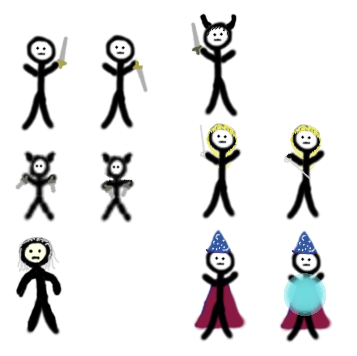
\includegraphics[width=9cm]{sprites/SpriteSheet.png}
  \caption{The set of sprites used for the characters in \textit{Cave Escape}. Clockwise from top left, the characters are the player character, an orc, an elf, a magician, a troll, and a goblin.}
  \label{fig:SpriteSheet}
\end{figure}

\begin{figure}[H]
  \centering
  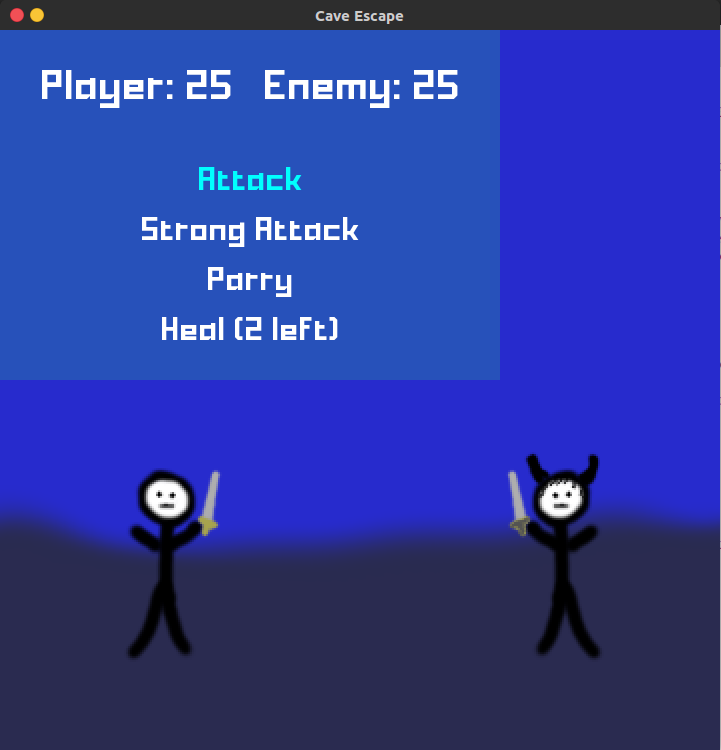
\includegraphics[width=7cm]{figures/In-Game.png}
  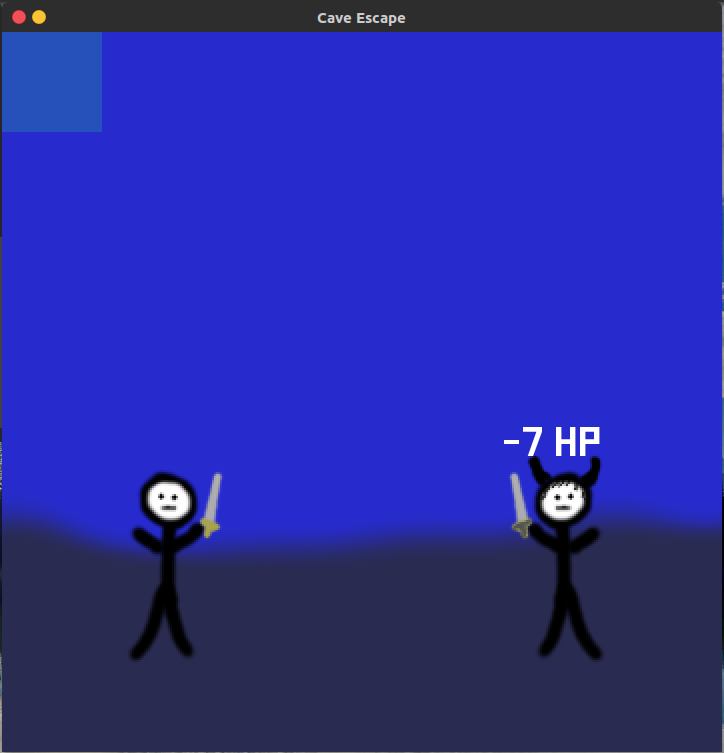
\includegraphics[width=7cm]{figures/In-Game2.png}
  \caption{In-game screenshots from \textit{Cave Escape}. The player character is situated on the left, while the opponent - an orc - is stationed on the right. The HP values of both player and AI are listed at the top of the screen. In the left image, the player is able to select their next move from the list of options. In the right image, the player has selected ``Strong Attack'' and the resulting damage is shown above the enemy's head.}
  \label{fig:ingame}
\end{figure}

An individual sprite was created for the player character and each of the five AI models, as shown in Figure \ref{fig:SpriteSheet}. These sprites are overlain on a bluish-purple background, symbolizing the cave interior. The list of possible actions is also shown on-screen, positioned above the player character as in Figure \ref{fig:ingame}. Next to the ``Heal'' option, the number of remaining healing turns is listed and updated after each turn. The HP of both players is also updated after every turn. Additionally, after players select an action, the resulting change in HP is shown above the head of the respective target. The right image in Figure \ref{fig:ingame} shows that the orc was hit by a strong attack made by the player, and took 7 points of damage.\\

Each non-player character has a respective AI model which it uses. The goblin uses the randomAI() function in Figure \ref{fig:AI2}, where all actions have a 25\% chance of being chosen. The troll uses aggressiveRandomAI(), as seen in Figure \ref{fig:AI3}. This character attacks more often that it heals, and can perform strong attacks after both healing turns are spent. The orc uses the fiftyPercentAI() function from Figure \ref{fig:AI4}. The elf is assigned to the comparativeAI() function seen in Figure \ref{fig:AI5}, and finally the magician uses the scalingDifficulty() function from Figure \ref{fig:AI6}.

\begin{figure}[H]
  \centering
  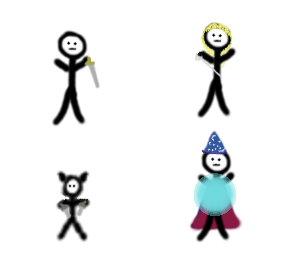
\includegraphics[width=9cm]{sprites/ParrySheet.png}
  \caption{The set of sprites used when a character is parrying. Clockwise from top left, the characters able to parry are the player character, an elf, a magician, and a goblin.}
  \label{fig:ParrySheet}
\end{figure}

In addition to the default sprites shown in Figure \ref{fig:SpriteSheet}, characters have a second sprite for when they are parrying. The Troll and Orc characters are unable to parry, so only four of these sprites were created. These variants are shown in Figure \ref{fig:ParrySheet}: the player character, the elf, the magician, and the goblin all have parry sprites.\\

At runtime, the game starts at a menu screen, where the five enemy characters are listed. When the HP of either the player or the AI falls to 0 or lower, the round ends. A final screen is shown to either celebrate the player's victory or lament their failure. The menu was made using code from a \textit{Tetris} clone made with pygame created by Dimitris Strovolidis, released under the GNU General Public License, version 3 \cite{tetris}. This code contains a ``menu'' class which allows both for interactive menus and easily-positioned text. The enemy characters are listed in this menu, and players are able to select which opponent they wish to fight.

\section{Playtesting and Survey}
To test the effectiveness of these AI models, a group of participants were surveyed to play the various models. Each participant played five rounds against one of the models. The program collects data on wins and losses, as well as the sequence of actions taken by both the human player and the AI opponent. In addition to this game data, a short survey was given to each participant. Subjects were asked to answer the first three questions before playing the game. These questions asked participants to rate, on a scale of 1 to 5, their interests in video games, strategic board games, and RPGs, respectively. A score of 1 indicated little or no interest, while a score of 5 indicated a strong interest. After the three questions, participants were given a short description of the game, including the possible actions that players could take in the game. After the participant completed the five rounds, they were asked three more questions. These questions asked them to rate, on a scale of 1 to 5, how fun they found the game, how understandable the controls were, and how aggressive or passive their playstyle. 1 indicates a rating of not fun, that the controls were not understandable at all, and that the player used a very passive playstyle, respectively. A 5 rating indicated that the participant had a lot of fun, that the controls were very understandable, and that their playstyle was very aggressive, respectively.\\

\begin{figure}[H]
  \centering
  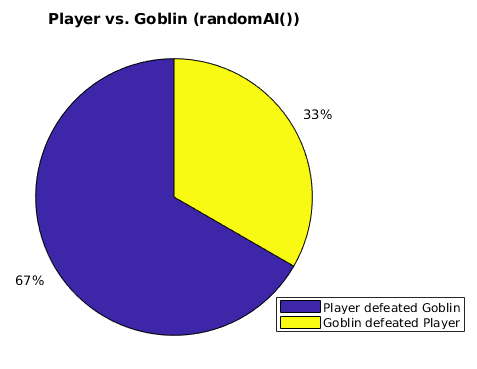
\includegraphics[width=8cm]{figures/goblinWins.png}
  \caption{The win/loss percentages for the randomAI() function, assigned to the Goblin character.}
  \label{fig:pieGoblin}
\end{figure}
After 15 individual games against the Goblin AI - using the randomAI function - the win percentage for the survey participants are as shown in \ref{fig:pieGoblin}: a 67\% win percentage for the human player, and a 33\% win percentage for the Goblin. Since this AI model uses a random number generator to determine its actions, this win percentage suggests that unpredictability is more difficult for human players to defeat. Furthermore, we can see that the expanded version of the game, with 25 HP instead of 10 and two more abilities, has more outcomes where player 2 can win.\\

\begin{figure}[H]
  \centering
  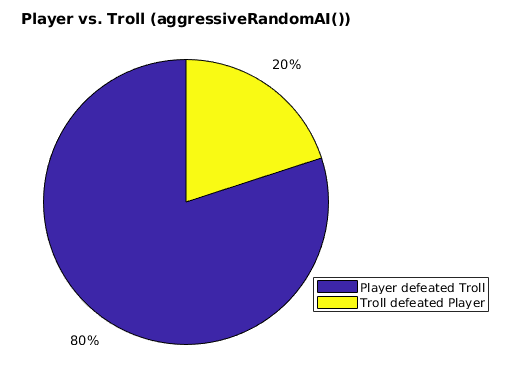
\includegraphics[width=8cm]{figures/trollWins.png}
  \caption{The win/loss percentages for the aggressiveRandomAI() function, assigned to the Troll character.}
  \label{fig:pieTroll}
\end{figure}

The Troll AI fared much worse than the Goblin, as seen in Figure \ref{fig:pieTroll}. The aggressive AI was only able to win 20\% of its games. In comparison to the Goblin, the Troll is less likely to use strong attacks; the Goblin can use a strong attack whenever, but the Troll must first expend both of their healing turns before it can use a strong attack. Additionally, the Goblin can parry while the Troll cannot. Thus, at any particular turn of the game, the Troll has a more limited move set than the Goblin.\\

\begin{figure}[H]
  \centering
  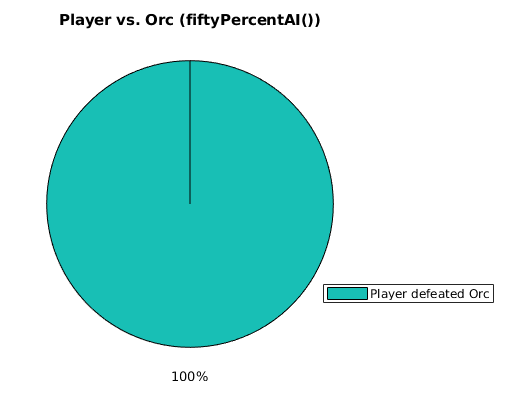
\includegraphics[width=8cm]{figures/orcWins.png}
  \caption{The win/loss percentages for the fiftyPercentAI() function, assigned to the Orc character.}
  \label{fig:pieOrc}
\end{figure}

The Orc AI performed the worst of all, as is evident from Figure \ref{fig:pieOrc}. Not a single person lost to the Orc after 15 trials. The Orc also has the most limited move set of the five models, only able to heal and use normal attacks. Seeing as the Orc has the same available moves as the players in the simple simulation in Figure \ref{fig:gameTree}, it is unsurprising that the Orc has trouble winning games.

\begin{figure}[H]
  \centering
  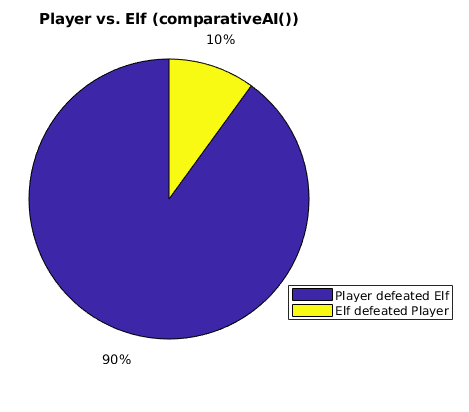
\includegraphics[width=8cm]{figures/elfWins.png}
  \caption{The win/loss percentages for the comparativeAI() function, assigned to the Elf character.}
  \label{fig:pieElf}
\end{figure}

Figure \ref{fig:pieElf} shows that the comparativeAI() function was only slightly successful. After 10 trials, the human players won 90\% of the games while the AI won 10\% of the games. Since this model uses parries frequently, a player is able to safely heal themselves without immediately losing that HP on the Elf's next attack. Furthermore, a successful parry deals 3 damage, but a successful strong attack deals 7 damage. Thus, a player can take a few hit from parries but still come out ahead with strong attacks.

\begin{figure}[H]
  \centering
  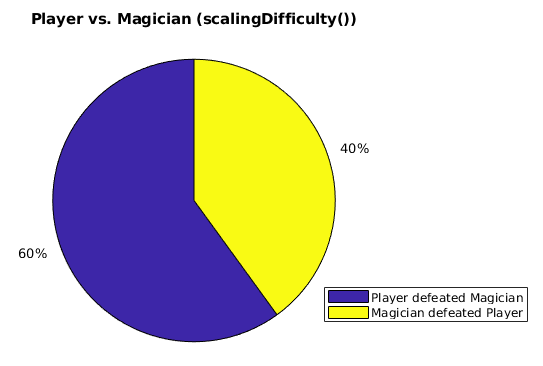
\includegraphics[width=8cm]{figures/magicianWins.png}
  \caption{The win/loss percentages for the scalingDifficulty() function, assigned to the Magician character.}
  \label{fig:pieMagician}
\end{figure}

Finally, the Magician character had the best overall record, as seen in Figure \ref{fig:pieMagician}: a win rate of 60\% for the player and 40\% for the Magician. Like the Goblin, the Magician is able to perform all four of the available actions, which the other three AI models could not do. It may be the case that, by limiting the available actions for the other AI models, they were handicapped in a way that the Goblin and Magician were not.\\


%\chapter{Future Work}

%%%%%%%%%%%%%%%%%%%%%%%%%%%%%%%%%%%%%%%%%%%%%%%%%%%%%%%
%
%  This section starts the back matter. The back matter includes appendices, indicies, and the
%  bibliography
%
%%%%%%%%%%%%%%%%%%%%%%%%%%%%%%%%%%%%%%%%%%%%%%%%%%%%%%%

\backmatter

%\input{appendices/math}
%\input{appendices/java}
%\input{appendices/cpp}
%\input{appendices/afterword}

%%%%%%%%%%%%%%%%%%%%%%%%%%%%%%%%%%%%%%%%%%%%%%%%%%%%%%%
%
%  This section would be used if you are not using BibTeX. Look at Kopka and Daly for how to
%  format a bibliography manually as well as how to use BibTeX.
%
%%%%%%%%%%%%%%%%%%%%%%%%%%%%%%%%%%%%%%%%%%%%%%%%%%%%%%%

%\begin{thebibliography}{99}
%\bibitem{}
%\bibitem{}
%\end{thebibliography}

%%%%%%%%%%%%%%%%%%%%%%%%%%%%%%%%%%%%%%%%%%%%%%%%%%%%%%%
%
%  We used BibTeX to generate a Bibliography. I would recommend this method. However, it is
%  not required.
%
%%%%%%%%%%%%%%%%%%%%%%%%%%%%%%%%%%%%%%%%%%%%%%%%%%%%%%%

\renewcommand\bibname{References} % changes the name of the Bibliography

\nocite{*}% This command forces all the bibliography references to be printed -- not just 
           % those that were explicitly cited in the text.  If you comment this out, the
           % bibliography will only include cited references.
%\ifthenelse{\boolean{woosterchicago}}{
%  \bibliographystyle{woosterchicago}}
%{\ifthenelse{\boolean{achemso}}{
%    \bibliographystyle{achemso}}
\bibliographystyle{plainnat}
% if you have used the woosterchicago class option then your references and citations will be in Chicago format. If you have used the achemso class option then your references and citations will be in the American Chemical Society format. If you do not specify a citation format then the default Wooster format will be used.
\bibliography{references} % load our Bibliography file

%%%%%%%%%%%%%%%%%%%%%%%%%%%%%%%%%%%%%%%%%%%%%%%%%%%%%%%
%
%                                                                Index
%
%  Uncomment the lines below to include an index. To get an index you must put 
%  \index{index text} after any words that you want to appear in the index.
%  Subentries are entered as \index{index text!subentry text}. You must also run the
%  makeindex program to generate the index files that LaTeX uses. The PCs are set to run
%  makeindex automatically.
%
%%%%%%%%%%%%%%%%%%%%%%%%%%%%%%%%%%%%%%%%%%%%%%%%%%%%%%%

\ifthenelse{\boolean{index}}{
\cleardoublepage
\phantomsection
\addcontentsline{toc}{chapter}{Index}
\printindex}{}

%%%%%%%%%%%%%%%%%%%%%%%%%%%%%%%%%%%%%%%%%%%%%%%%%%%%%%%
%
%                                                                Colophon
%
%  A Colophon is a section of a printed document that acknowledges the designers and printers of the work.
% The colophon also includes information about the fonts and paper used in the printing. It is not required 
% for your IS and can be commented out.
%
%%%%%%%%%%%%%%%%%%%%%%%%%%%%%%%%%%%%%%%%%%%%%%%%%%%%%%%

\ifthenelse{\boolean{colophon}}{
\begin{colophon}
This Independent Study was designed by Dr. Jon Breitenbucher.\newline
It was edited and set into type in Wooster, Ohio,\newline
using the \ifthenelse{\boolean{xetex}}{\XeTeX\ typesetting system designed by Jonathan Kew}{\LaTeX\ typesetting system designed by Leslie Lamport}\newline
and based on the original \TeX\ system of Donald Knuth.\newline
It was printed and bound by Office Services at The College of Wooster.

The text face is Adobe Garamond Pro, designed by Robert Slimbach.\newline
This is the Opentype version distributed by Adobe Systems\newline
and purchased as part of the Adobe Type Classics for Learning.

The paper is standard laser copier paper and not of archival quality.
\end{colophon}}{}
\clearpage\thispagestyle{empty}\null\clearpage
\end{document}